\chapter{A Formal Proof of Correctness Requirements
    \pgsize{25 p.}
}

\todo{Restructure into formalization of correctness (containing compatibility, interoperability etc.) and formal proof of proving correctness. Or maybe move that to prevention section?}

Allgemeine Definition Transformationsnetzwerke:
\begin{itemize}
    \item Definition Transformation aus Relation und Wiederherstellungsroutinen; Routinen nehmen n Modelle und n Deltasequenzen (eine pro Modell) und liefern n Deltasequenzen zurück.
    \item Im Allgemeinen könnte eine Transformation beliebige dieser Deltasequenzen modifizieren. Wir verlangen jedoch, dass eine Transformation nur Deltas anhängt, also die Sequenzen länger werden
    \item Genauer beschränken wir auch, welche Sequenzen eine Transformation sehen und ändern darf, genau gesagt darf sie die Sequenzen von zwei Modellen sehen und eine davon verlängern.
    \item Hier kommt bereits der Unterschied zu bisherigen Transformationen, denn die sehen nur Deltas an einem Modell und erzeugen Deltas an dem anderen. Das ist bei uns schon gänzlich anders. Bidirektionale Transformationen unterstützen das im Übrigen auch nicht, sondern sind nur Spezifikationen, aus denen sich Wiederherstellungsroutinen für beide Richtungen ableiten lassen (siehe Stevens 2010)
    \item Relationen in erster Instanz auf Modellebene (also bzgl. ganzer Modelle, nicht einzelner Modellelemente) definieren
    \item Direkt als multidirektionale Transformation definieren, also beliebig viele geändert Ein- und Ausgabemodelle (oder jeweils nur eins?)
    \item Korrektheit einer Transformation (nach Stevens) definieren!
    \item Versuchen den Konkatenationsoperator zu definieren ohne dass er alle Metamodelle referenzieren muss (also Transformation wählt aus einer großen Eingabemenge relevanten Modelle aus, ändert relevante und dann fügt der Operator sie in die große Menge ein)
    \item Definition Transformationsnetzwerk als Tupel aus Metamodellen, Transformationen und einer Ausführungsfunktion. 
    \item Die Ausführungsfunktion führt für eine gegebene Änderung eine Auswahl der Transformationen nacheinander aus.
    \item Korrektheit eines Netzwerkes definieren: Die Ausführungsfunktion erzeugt eine Transformationssequenz, die angewendet auf eine Änderung für alle Änderungen ein korrektes Ergebnisse produziert, d.h. die Modelle sind konsistent bzgl. allen Konsistenzrelationen.
\end{itemize}

An intuitive way of describing consistency for an arbitrary number of metamodels is to specify all tuples of models that are considered consistent to each other, i.e., to specify a relation between the models. 

\begin{definition}[\ModelLevelConsistencyRelation]
    Given a tuple of metamodels $\metamodeltuple{M} = \tupled{\metamodelsequence{M}{n}}$, a \emph{\modellevelconsistencyrelation} $\consistencyrelation{CR}{}$ is a relation for instances of the metamodels $\consistencyrelation{CR}{} \subseteq \metamodeltupleinstanceset{M} = \metamodelinstanceset{M}{1} \times \dots \times \metamodelinstanceset{M}{n}$.
    We consider a tuple of models $\tupled{\model{m}{1}, \dots, \model{m}{n}} \in \metamodeltupleinstanceset{M}$ \emph{consistent to $\consistencyrelation{CR}{}$} if and only if $\tupled{\model{m}{1}, \dots, \model{m}{n}} \in \consistencyrelation{CR}{}$.
    Otherwise, we call $\tupled{\model{m}{1}, \dots, \model{m}{n}}$ \emph{inconsistent to $\consistencyrelation{CR}{}$}.
\end{definition}

Given a tuple of models, we consider that tuple of models consistent if it is contained in the consistency relation.
We explicitly denote this kind of consistency relation as \emph{model-level}, because we will later need a more fine-grained notion of consistency relations at the level of \metaclasses and need to distinguish between the two.

\todo{Das folgende drückt eine Definition entsprechend der Annahme der modularen Spezifikation aus. Wir stellen es später in Bezug zu globalen Konsistenzrelationen und anderen Spezifikationsmöglichkeiten, Stichwort MX}

\section{A Monolithic Notion of Consistency}

Having one consistency relation for an arbitrary number of metamodels constitutes a \emph{monolithic} notion of consistency, as it describes consistency for an arbitrary number of metamodels as a whole.
Accordingly, a multidirectional transformation~\cite{cleve2019dagstuhl} could be defined that takes a consistent tuple of models and any change to them and then returns a consistent tuple of models again, which then reflects the performed change.

\todo{Define correctness based on a networks adhering to the behavior of a multidirectional transformation}



\section{A Modular Notion of Consistency}



In the following, we only consider binary consistency relations. Having several consistency relations to define how several metamodels are related, we need to define a notion of consistency based on several consistency relationsl

\begin{definition}[Consistency]
    Let $\metamodeltuple{M} =  \tupled{\metamodelsequence{M}{n}}$ be metamodels and let $\consistencyrelation{CR}{} \subseteq \metamodelinstanceset{M}{i} \times \metamodelinstanceset{M}{j}$ be a binary \modellevelconsistencyrelation for any two metamodels $\metamodel{M}{i}, \metamodel{M}{j} \in \setted{\metamodelsequence{M}{n}}$.
    For a given tuple of models $\modeltuple{m} \in \metamodeltupleinstanceset{M}{} = \metamodelinstanceset{M}{1} \times \dots \times \metamodelinstanceset{M}{n}$, we say that this model set is \emph{consistent to} $\consistencyrelation{CR}{}$ if and only if the instances of $\metamodel{M}{i}$ and $\metamodel{M}{j}$ are in that relation:
    \begin{align*} 
        &
        \modeltuple{m} \consistenttomath \consistencyrelation{CR}{} \equivalentperdefinition \\
        & \formulaskip
        \exists \model{m}{i} \in \metamodelinstanceset{M}{i}, \model{m}{j} \in \metamodelinstanceset{M}{j} : \model{m}{i} \in \modelset{m} \land \model{m}{j} \in \modelset{m} \land \tupled{\model{m}{i}, \model{m}{j}} \in \consistencyrelation{CR}{}
    \end{align*}
    For a set of binary \modellevelconsistencyrelations $\consistencyrelationset{CR}$ for metamodels $\metamodelsequence{M}{n}$, we say that a given tuple of models $\modeltuple{m} \in \metamodeltupleinstanceset{M}{}$ is \emph{consistent to} $\consistencyrelationset{CR}$ if and only if the it is consistent to each consistency relation in that set:
    \begin{align*} 
        &
        \modeltuple{m} \consistenttomath \consistencyrelationset{CR} \equivalentperdefinition \\
        & \formulaskip
        \forall \consistencyrelation{CR}{} \in \consistencyrelationset{CR} : \modeltuple{m} \consistenttomath \consistencyrelationset{CR}
    \end{align*}
\end{definition}


\begin{definition}[Change]
    Given a metamodel $\metamodel{M}{}$, a change $\change{\metamodel{M}{}}$ is a function that takes an instance of that metamodel and returns another instances:
    \begin{align*}
        &
        \change{\metamodel{M}{}}: \metamodelinstanceset{M}{} \rightarrow \metamodelinstanceset{M}{}
    \end{align*}
    It encodes any kind of change, which may be just an element addition, or removal, an attribute change and so on, or any composition of changes.
    We denote the identity change, i.e., the change that always returns the input model, as $\identitychange$:
    \begin{align*}
        &
        \identitychange(x) = x
    \end{align*}
    For us, it does not matter how the function behaves in cases, in which the encoded change cannot be applied, e.g., because the changed or removed element does not exist. The function may do nothing for those models, i.e. return the identical model, or even be undefined for those model, i.e., be partial.
    \todoLater{Check whether this behavior is correct.}
    We denote the universe of all changes in $\metamodel{M}{}$, i.e. all subsets of $\metamodelinstanceset{M}{} \times \metamodelinstanceset{M}{}$ that are functional, as 
    \begin{align*}
        &
        \changeuniverse{\metamodel{M}{}} = \setted{\change{\metamodel{M}{}} \mid \change{\metamodel{M}{}} \subseteq \metamodelinstanceset{M}{} \times \metamodelinstanceset{M}{} \land
        (\tupled{\model{m}{1}, \model{m}{2}}, \tupled{\model{m}{1}, \model{m}{3}} \in \change{\metamodel{M}{}} \Rightarrow \model{m}{2} = \model{m}{3})}
    \end{align*}
    For a given metamodel tuple $\metamodeltuple{M} = \tupled{\metamodelsequence{M}{n}}$, we denote the set of all tuples of changes in the instances tuples of 
    $\metamodeltuple{M}$, i.e., 
    in $\metamodeltupleinstanceset{M}$, as $\changeuniverse{\metamodeltuple{M}}$:
    \begin{align*}
        &
        \changeuniverse{\metamodeltuple{M}} = \setted{ \changetuple{\metamodeltuple{M}} = \tupled{\change{\metamodel{M}{1}}, \dots, \change{\metamodel{M}{n}}} \mid \forall i \in \setted{1,\dots,n} : \change{\metamodel{M}{i}} \in \changeuniverse{\metamodel{M}{i}} } 
    \end{align*}
\end{definition}

\begin{definition}[\ModelLevelConsistencyPreservationRule]
    Given two metamodels $\metamodel{M}{1}, \metamodel{M}{2}$ and a binary \modellevelconsistencyrelation between them $\consistencyrelation{CR}{} \subseteq \metamodelinstanceset{M}{1} \times \metamodelinstanceset{M}{2}$.
    A \emph{\modellevelconsistencypreservationrule} $\consistencypreservationrule{\consistencyrelation{CR}{}} : (\metamodelinstanceset{M}{1}, \metamodelinstanceset{M}{2}, \change{\metamodel{M}{1}}) \rightarrow \change{\metamodel{M}{2}}$ for that consistency relation is a function that takes two consistent models and a change in the first one and returns a change in the second one, such that the resulting models when applying both changes are consistent again:
    \begin{align*}
        &
        \forall \model{m}{1} \in \metamodelinstanceset{M}{1}, \model{m}{2} \in \metamodelinstanceset{M}{2} :
        \tupled{\model{m}{1}, \model{m}{2}} \in \consistencyrelation{CR}{} \Rightarrow\\
        & \formulaskip
        \forall \change{\metamodel{M}{1}} \in \changeuniverse{\metamodel{M}{1}} :
        \exists \change{\metamodel{M}{2}} \in \changeuniverse{\metamodel{M}{2}} :\\
        & \formulaskip
        \consistencypreservationrule{\consistencyrelation{CR}{}}(\model{m}{1}, \model{m}{2}, \change{\metamodel{M}{1}}) = \change{\metamodel{M}{2}} 
        \land \tupled{\change{\metamodel{M}{1}}(\model{m}{1}), \change{\metamodel{M}{2}}(\model{m}{2})} \in \consistencyrelation{CR}{}
    \end{align*}
\end{definition}

This is equivalent to the definition of \emph{consistency restorers} in \cite{stevens2010sosym}, except that their definition is state based, thus only considering two inconsistent models states and deriving a new state of one of the models, whereas our definition is delta based, considering the changes between two models, which gives us the possibility to also take into account how the inconsistency was created and later the possibility to consider the composition of changes.

A \modellevelconsistencypreservationrule is defined to restore consistency after a modification in a left model of the underlying \modellevelconsistencyrelation by creating a change for the right model. To consider consistency preservation rules that preserve consistency in the other direction, we regard the inverse of the consistency relation as well, denoted as $\inverseconsistencyrelation{CR}{} = \setted{\tupled{\model{m}{1}, \model{m}{2}} \mid \tupled{\model{m}{2}, \model{m}{1}} \in \consistencyrelation{CR}{}}$.

A \modellevelconsistencyrelation together with two consistency restorers, or \modellevelconsistencypreservationrules in our terminology, forms a \emph{bidirectional transformation}.

\begin{definition}[Bidirectional Transformation]
    Let $\consistencyrelation{CR}{}$ be a \modellevelconsistencyrelation, and $\consistencypreservationrule{\consistencyrelation{CR}{}}$ and $\consistencypreservationrule{\inverseconsistencyrelation{CR}{}}$ two \modellevelconsistencypreservationrules to restore consistency according to that relation in both directions, i.e., after changes in any of the models.
    A bidirectional transformation is a triple $\tupled{\consistencyrelation{CR}{}, \consistencypreservationrule{\consistencyrelation{CR}{}}, \consistencypreservationrule{\inverseconsistencyrelation{CR}{}}}$.
\end{definition}

The definition could also be given for an arbitrary number of metamodels, but we restrict ourselves to binary specifications, as explained in \todoLater{ref}.

\begin{definition}[\ModelLevelConsistencyPreservationRule Generalization Function]
    Let $\consistencypreservationrule{\consistencyrelation{CR}{}}$ be a \modellevelconsistencypreservationrule for metamodels $\metamodel{M}{i}, \metamodel{M}{k}$.
    Let $\metamodeltuple{M} = \tupled{\metamodel{M}{1}, \dots, \metamodel{M}{i}, \dots, \metamodel{M}{k}, \dots, \metamodel{M}{n}}$ be a tuple of metamodels containing $\metamodel{M}{i}$ and $\metamodel{M}{j}$.
    A \modellevelconsistencypreservationrule generalization function $\cprgeneralizationfunction{\consistencypreservationrule{\consistencyrelation{CR}{}}}$ is a function:
    \begin{align*}
        &
        \cprgeneralizationfunction{\consistencypreservationrule{\consistencyrelation{CR}{}}} : (\metamodeltupleinstanceset{M}, \changeuniverse{\metamodeltuple{M}} \Rightarrow (\metamodeltupleinstanceset{M}, \changetuple{\metamodeltuple{M}})
    \end{align*}
    It generalizes $\consistencypreservationrule{\consistencyrelation{CR}{}}$ such that it can be applied to changes in $\metamodeltuple{M}$ instead of $\metamodel{M}{i}$, i.e. it applies the change delivered by $\consistencypreservationrule{\consistencyrelation{CR}{}}$ for the relevant models to the given change tuple:
    \begin{align*}
        &
        \forall \modeltuple{m} = \tupled{\model{m}{1}, \dots, \model{m}{i}, \dots, \model{m}{k}, \dots, \model{m}{n}} \in \metamodeltupleinstanceset{M}:\\
        &
        \forall \changetuple{\metamodeltuple{M}} = \tupled{\change{\metamodel{M}{1}}, \dots, \change{\metamodel{M}{i}}, \dots, \change{\metamodel{M}{k}}, \dots, \change{\metamodel{M}{n}}} \in \changeuniverse{\metamodeltuple{M}} : \\
        & \formulaskip
        \exists \change{\metamodel{M}{k}}' \in \changeuniverse{\metamodel{M}{k}} : \change{\metamodel{M}{j}}' = \consistencypreservationrule{\consistencyrelation{CR}{}}(\model{m}{i}, \model{m}{k}, \change{\metamodel{M}{i}})\\
        & \formulaskip
        \land \cprgeneralizationfunction{\consistencypreservationrule{\consistencyrelation{CR}{}}}(\modeltuple{m}, \changetuple{\metamodeltuple{M}}) = (\modeltuple{m}, \tupled{\change{\metamodel{M}{1}}, \dots, \change{\metamodel{M}{k}}, \dots, \change{\metamodel{M}{k}}' \concatfunction \change{\metamodel{M}{j}}, \dots, \change{\metamodel{M}{n}}})
    \end{align*}
    This function is universally defined and must not be defined individually for a specific \modellevelconsistencypreservationrule.
\end{definition}

\begin{definition}[Consistency Preservation Application Function]
    \todo{Define for transformations instead?}
    Let $\consistencypreservationruleset{}$ be a set of consistency preservation rules for a set of consistency relations $\consistencyrelationset{CR}$ on metamodels $\metamodeltuple{M} = \tupled{\metamodelsequence{M}{n}}$.
    A consistency preservation application function $\consistencyappfunction{\consistencypreservationruleset{}}$ for these rules is function:
    \begin{align*}
        &
        \consistencyappfunction{\consistencypreservationruleset{}} : (\metamodeltupleinstanceset{M}, \changeuniverse{\metamodeltuple{M}}) \rightarrow (\metamodeltupleinstanceset{M})
    \end{align*}
    The function takes a consistent tuple of models and a tuple of changes that was performed on them and returns a consistent set of models by acquiring changes from the consistency preservation rules in $\consistencypreservationruleset{}$. Thus, it has to fulfill the following conditions:
    \begin{align*}
        &
        \forall \modeltuple{m} \in \metamodeltupleinstanceset{M} : \forall \changetuple{\metamodeltuple{M}} = \tupled{\change{\metamodel{M}{1}}, \dots, \change{\metamodel{M}{n}}} \in \changeuniverse{\metamodeltuple{M}} :
        \modeltuple{m} \consistenttomath \consistencyrelationset{CR} \Rightarrow \\
        & \formulaskip
        \exists \modeltuple{m'} \in \metamodeltupleinstanceset{M} :
        \modeltuple{m'} = \consistencyappfunction{\consistencypreservationruleset{}}(\modeltuple{m}, \changetuple{\metamodeltuple{M}}) \land \modeltuple{m'} \consistenttomath \consistencyrelationset{CR} \\
        & \formulaskip
        \land \exists \consistencypreservationrule{1}, \dots, \consistencypreservationrule{m} \in \consistencypreservationruleset{} : 
        \exists \changetuple{\metamodeltuple{M}}' = \tupled{\change{\metamodel{M}{1}}', \dots, \change{\metamodel{M}{n}}'} \in \changeuniverse{\metamodeltuple{M}} :\\
        & \formulaskip \formulaskip 
        \cprgeneralizationfunction{\consistencypreservationrule{1}} \concatfunction \dots \concatfunction \cprgeneralizationfunction{\consistencypreservationrule{m}}(\modeltuple{m}, \changetuple{\metamodeltuple{M}}) = (\modeltuple{m}, \changetuple{\metamodeltuple{M}}')\\
        & \formulaskip \formulaskip
        \land \tupled{\change{\metamodel{M}{1}}'(\model{m}{1}), \dots, \change{\metamodel{M}{n}}'(\model{m}{n})} = \modeltuple{m'}
    \end{align*}
\end{definition}

Now it is obvious that the consistency preservation rules can actually do anything to achieve consistency, including returning always the same set of models that is consistent, although that may not be expected. We will discuss later which reasonable assumptions can be made to the behavior to on the hand not restrict the possibilities of the transformation developer and on the other hand be able to ensure some properties of the transformations and their execution.

\todo{First restriction: Input delta of APP only contains changes to one model -> no synchronisation}
\todo{Second restriction: Input delta is not rejected}
\todo{Third restriction: Generated deltas are monotone}

From a theoretical perspective, it is always possible to a specify consistency relations according to the definition, as it is just a subset of elements.
It is also always possible to define a consistency preservation rule for a consistency relation according to its definition, as can simply return any any element of the relation.
\todo{This is not true: the source model may not be in the relation, then its not possible, at least with the current definition. With a synchronizing transformation, any modification can be made to both models, then its fine.}
The generalization function is generic, so it can always be applied.
Finally, the consistency preservation application function is an artifact that cannot be easily specified according to the definition for a given set of consistency preservation rules.
It is always possible to have a set of consistency preservation rules for which no application function can be defined that returns a consistent result for at least one input model and change tuple, as there is not sequence of consistency preservation rules that achieves that.
\todo{Example!}
Even worse, the problem to define such a function is Turing-complete, which makes it impossible to decide whether such a function exists.
\todo{Show Turing-completeness}
Consequence: From a theoretical perspective, this function is the crucial part!

Essential problem: One transformation may restore consistency between A and B and another between A and C. If then a transformation restores consistency between B and C, the resulting B' and C' may not be consistent A anymore.

Alternative to an app function: Define a \emph{well-definedness} property for a set of transformations, requiring that they can be executed in any order to always terminate consistently. However, this is a very strict requirement, which can usually not be fulfilled, so we do not further investigate that.
\todo{Give simple example why that does not work.}

Best-behaved app function: Whenever there is a sequence of CPRs, the app function finds item. This is still not possible due to Turing-completeness. The function would need to decide whether the network terminates or not.

Only achievable app function is a best-effort (i.e. conservative) function: A function that either returns a consistent set of models or that does return bottom. Not making a statement about how often a correct result is returned in comparison to how often it is possible.

This approach is conservative. The question is then, how high the degree of conservativeness is. In the worst case, a function that always returns bottom would fulfill the definition, but that is not what we want. We want to reduce conservativeness.

Goal: Find a solution in as many cases as possible, abort in the others (conservatively). There are two subgoals to achieve that:
1. Function must be correct, i.e. always terminate (no endless sequence of CPR) and terminate in a consistent state
2. Function must be as less conservative as possible

It is clear that we cannot give a closed function for APP that just by a given change returns a sequence of CPR that results in a consistent state. APP has to be calculated dynamically during execution. Therefore we consider it as an algorithm in the following.


\subsection{Achieving a Correct Application Function}
\todo{These problem cannot occur if a function fulfills the definition, because it always finds a sequence. So the question is how to fulfill the definition.}

It is easy to achieve that the APP function only terminates in a consistent state, because knowing the relations allows to check whether all relations are fulfilled. 
\todo{Need to define that a transformation may not be able to process a specific change? Then there could be inconsistent terminiation because a transformation cannot be executed anymore.}

Problems due to which the function does not terminate: Alternation and Divergence

Alternation: Run through same state twice
Divergence: Always produce new states without reaching a consistent state

Two possibilities to avoid problems:
1. Make assumptions to transformations that avoid them
2. Detect them dynamically and abort


\subsubsection{Avoiding Alternation / Divergence}

Making assumptions that avoid them is rather hard, as we will show in the following.

\paragraph{Idea:} Require monotony to avoid alternation

We would have to relax the definition of transformation to be monotone, because if a transformation is monotone, it may only append information, but this is not always possible, as can be seen in the following example. A monotone transformation must be able to return bottom if it cannot make further changes to restore consistency to the relation.

\begin{definition}[Monotone Transformation]
    Transformation gets models M and deltas D and produces new deltas D'. Taking the union of the original models M and the new models D'(M), then D(M) must be a subset of that, because other elements would have been added and removed afterwards or elements would have been changes once by D and again in a different way by D'.

    Generally, monotony could also mean that only the same complete model state is not passed twice. \todo{Why dont we do that?}
\end{definition}

This would mean that each transformation only appends changes, i.e., if an element was added/removed, the transformation may not do the inverse. The same applies to attribute/reference changes: if an attribute/reference was already changes it may not be changed again.
This way, it is by design impossible to pass through the same state again. Actually, if a monotone transformation returns bottom, the network has to terminate with a failure.
However, this is hard restriction to transformations. It leads to the fact that in some networks that actually have a simple solution no solution is found at all. This can be easily seen at the example in \autoref{fig:formal:monotonycounterexample}. In the example adding "aa" to the left model, any execution order of the transformations leads to the situation that a previous change must be revoked to result in a consistent state. However, it is possible to derive a consistent state for that input change.

\begin{figure}
    \centering
    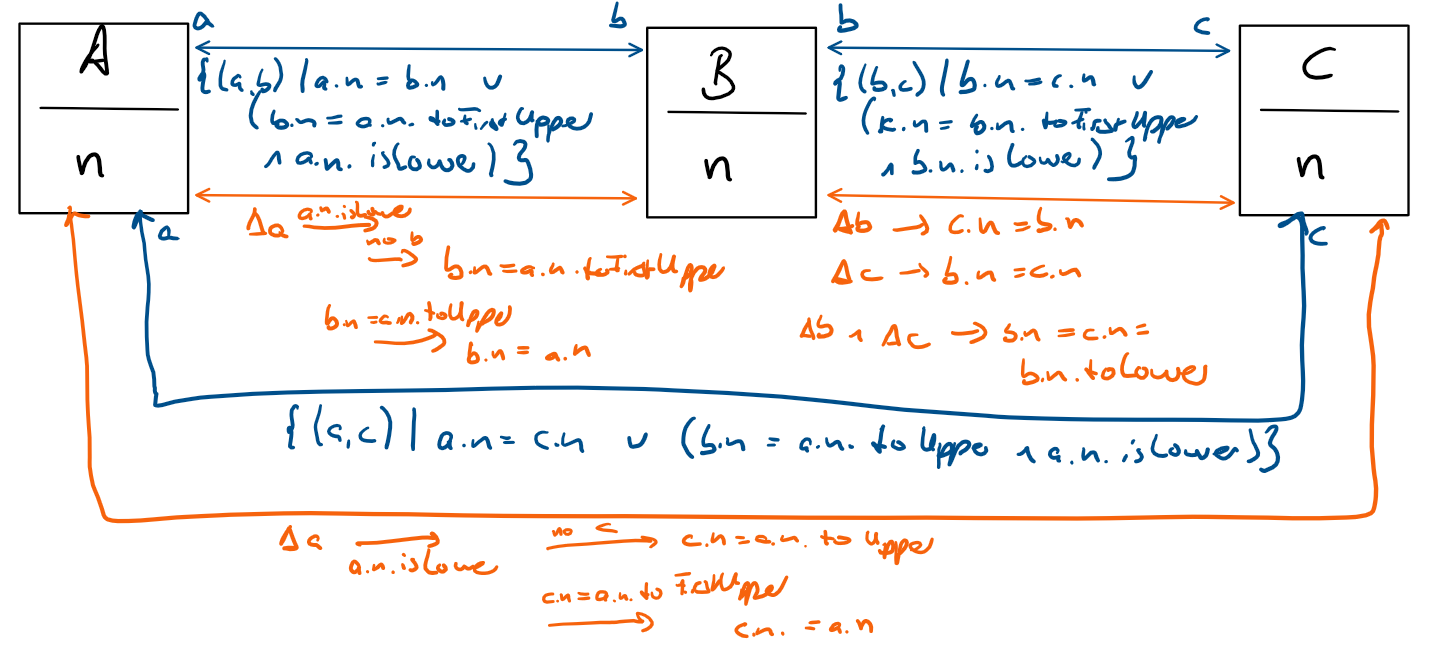
\includegraphics[width=\textwidth]{figures/correctness/formal/monotony_counterexample.png}
    \caption{Counterexample for monotony}
    \label{fig:formal:monotonycounterexample}
\end{figure}

One could now argue that there are binary relations in the example, which may never be fulfilled at all. We will later discuss how far relations that cannot be fulfilled should be restricted. However, in general, this is wanted behavior, because in general it may be necessary that transformations produce intermediate states that are not yet consistent with each other. Otherwise this would means that each transformation is always able to directly deliver a state that is consistent to all other relations, which is especially not possible, because other transformations may add further information to the models. More precisely, a relation may consider a model consistent to all other models that contain any additional information not affected by the transformation. For example, a UML class model may be considered consistent to all Java models with any implementation of the specified methods, thus to an infinite number of models. Now saying that it should not be allowed that the transformation selects one with an empty implementation because that is not consistent to another relations induced by another transformation, such as the relationship to a component model, does not make any sense. Thus having those relation elements that may be considered locally consistent but will never occur in a globally consistent tuple of models does not make sense.
In the example, we can see that such an inconsistent intermediate state is passed through and afterwards a consistent tuple of models is reached if not requiring monotony.
In consequence, requiring monotony from transformations is a too strict requirement, because it is necessary to run through states that may be changed later on.

\begin{theorem}
    An application function for monotone transformations either returns a consistent model or produce a sequence of CPRs returning delta that return models of always growing size (i.e. it diverges).
\end{theorem}


\paragraph{Divergence cannot be avoided}

There are rather equal network, one that terminates after a long time and one that never terminates. 
Consider the example. The relations are defined in a way such that for any allocation for any of them a consistent tuple of models can be found. However, the transformations are not able to find it because they make "bad" choices from a set of choices that are conflicting. 
This can be seen in the example in \autoref{fig:formal:divergenceexample}.

\begin{figure}
    \centering
    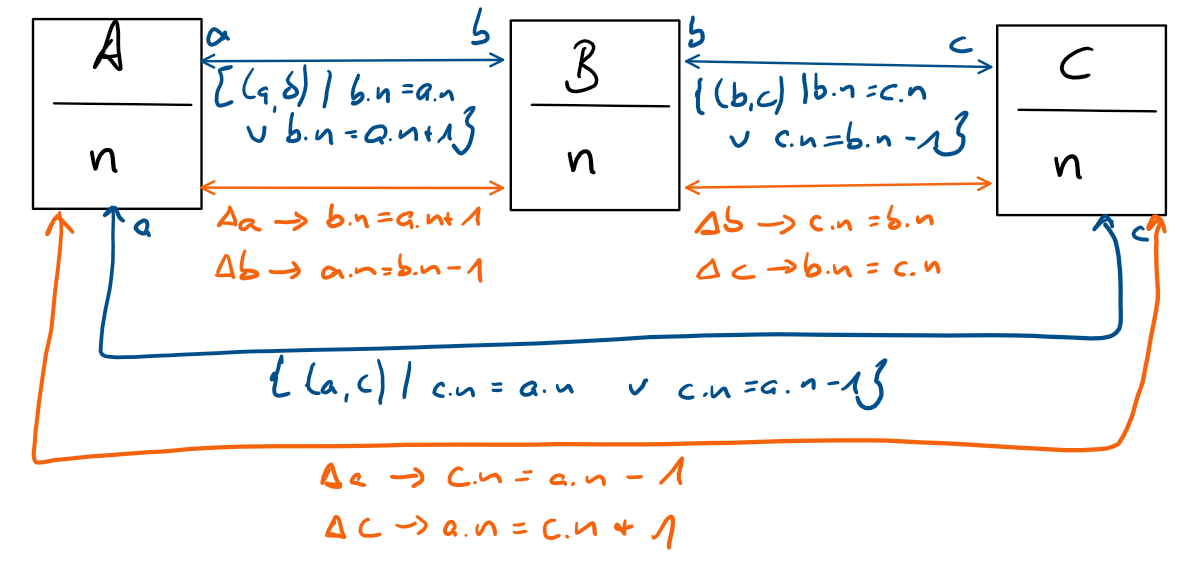
\includegraphics[width=\textwidth]{figures/correctness/formal/divergence_example.png}
    \caption{Example for divergence}
    \label{fig:formal:divergenceexample}
\end{figure}

Thus, systematically avoiding divergence is not possible. 



\paragraph{Detecting Alternation / Divergence}

In consequence, we propose to dynamically deal with alternation / divergence.
To detect alternations, the execution can simply track if a state way already processed. Apart from spatial problems, this does always work.
Finding divergence is not that easy, because it is generally not possible to define an upper bound for the number of executions of a single transformation.
Consider the example in \autoref{fig:formal:noupperboundexample}.

\begin{figure}
    \centering
    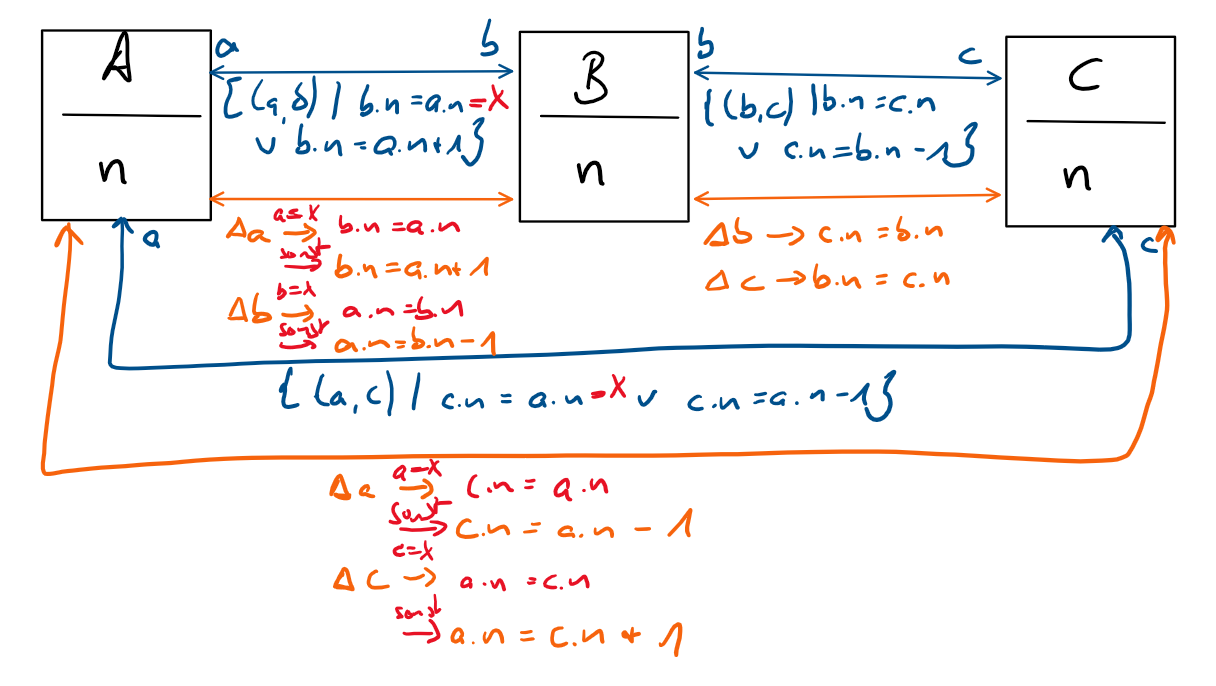
\includegraphics[width=\textwidth]{figures/correctness/formal/no_upper_bound_example.png}
    \caption{Example for no upper bound}
    \label{fig:formal:noupperboundexample}
\end{figure}

Depending on the value X, the transformations have to be executed X times to result in a consistent state. This value can be arbitrarily chosen, thus an arbitrary number of executions may be necessary to terminate in a consistent state.

From an engineering perspective, this is still unwanted behavior. We claim that a transformation network that takes thousands of executions of the same transformation to find a consistent state works not as expected and if running into a failure would expose severe problems to find the reasons for that failures.
Thus, we propose to simply abort the execution after some time to be sure not to run in an endless loop.

Finally, this problem is comparable to ordinary programming, because there the same situations regarding alternation and divergence can occur that result in non-termination of a program.
As we all know, it is impossible to systematically avoid that, but just possible to carefully develop the program and apply best practices to avoid such situations.

In the following, we propose measures to reduce the number of cases in which problematic cases can occur.
In a case study, we will see that using such measures already resolves most of the problems that can occur.
Additionally, we propose an orchestration strategy that improves the possibility to find errors in case something goes wrong.

\textbf{Central insight:} Alternation / Divergence cannot be avoided systematically (like in ordinary programming), if not restricting transformations in a way that may not be reasonable.




\subsection{Reducing Conservativeness of the Application Function}

Goal: Find a solution in as many cases as possible, abort in the others (conservatively). There are two approaches to achieve that: 
1. Reduce the number of cases in which there is no solution by adding assumptions to the relations and transformations (restrict input of app function)
2. Improve the ability to find a solution if it exists (improve capabilities of app function)
Secondary goal: In cases, in which no solution is found, support the user in understanding why no solution was found.


Regarding 1: Reduce problematic cases


1. reduce cases in which there is no such solution
1.1. On relation level: Only sets, so analysis possible.
Ensure that relations are defined in a way such that they do not allow a locally correct set of CPRs that has no APP solution. If there is a pair of models (or elements of a fine-grained relation) in a relation, a CPR may return it. But if there is no consistent tuple of models containing these two, it does not make any sense to consider these elements (even worse, if we have monotony, adding these elements makes the network unsolvable). For that reason, we need compatibility. Avoids both alternation and divergence
1.2. On transformation level: Hard to perform analyses
Require monotony to avoid alternation
Give some example why divergence cannot easily be avoided, thus terminate at some point
2. find the solution in as many cases as possible -> reasonable orchestration strategy
Focus on engineering solution 


Thus, there arise two questions:
- Although theoretically easy, how to practically define a CPR that is synchronizing?
- How to define an APP function and which requirements does that impose?




\section{Notions of Correctness}

\todo{Start with this without the formalization and use informal terms to motivate the definitions.}
\mnote{Correctness implicitly covered by definitions}
\textcite{stevens2010sosym} proposes an explicit notion of \emph{correctness} for transformations. This is based on the fact that her definition of a transformation does only specify that for two given model, which may be inconsistent because one was modified, an update of the other model is returned.
The requirement that the originally modified model and the one returned by the transformation have to conform to some consistency relations is specified externally as a notion of \emph{correctness}.
We directly relate a consistency preservation rule that restores consistency to an according consistency relation, thus a consistency preservation rule that follows our definition is correct by construction in terms of the correctness definition by \citeauthor{stevens2010sosym}.
The same applies to the consistency preservation application function, which we consider \emph{correct} if it fulfills its definition, as that definition already covers all requirements to that function.

\mnote{Different notions of correctness}
In general, correctness can be considered in two ways: First, an artifact may be correct if it simply follows its definition.
While for consistency relations, changes and the generic \modellevelconsistencypreservationrule generalization function correctness can be canonically achieved, this is not that simple for a consistency preservation rule and the consistency preservation application function, as they have to fulfill some constraints with respect to consistency relations they rely on.
Second, an artifact may be correct if it fulfills some, maybe only implicitly known specification. For example, a consistency relation between UML and Java may only be considered correct if it fulfills some \enquote{natural} notion of consistency, as people know how elements have to be related because they represent similar things, such as classes, or because a standard like the UML~\cite{uml} prescribes that.

\mnote{Correctness regarding global specifications}
In this work we do not consider the latter correctness notion with respect to external, maybe not formally specified artifacts, which is part of separate research on validation.
However, when considering consistency of multiple models it may be standing to reason that a modular specification of consistency and its preservation has to be correct with regards to some global, monolithic specification. More precisely, there may be a multiary relation putting several metamodels into relation, which the developers at least implicitly know, and a set of binary relations somehow has to respect that multiary relation, i.e., be \emph{correct} with respect to that relation.
The same can be imagines for consistency preservation. One may define a multidirectional transformation for a multiary relation, taking a tuple of changes to consistent models and retuning a new tuple of changes, which applied to the models delivers a consistent set of models again. In fact, this would be a realization of the behavior of the consistency preservation application function without relying on modular \modellevelconsistencypreservationrules.

\mnote{Drawbacks of global specification notions}
Considering consistency this way has two drawbacks:
\begin{description}
    \item[Validation Artifacts:] The artifacts to check correctness against, i.e., the global, multiary consistency relation as well as an appropriate multidirectional transformation, do usually not exist. If they existed, they could directly be used to preserve consistency. Thus is impossible to validate a set of consistency relations and preservation rules against such a global specification.
    \item[Modular Knowledge:] This notion of correctness requires that the developers have some global knowledge that represents a monolithic, multiary consistency relation and their preservation rules. Usually, this will not be the case, so there is even no implicit notion of the necessary artifacts to validate the modular specifications against, not to be mention an explicit representation.
\end{description}

\todo{Add an image for that relation}








Two levels of correctness:
\begin{enumerate}
    \item Local correctness: a consistency relation is correct to the global relation and the CPR is to the relation, i.e. given two models and changes in them, the transformation can produce a change that restores consistency regarding the global consistency relation of these two models (i.e. there are some other models with which these two models would be consistent regarding the global specification) --> a network is locally correct, if this property is fulfilled
    \item Global correctness: the binary relations together are equal to the global one and the execution function is able to find consistency models after a change to initially consistent models --> network is globally correct, if this property is fulfilled
\end{enumerate}
Potentiell ist lokale Korrektheit (zumindest einer CPR zu ihrer CR per Konstruktion) herstellbar -- das war auch das Ergebnis bisheriger Studien --, eventuell auch von einer CR zu einer globalen CR, obwohl die ja eigentlich meist nicht existiert, daher nehmen wir das als gegeben an.
Dann zeigen, dass die globale Beziehung der Relationen nicht äquivalent ist zu den einzelnen lokalen, daher kommt hier zusätzliche Komplexität rein (Kompatibilitätsbegriff).
Final muss noch die Ausführungsfunktion korrekt sein, hier aber Problem der Turing-Vollständigkeit. 
Daher Einschränkungen an Transformationen finden bzw. ingenieurmäßige Ausführungsreihenfolge festlegen, die möglichst oft richtige Lösungen findet und sonst konservativ mit einem Fehler terminiert.


\textbf{On top of ordinary bx correctness:}
\begin{itemize}
    \item Transformations need to be synchronizing
    \item Consistency relations need to fulfill a notion of correctness
    \item Exkurs:
    \begin{itemize}
    \item Is compatibility a subclass of correctness? Is every correct set of relations compatible as well?
    \item Problematisch: unser Konsistenzbegriff für Relationen (feingranulare Relationen) schließt keine Modelle aus, der Konsistenzbegriff hier aber schon. Wie realisiere ich die feingranularen Relationen, die dafür sorgen, dass nur genau ein Tupel von Modellen konsistent ist?
    \item Wir müssen bei der Ableitung unseres Kompatibilitätsbegriffes erklären, dass bei uns der vollständige Ausschluss bestimmter Modelle nicht Teil einer feingranularen Konsistenzrelation sein darf, sondern Teil einer weiteren Spezifikation, die angibt, welche Modelle überhaupt valide sind. Denn so ist es in Transformationssprachen tatsächlich auch.
    \end{itemize}
    \item Execution function needs to be defined, which potentially induces requirements to the transformations.
\end{itemize}


Trivialisierung des Problems:
\begin{itemize}
    \item Ohne weitere Annahmen ist das immer dadurch erreichbar, dass die Transformationen einen beliebigen anderen Zustand der Modelle produzieren. Im einfachsten Fall liefert jede Transformation immer die gleichen konsistenten Modelle zurück, unabhängig von der Änderung. Dann ist der Endzustand der Modelle nach der Ausführung des Netzwerks immer der gleiche.
    \item Das ist im allgemeinen aber nicht Fall. Letztendlich trifft jede Transformation lokale Entscheidungen. Beispielsweise könnte jede einzelne Transformation gegeben eine beliebige Änderung immer dieselben Modelle (bzw. Änderungen die dazu führen) zurückliefern (im trivialsten Fall leere Modelle). Dann erfüllt jede Transformation ihre Korrektheitseigenschaft bzgl. ihrer Relation, aber das Netzwerk muss nicht korrekt sein, da bspw. T(A,B) und T(B,C) sich immer für verschiedene Instanzen von B entscheiden. Es gäbe somit nie eine konsistente Lösung für eine beliebige Ausführungsreihenfolge der Transformationen, auch wenn die Relationen das erlauben würden.
    \item Beispiel mit Namen, wo eine Transformation immer den großen Namen zurückliefert, die andere immer den kleinen. T(A,B) bildet A auf gleiches B ab und beide auf kleine Schreibweise, obwohl beide erlaubt sind. Erzeuge A="a", dadurch B="a". T(B,C) bildet B auf C ab und beide auf große Schreibweise, obwohl beide erlaubt sind. Somit macht sie das zu B="A" und C="A". Nun wird T(A,B) wieder beide klein machen usw. Allerdings wäre eine insgesamt valide Lösung einfach alle groß oder alle klein zu machen, aber die Transformationen finden diesen Zustand nicht. 
    \item Allgemeiner ist zu sagen, dass ein Transformationsnetzwerk eine Turing-Maschine emulieren kann. \todo{Nachweisen!}
    Im allgemeinen terminiert das Netzwerk somit nicht, schlimmer noch, es ist unentscheidbar, ob das Netzwerk hält (siehe Halteproblem).
    \item Dies zeigt bereits, dass keine Ausführungsfunktion definiert werden kann, die immer ein konsistentes Ergebnis liefert.
    \item Wir versuchen daher Annahmen an Transformationen zu finden, um diese Fälle auszuschließen bzw. systematisch zu verringern. 
    \item Außerdem möchten wir eine Ausführungsfunktion haben, die ein konsistentes Ergebnis liefert oder einen Fehler, denn es muss nicht immer eine korrekte Lösung geben. Ziel ist es dann die Anzahl der Fälle, in denen sie einen Fehler zurückgibt, zu reduzieren.
\end{itemize}

Zielsetzung:
\begin{itemize}
    \item Korrekte Anwendungsfunktion finden (in bestehenden Arbeiten~\cite{stevens2017a}) auch "Resolution" genannt (formal definieren!):
    \item Welche Anforderungen müssen wir dafür an die Transformationen stellen, damit solch eine Funktion definiert werden kann?
    \item Wir bezeichnen das Transformationsnetzwerk, in dem eine Transformation eingesetzt wird, als "Kontext"
    \item Welche dieser Eigenschaften kann die einzelne Transformation (ohne Kenntnis der anderen) erfüllen und für welche muss der Kontext (d.h. die anderen Transformationen) bekannt sein?
    \item $\Rightarrow$ Interesse an "kontextfreien" Eigenschaften (lassen sich ohne Kenntnis der anderen Transformationen sicherstellen -> Wiederverwendbarkeit) und "kontextsensitiven" Eigenschaften (Erfüllung der Eigenschaft nur durch Kenntnis über das Transformationsnetzwerk möglich)
    \item Kontextfreie Eigenschaften involvieren solche, die wir eh schon von Transformationen kennen (Korrektheit einer Transformation, Hippokratie etc.) und solche, die dadurch zustande kommen, dass man weiß, dass diese Transformation in einem Netzwerk eingesetzt werden soll.
    \item Zielsetzungsoptionen:
    \begin{itemize}
        \item Wir schränken die Transformationen so ein, dass es immer mindestens eine Ausführungsreihenfolge der Transformationen gibt, sodass für jede beliebige Änderung ein konsistentes Ergebnis durch Anwenden der Transformationen gefunden werden kann
        \item Wir akzeptieren, dass es Änderungen gibt, für die das Netzwerk kein konsistentes Ergebnis produzieren kann. Dann muss das Netzwerk (mindestens) in diesen Fällen mit einer Fehlermeldung terminieren.
        \item Eine Option ist, dass das Netzwerk dieses Verhalten nur approximiert bzw. approximieren kann, dann muss es sich konservativ verhalten, d.h. im Fall, dass es keine Lösung gibt, auf jeden Fall eine Fehlermeldung geben, und im Fall, in dem es eine Lösung gibt, diese bestenfalls finden oder ausgeben, dass es keine finden kann (d.h. keine False Positives bzw. Nicht-Terminierung). Ziel ist es dann den Grad der Konservativität zu minimieren.
    \end{itemize}
    \item Lösungsoptionen (Grad der Einschränkung an die Transformationen):
    \begin{itemize}
        \item Hohe Einschränkung: Jede beliebige Reihenfolge von ausgeführten Transformationen führt letztendlich zu einem korrekten Ergebnis (Fixpunktiteration -- Allquantifizierung) -- Hippokratie-Eigenschaft sorgt dafür, dass keine Transformation wieder etwas ändert, wenn Konsistenz bereits hergestellt ist.
        Diese Eigenschaft ist in der Praxis möglicherweise zu strikt, da sie sehr starke Anforderungen an die Transformationen stellen müsste. Dafür wäre aber die Anwendungsfunktion trivial.
        \item Mittlere Einschränkung: Es gibt eine Reihenfolge von ausgeführten Transformationen für jede Änderung die terminiert (Existenzquantifizierung) und die Ausführungsfunktion findet diese Reihenfolge.
        Utopisch, dass die Anwendungsfunktion aus (potentiell sehr mächtigen) Transformationen die richtige Reihenfolge errechnen kann. Dafür aber (möglicherweise) weniger Anforderungen an die Transformationen (zumindest nicht mehr Anforderungen, denn die Allquantifzierung induziert die Existenzquantifizierung). Eine Funktion könnte dann zumindest nach best-effort versuchen, die richtige Reihenfolge zu finden und konservativ abbrechen, wenn sie diese nicht finden kann (also entweder konsistent terminieren oder terminieren mit der Aussage, dass es entweder keine solche Reihenfolge gibt -- bei relaxierten Anforderungen -- oder dass es sie nicht finden kann).  
        \item Geringe Einschränkung: Es gibt potentiell keine Reihenfolge der Transformationen, die bei einer Änderung zu einer konsistenten Lösung kommt. Hier müsste die Ausführungsfunktion entsprechend einen Fehler ausgeben.
        \item Bestehende Arbeiten (\cite{stevens2017a}) schlagen auch vor eine Baumstruktur zu berechnen (Spannbaum), in dem nur entlang der Baumkanten die Transformationen ausgeführt werden. Dies ist jedoch eine starke Einschränkung daran, was die Transformationen ausdrücken können. Betrachtet man beispielsweise PCM, UML und Java, und hat eine Änderung in PCM. Dann könnte der Spannbaum entweder PCM -> UML -> Java sein, oder PCM -> UML + PCM -> Java. In ersterem Fall würde Verhaltensbeschreibung, die von PCM nach Java übertragen, aber in UML nicht dargestellt wird, nicht übertragen. Im zweiten Fall würde zusätzliche Information zwischen UML und Java nicht propagiert (Beispiel?) --> Hier sollte auf das Properties-Kapitel verwiesen werden, wo diese "Bottlenecks" erklärt sein sollten, inklusive einem Beispiel, die allgemein Baumstrukturen für Transformationsnetwerke ausschließen.
    \end{itemize}
    \item Dies setzt voraus, dass die Transformationen und die Anwendungsfunktion mit jeder beliebigen Nutzer-Änderung umgehen kann. Man kann jedoch auch verlangen, dass die Anwendungsfunktion genau dann, wenn es überhaupt eine Ausführungsreihenfolge gibt, diese findet, und sonst einen Fehler ausgibt.
    \item \textbf{Wichtig:} Im Allgemeinen kann eine Ausführungsfunktion keine terminierende Reihenfolge berechnen, da die Transformationen Turing-vollständig sind und deshalb die Frage, welche Reihenfolge zu einer Terminierung führt, unentscheidbar ist (Halteproblem). Daher können wir nur einen konservativen Algorithmus angeben, der ein sinnvolles Abbruchkriterium definiert, mit dem die Ausführung beendet wird, auch wenn potentiell eine Lösung hätte gefunden werden können. Die Fragestellung ist also, wie die Ausführungsfunktion aussehen muss, damit sie in möglichst vielen Fällen, in denen es eine terminierenden Reihenfolge gibt, diese auch findet. Insbesondere lässt sich somit keine geschlossene Form für die Ausführungsfunktion angeben, sondern nur ein Algorithmus, der zur Laufzeit eine Reihenfolge (dynamisch) festlegt.
\end{itemize}

Problemraum:
\begin{itemize}
    \item Ziel ist, dass ein Netzwerk von Transformationen nach einer Änderung in einem konsistenten Zustand terminiert. D.h. Korrektheit stellt Anforderungen an \emph{Terminierung}, sowie den \emph{Zustand} bei Terminierung.
    \item Folgende Abweichungen davon können auftreten:
    \begin{enumerate}
        \item Nicht-Terminierung: Das Netzwerk terminiert nicht. Das bedeutet im Prinzip, dass die Ausführungsfunktion (bzw. der Laufzeit-Algorithmus, der die Funktion dynamisch emuliert) nicht \emph{sound} ist. Soundness der Ausführungsfunktion setzt voraus, dass die berechnet Aufrufsequenz endlich ist. Wenn die Ausführung nicht terminiert, bedeutet das, dass entweder die gleichen Zustände mehrfach durchlaufen werden oder eine Sequenz unendlich vieler Zustände produziert wird. Denn wenn beides nicht der Fall ist, gibt es eine endliche Sequenz unterschiedlicher Zustände, d.h. Terminierung. Das bedeutet, dass es folgende zwei Möglichkeiten gibt:
        \begin{itemize}
            \item Alternierung: Die gleichen Zustände werden mehrfach durchlaufen.
            \item Divergenz: Es werden unendlich viele Zustände produziert.
        \end{itemize}
        \item Inkonsistente Terminierung: Die Ausführungsfunktion bzw. der Algorithmus beendet die Ausführung, aber in einem inkonsistenten Zustand. Hier lassen sich ebenfalls wieder zwei Fälle unterscheiden.
        \begin{itemize}
            \item Unerkannte Inkonsistenz: Der Algorithmus terminiert und denkt, der Zielzustand wäre konsistent. Dies bedeutet aber direkt, dass nicht alle Konsistenzrelationen erfüllt sind, was, zumindest in der Theorie, einfach zu prüfen wäre (entweder durch Prüfung der Relationen oder durch Ausführung der hippokratischen Transformationen, die alle nichts tun dürften)
            \item Erkannte Inkonsistenz: Der Algorithmus terminiert, wissend dass die Lösung nicht konsistent ist. Dies kann entweder sein, weil eine Transformation für zwei Modelle in einem inkonsistenten Zustand nicht mehr anwendbar ist, oder weil irgendein anderes Abbruchkriterium erreicht ist.
        \end{itemize}
    \end{enumerate}
\end{itemize}

Annahmen:
\begin{itemize}
    \item Nutzeränderungen dürfen nicht rückgängig gemacht werden.
    \item Nutzeränderungen lassen sich so feingranular zerlegen, dass, falls durch die Erzeugung/Änderung eine Konsistenzrelation verletzt wird, es in jeder unabhängigen Teilmenge von Konsistenzrelationen eine verletzte Konsistenzrelation gibt, für die die geänderten Elemente einem Condition Elemente entsprechen, es also insbesondere keine Teilmenge der geänderten Element gibt, die bereits dieses Condition Element sind. Ansonsten ist durch unsere Kompatibilitäts-Definition nicht sichergestellt, dass eine konsistente Modellmenge gefunden werden kann.
\end{itemize}

Voraussetzungen:
\begin{itemize}
    \item Relationen müssen korrekt sein, d.h. sie müssen bzgl. einer globalen (meist eher implizit bekannten) n-ären Relation zwischen allen Modellen identisch sein. Eine n-äre Relation lässt sich nicht immer zerlegen (siehe Stevens), aber wir nehmen das an.
    \item Die einzelne Transformation muss bzgl. ihrer Relation korrekt sein, d.h. sie muss bei Änderungen in beiden Modellen ein zur Relation konsistentes Modell liefern.
\end{itemize}

Ebenen der Korrektheit:
\begin{itemize}
    \item Relationen müssen korrekt sein, d.h. gegeben eine Nutzeränderung muss es überhaupt möglich sein eine konsistente Menge an Modellen zu finden. Wenn Transformationen etwas beliebigen tun dürfen geht das immer. Wir nehmen an, dass eine Nutzeränderung nicht rückgängig gemacht werden soll (bzw. wenn sie rückgängig gemacht werden würde eigentlich die Änderung invalide war, d.h. keine Konsistenz im Netzwerk hergestellt werden kann). Daher sind Relationen nur korrekt, wenn für fixierte Elemente, die durch eine Nutzeränderung entstehen können, eine Modellmenge abgeleitet werden kann, die bzgl. der Relationen konsistent ist. D.h. gegeben einige Elemente muss es eine Modellmenge geben, die in allen Relationen liegt und die diese Elemente enthält (-> Kompatibilitätsbegriff). Wir betrachten in Kapitel ?, wie man Kompatibilität präzise definieren und feststellen/garantieren kann.\\
    Resultat: Gegeben eine Änderung ist es möglich eine Transformation anzugeben, die aus der Änderung ein konsistentes Modell produziert.
    \item Einzelne Transformationen müssen korrekt sein: Wir fordern Korrektheit der Transformation sowieso. Allerdings machen in einem Netzwerk verschiedene Transformationen Änderungen an allen Modellen, d.h. wir müssen nicht den "normalen" Transformationsfall unterstützen, dass Deltas in einem Modell ins andere übertragen werden, um Konsistenz herzustellen, sondern die Transformationen müssen \emph{synchronisierend} sein, also Deltas in beiden Modelle annehmen und dann Konsistenz herstellen. Wir definieren diese Synchronisationseigenschaft und betrachten in Kapitel ?, welcher zusätzlichen Anforderungen sich dadurch bzgl. EMOF-Modellen ergeben. Der Input sind Deltas in zwei Modellen, und einzelne Deltas sind potentiell als "authoritative" definiert, was bedeutet, dass die erzeugten/geänderten Elemente nicht noch einmal geändert/gelöscht werden dürfen. Das realisiert die Anforderung, dass Nutzeränderungen nicht rückgängig gemacht werden dürfen. \\
    Resultat: Gegeben Änderungen in zwei Modellen (mit potentiell authoritativen Änderungen) gibt die Transformation ein konsistentes (bzgl. der Konsistenzrelation) Modellpaar zurück. 
    \item Korrektheit der Anwendungsfunktion: Die Anwendungsfunktion muss die Transformationen in einer 
\end{itemize}

Annahme an Transformationen:
\begin{itemize}
    \item Muss eine Transformation mit jedem beliebigen Delta umgehen können müssen? Eine Einschränkung auf Monotonie würde dies verhindern. Bzw. wir müssten zeigen, dass es Konsistenzrelationen gibt, die unter der Anforderung an Monotonie nicht wiederhergestellt werden können. Bspw. fügt eine andere Transformation 3 Elemente hinzu, wo zwei mit dem anderen entsprechend der Konsistenzrelationen korrelieren und somit keine Witness-Struktur aufgebaut werden kann, die Konsistenz beweist. Das lässt sich durch Hinzufügen weiterer Elemente potentiell nicht auflösen (siehe Beispiele im SoSym-Paper).
\end{itemize}

Notwendigkeit Transformationen oder Anwendungsfunktion einzuschränken:
\begin{itemize}
    \item Zeigen, dass es Beispiele gibt, in denen es keine einzige Ausführungsreihenfolge gibt (All-Quantifizierung), die zu einem konsistenten Ergebnis führt:
    \item Zeigen, dass es Beispiele gibt, in denen es unabhängig von der Ausführungsreihenfolge immer zu einer Alternierung kommt
    \item Zeigen, dass es Beispiele gibt, in denen es unabhängig von der Ausführungsreihenfolge immer zu einer Divergenz kommt.
    \item Die Beispiele sollten zeigen, dass wir keine Einschränkungen an die Transformationen machen können, was das Problem aushebelt. D.h. egal welche Einschränkungen ich an die Transformationen definiere, es lassen sich immer Beispiele konstruieren, in denen es keine Ausführungsreihenfolge gibt, in denen sie terminieren.
    \item Mathematisch zeigen, dass Alternierung und Divergenz die einzigen Probleme sind. D.h. wenn nicht der gleiche Zustand mehrmals durchlaufen wird (Alternierung) und es nicht unendlich viele Zustände gibt (Divergenz), dann ist die Folge endlich.
    \item Außerdem mathematisch die Abbildung von Transformationen auf Turing-Maschinen zeigen und damit ableiten, dass allgemeine Netzwerke erstmal nicht terminieren müssen (Abbildung auf Halteproblem)
\end{itemize}

Zielsetzung die Zweite:
\begin{itemize}
    \item Wir definieren möglichst minimale Beschränkungen, die dazu führen, dass das Netzwerk terminiert. D.h. es terminiert entweder konsistent oder es terminiert mit einem Fehler, der sagt, dass entweder keine Konsistenz hergestellt werden kann (es gibt keine Ausführungsreihenfolge der Transformationen, die zu Konsistenz führt) oder dass die Anwendungsfunktion nicht in der Lage war eine passende Ausführungsreihenfolge zu finden (Konservativität)
    \item Zwei Arten von Beschränkungen
    \begin{itemize}
        \item Beschränkungen an die Transformationen, die dazu führen, dass es in mehr Fällen mindestens eine Ausführungsreihenfolge gibt, in der das Netzwerk konsistent terminiert
        \item Beschränkungen an die Ausführungsfunktion, sodass die Ausführung auf jeden Fall terminiert, wenn auch konservativ, d.h. mit Fehler, obwohl es eine korrekte Lösung gegeben hätte.
    \end{itemize}
\end{itemize}



Exkurs: Menge (konsistenter) Modelle bildet keinen topologischen Raum
\begin{itemize}
    \item Topologischer Raum besteht aus Grundmenge und Mengensystem von Teilmengen mit den Eigenschaften, dass die Grundmenge offen ist, der Schnitt endlich vieler Mengen offen und die Vereinigung beliebig vieler Mengen offen ist. 
    \item Die Grundmenge wäre die Menge aller Modellelemente
    \item Diese Menge ist normalweise offen, da z.B. für ein Element mit einem String-Attributwert immer noch das Element mit dem gleichen String-Attributwert plus einem weiteren Symbol in der Menge liegt (und man die Ordnung in der Menge entsprechend definiert). Dass ein Metamodell möglicherweise Einschränkungen definiert und dann im schlimmsten Fall nur ein einziges Modell valide ist, lassen wir hier außen vor.
    \item Betrachten wir nun eine Topologie auf dieser Menge, also ein Mengensystem aus konsistenten Modellen. Leider ist jedoch der Schnitt zweier konsistenter Modelle nicht zwangsläufig konsistent. Insbesondere sind diese Mengen auch nicht offen, da sie die abgeschlossene Menge darstellen, die genau ein Modell beschreiben. 
    \item Somit lässt sich die Definition von Topologien hier nicht anwenden.
\end{itemize}

\todo{Überlegen, wo hier die Definition von (undirektionalen Relationen) rein muss.}
Präzisere Eigenschaften:
\begin{itemize} 
    \item Synchronisationseigenschaft: Eine Transformation kann mit Änderungen an mehreren Modellen umgehen, d.h. gegeben zwei konsistente Modelle + Änderungen an beiden resultiert in zwei Modellen, die konsistent bzgl. der Relation(en) zwischen den Metamodellen sind
    \item 
\end{itemize}  




\begin{itemize}
    \item Kompatibilität entsprechend Modularisierungsebene
    \item Synchronisation auf Operationalisierungsebene: Abwägen, dass eine Transformation verschiedene Zustände sehen könnte, auf denen sie ausgeführt wird. Aber letztendlich muss sie damit klarkommen, dass zwei Modelle geändert wurden. 
\end{itemize}

TODO:
\begin{itemize}
    \item Authoritative Modelle (bzw. eher authoritative Regionen) diskutieren (Verweis Stevens)
\end{itemize}



\section{Local Correctness}

Simple solution: we define a transformation which normatively implies a relation, thus it is correct by construction. From a theoretical perspective this is easy to reach, from a practical it is not.
However, in contrast to our definition of synchronizing transformations, ordinary transformations are only able to process changes in one model and update the other accordingly. Together with the assumption that both models were consistent before does not fit with our scenario, because if one model is modified, the other may be modified as well by another transformation across another path, before a transformation is executed. Thus, both models may have been modified.
We consider the following situation: Models A and B were consistent. Model A was changed an we have the changes at hand. Additionally, B was modified because there were other changes propagated through the network. 
We distinguish all cases of modifications to B that may have violated a consistency relation between A and B (according to our fine-grained consistency notion) and consider what we have to do there (e.g. find-or-create-pattern).
Put empirical analysis here.


\section{Correct APP function}

We make the following approach: Always assume there is a solution and start executing the transformation (for now in any order). Finally, the network has to terminate at a fixed point. We investigate, what the reasons may be that it does not try to avoid them.

These reasons can lie in the relations:
- relations cannot be completely unfulfillable, as the empty models are always consistent, thus there can always be CPRs that result in a consistent set of models
- however, if relations contain pairs that can never be in any consistent model tuple they improve proneness to errors, because a CPR may return that pair, which will never fit to any result of any other transformation. Thus, this should not be allowed -> compatibility

These reasons can also lie in the transformations:
- Transformations can make choices and they make choices that are always incompatible to other (refer to example)

Essentially there are two problems: alternation and divergence



\subsection{Other thought}
If each element occurs in each relation only once (so always 1:1 mappings) and if we have compatibility, then any transformation order would return exactly the one model tuple that fits.
However: In that case we would have confluence, every information must directly be available in B from A without a transitive propagation over C. This is not what we want. So there must in general be more than one option a transformation is fine with that to reflect the information that another transformation may add or change.


\todo{Hippocraticness is not necessary but needs to be discussed}

Goal:
- Find a solution in as much cases as possible, abort in the others (conservatively)
- To do so: reduce cases in which there is no such function
- To do so: ensure that relations are defined in a way such that they do not allow a locally correct set of CPRs that has no APP solution. If there is a pair of models (or elements of a fine-grained relation) in a relation, a CPR may return it. But if there is no consistent tuple of models containing these two, it does not make any sense to consider these elements (even worse, if we have monotony, adding these elements makes the network unsolvable). For that reason, we need compatibility.
- 


\section{A Formalization of Compatibility}

\begin{copiedFrom}{SoSym MPM4CPS}

In this section, we precisely define our notion of consistency, and motivate and formally introduce the term \emph{compatibility}.
We first discuss properties of transformation networks %in comparison to a single transformation 
with an intuitive notion of compatibility, based on considerations in existing work.
We then define consistency based on fine-grained consistency relations and,
finally, derive a compatibility notion from the consistency formalization and its pursued perception.
This serves as our contribution \ref{contrib:formalization}.
%An introduction to properties of transformation networks and especially compatibility of transformations, what compatibility means and how the network influences the possibility to give guarantees regarding compatibility.

%\todoHeiko{Discuss extensional definition of relations / constraints and its relation to intensional definitions}
\subsection{Properties of Transformation Network}
\label{sec:compatibility:networkproperties}

%% Correctness as a property of single, bidirectional transformations
Keeping pairs of models consistent by means of incremental, bidirectional transformations has been well researched in recent years~\cite{stevens2010sosym, etzlstorfer2013a, cleve2019dagstuhl}.
A bidirectional transformation consists of a \emph{relation} that specifies which pairs of models are considered consistent and a pair of directional transformations, denoted as \emph{consistency repair routines}, that take one modified and one originally consistent model and deliver a new model that is consistent to the modified one~\cite{stevens2010sosym}.
Several well-defined properties of such transformations have been identified.
The essential \emph{correctness} property states that a consistency repair routine delivers a result such that the models are actually consistent according to the defined relation~\cite{stevens2010sosym}.
Another important property is \emph{hippocraticness}, which states that a consistency repair routine returns the input model if it was already consistent to the modified one~\cite{stevens2010sosym}.

%%
%% Correctness property of transformation networks, not induced by correctness of single transformations
%%
When we combine several transformations to a network to achieve consistency between multiple models, those properties of the single transformations are still relevant, as each transformations on its own has to be at least correct to work properly in a network of transformations.
However, correctness of the single transformations does not induce correctness of the transformation network.
Taking an arbitrary set of correct transformations and executing them one after another does not necessarily constitute a terminating approach that delivers a result, in which all models are consistent according to the relations of the transformations, because the result of one transformation may violate the relation of another.
It is possible that the approach does either not terminate, because there is a divergence or alternation in values changed or elements created, or terminates in a state that is not consistent regarding the relations of all transformations~\cite{klare2019icmt}.
%Consider the example of $R_{PE}, R_{PR}, R'_{ER}$ in \autoref{fig:motivational_example}. A transformation network in which each transformation adds the corresponding element for an added element, such as a resident for an added person by the transformation of $R_{PR}$.
\todoDiss{Readd}
%Since the execution of one transformation may lead to a violation of the relation of another transformation, executing each transformation only once can easily lead to termination in an inconsistent state.
%In consequence, transformations have to be executed in a fixed point iteration manner, until all relations are fulfilled.
The property of a network to always result in a state in which the models are consistent to all relations of the transformations if they are executed in a specific order, can be seen as a \emph{correctness} property for transformation networks.
In this work, we focus on that correctness property and do not discuss further quality properties of transformation networks, such as \emph{modularity}, \emph{evolvability} and \emph{comprehensibility}~\cite{klare2018docsym}.


%%
%% Correctness considerable at different levels.
%%
A single transformation can only be incorrect in terms of its repair routines, because there are no restrictions regarding its relation that may prevent the repair routine from being able to produce a correct result.
In previous work, however, we identified that transformation networks can be incorrect at different levels~\cite{klare2019icmt}.
Networks can also be incorrect at the level of relations rather than repair routines, because multiple relations can be contradictory, i.e., they can relate elements in different ways such that the relations cannot be fulfilled at the same time.
\todoDiss{Readd}
%This especially concerns the \emph{modularization level}, which considers correctness of the binary relations of a set of bidirectional transformations describing when a set of models is consistent, and the \emph{operationalization level}, which considers correctness of the consistency repair routines in terms of producing models that are correct regarding the relations of all bidirectional transformations.
%For a single transformation, there are no restrictions regarding its relation that may prevent the repair routines from being able to produce a correct result, thus correctness is only considered at the operationalization level. %The correctness definition of \textcite{stevens2010sosym} for a single transformation only concerns the operationalization level, because a single relation is correct by construction. 
% Considering only a single transformation, its relation is correct by definition, at least if there is no external specification against which the relations have to be correct, thus the definition of \textcite{stevens2010sosym} for correctness only considers the consistency repair routines.
%However, in case of a transformation network, the different relations may be contradictory, i.e., elements are related in a different way such that the relations cannot be fulfilled at the same time.
In such a case, the consistency repair routines cannot be result in a state that is consistent according to the relations anymore, thus they may not terminate anymore.
%This is due to the fact that several relations can relate the same elements in a different way, such that they cannot be fulfilled at the same time, i.e. that they are contradictory.
%In such a case, the iteration will not terminate.
We call the relations of such transformations \emph{incompatible}.
%We define this informal notion of compatibility more precisely in the remainder of this section.

%%
%% Compatibility not achievable by construction -> we focus on checking it
%%
In consequence, compatibility of relations is a necessary prerequisite for consistency repair routines to produce correct results in transformation networks.
We also found that correctness of the consistency repair routines can already be achieved by construction, whereas compatibility of the relations cannot be achieved by construction but in the best case be checked for a set of relations.
In this work, we focus on the possibility to check compatibility of the relations of a set of transformations.
In the following, we therefore precisely define the notion of compatibility of relations, which excludes contradictions in relations that can prevent consistency repair routines from fulfilling the relation.

\todo{Example!}

%%
%% Tree topology excludes compatibility
%%
%\subsection{Network Topology Impacts}
Finally, the topology of a transformation network directly influences how prone it is to incompatibilities of its relations.
Contradictions of consistency relations, as exemplified with the relations $R_{PE}, R_{PR}, R'_{ER}$ in \autoref{fig:prologue:three_persons_example}, can only occur if the same classes are related to each other by different (sequences of) transformations in a different way.
For example, in \autoref{fig:prologue:three_persons_example}, each combination of two relations puts the same classes into relation as the third one.
%This can also be a the case if a sequence of transformations introduces this relation, like each combination of two relations in \autoref{fig:motivational_example} relates the same classes as the third relation.
This means that a transformation network, in which each pair of classes is only related by one sequence of transformations, cannot have contradictory relations and is thus inherently compatible.



% \subsection{Consistency by Transformation Networks}

% \begin{itemize}
%     \item Incremental, bidirectional transformations serve as a means for preserving consistency of models by updating one if the other is modified
%     \item Transformations specify the conditions for consistency (consistency relations), as well as how consistency can be restored after modifications (consistency repair)~\cite{stevens2010sosym}
%     \item Consistency between more than two models can be achieved by coupling bidirectional transformations to networks
%     \item Even if the single transformations are correct, i.e. consistency repair produces results that conform to the consistency relations~\cite{stevens2010sosym}, this may not be the case when \emph{independently developed} bidirectional transformations are combined.
%     \item Interoperability problems can occur at the level of consistency relations, i.e. that the relations of the different transformations cannot be fulfilled at the same time, or at the level of consistency repair, i.e. that the repair routines do not terminate in a consistent state or even not at all~\cite{klare2019icmt}
%     \item While \textcite{klare2019icmt} focused on techniques to avoid interoperability issues at the level of consistency repair, in this work we focus on finding interoperability issues of the underlying consistency relations, which we previously defined as \emph{compatibility} issues~\cite{klare2018docsym}.
%     The avoidance of interoperability issues at the relations level is a necessary assumption to avoid issues at the operationalization level.
% \end{itemize}


% \subsection{Network Topology Impacts}

% \begin{itemize}
%     \item Idea: Couple independently developed transformations (refer to running example) to network
%     \item Problem: Trade-off between different properties, depending on the chosen or induced network topology
%     \item Introduce contrary properties \emph{compatibility} and \emph{modularity} (provide only a naive explanation) and shortly refer to evolvability/comprehensibility \cite{klare2018docsym}.
%     \item Explain problems of building tree structures (inherent compatibility) and motivate arbitrary graph structures, providing high modularity, but not giving compatibility guarantees
% \end{itemize}

\subsection{A Fine-grained Notion of Consistency}

A common definition of consistency enumerates consistent pairs of models in a relation~\cite{stevens2010sosym}.
However, for our studies on compatibility, we need a more fine-grained notion of consistency.
Considering transformations languages, such as \qvtr, first, relations are defined at the level of classes and their properties, i.e. how properties of instances of some classes are related to properties of instances of other classes.
Second, they are defined in an \emph{intensional} way, i.e., constraints specify which elements shall be considered consistent, rather than enumerating all consistent instances, known as an \emph{extensional} specification.
Both ways have equal expressiveness and especially each intensional specification can be transformed into an extensional one by enumerating all instances that fulfill the constraints.
Since mathematical statements are easier to make on extensional specifications, we stick to them.
However, we reuse the concept of specifying relations at the level of classes and their properties. % rather than complete models.
This makes it easier to make statements about dependencies between consistency relations.
For example, two fine-grained consistency relations considering completely independent sets of classes cannot interfere, and thus especially do not introduce any compatibility problems, which is not easy to express when considering relations at the level of complete models.
Finally, from such a fine-grained specification, a holistic relation at level of models can always be derived by enumerating all models that fulfill all the fine-grained specifications, thus it does not restrict expressiveness in any way and can be seen as a \emph{compositional approach} for defining consistency.

In the following, we start with introducing a fine-grained notion of consistency relations. % based on such fine-grained consistency relations.
We proceed with considerations on implicit relations, which are induced by a set of consistency relations, such as transitive relations, to finally precisely define a notion of compatibility.

% General notion of consistency consider relations of models. We use a more fine-grained notion based on consistency relations, which requires those relations to be unidirectional, and the notion of consistency to be more complex. The simple notion (model left requires related model right and vice versa) is not applicable, but induced by our fine-grained specification.

% \begin{itemize}
%     \item Instead of considering relations on the metamodel level, we can consider relations on the element level
%     \item Idea: Create a graph of meta elements (meta-classes, attributes, references) containing edges for all relations between elements defined by consistency relations (if there is a rule relating two or more elements, there is an edge between them)
%     \item If this graph of fine-grained relations forms a set of trees, the transformations are compatible (apply definition from previous section), because a change to one element may only be propagated across one path to each of all other elements
%     \item This is what we call \emph{decomposition} that witnesses compatibility.
%     \item We explain this in detail in \autoref{sec:decomposition}.
% \end{itemize}


%\subsection{Compatibility in Transformation Networks}

% As introduced in the previous section, simply put, compatibility in a transformation network means that there are no contradictions in the relations defined by the transformations. That means, there are not restrictions in the relations that prevent another relation from being fulfilled.
% To precisely specify that notion of \emph{compatibility}, the problems associated with it and prove correctness of a strategy to verify compatibility of given relations, we define our notion of consistency in terms of conditions and consistency relations and define the term \emph{compatibility} based on that.


\subsubsection{Consistency}

The first definitions on conditions and consistency relations are based on the work of \textcite[sec. 2.3.2, 4.1.1]{kramer2017a}.
The central idea of the consistency notion is to have consistency relations, which contain pairs of objects and, broadly speaking, requires that if the objects in one side of the pair occur in a model, the others have to occur in another model as well.

\begin{definition}[Condition]
    A condition $\condition{c}{}$ for a class tuple $\classtuple{C}{\condition{c}{}} = \tupled{\class{C}{\condition{c}{},1}, \dots, \class{C}{\condition{c}{},n}}$ is a set of object tuples %$\condition{c}{}$ = \setted{\tupled{\object{o}{1}, \dots, \object{o}{n}}}$ 
    with: 
    \begin{align*}
    \formulaskip &
    \forall \tupled{\object{o}{1}, \dots, \object{o}{n}} \in \condition{c}{}: \forall i \in \setted{1, \dots, n} : \object{o}{i} \in \metamodelinstances{\class{C}{\condition{c}, i}}
    \end{align*}
    An element $\conditionelement{c}{} \in \condition{c}{}$ is called a \emph{condition element}.
    %
    For a set of models $\modelset{m} \in \metamodelinstances{\metamodelset{M}}$ of a metamodel set $\metamodelset{M}$ and %= \setted{\model{m}{1}, \dots, \model{m}{k}}$ 
    a condition element $\conditionelement{c}{}$, % = \tupled{\object{o}{1}, \dots, \object{o}{n}}$ 
    %be a condition element.
    we say that: 
    \begin{align*}
        \formulaskip &
        \modelset{m} \mathtext{contains} \conditionelement{c}{} \equivalentperdefinition
        \exists \model{m}{} \in \modelset{m} : \conditionelement{c}{} \subseteq \model{m}{}
    \end{align*}
\end{definition}

\emph{Conditions} represent object tuples that instantiate the same tuple of classes. They are supposed to occur in models that fulfill a certain condition regarding consistency, i.e., they define the objects that can occur in the previously mentioned pairs of consistency relations, which we specify later.
% \begin{definition}[Condition Element Containment] \label{def:conditionelementcontainment}
%     For a set of metamodels $\metamodelset{M}$, let $\modelset{m} \in \metamodelinstances{\metamodelset{M}}$ %= \setted{\model{m}{1}, \dots, \model{m}{k}}$ 
%     be a set of models and let $\conditionelement{c}{} = \tupled{\object{o}{1}, \dots, \object{o}{n}}$ be a condition element.
%     We say that:
%     \begin{align*}
%         \formulaskip &
%         \modelset{m} \mathtext{contains} c \equivalentperdefinition \\
%         & \formulaskip
%         \exists \model{m}{} \in \modelset{m} : \exists \object{o'}{1}, \dots, \object{o'}{n} \in \model{m}{} : \forall i \in \setted{1, \dots, n} : \object{o}{i} \subseteq \object{o'}{i}
%     \end{align*}
% \end{definition}
We say that a set of models contains a condition element if any of the models contains all the objects within the condition element. %a set of objects, in which the condition is represented. 
%This does not necessarily mean that the objects have to be exactly those of the condition, but may be a superset of them.
%That definition allows to a condition may only specify partial information of an object to match, as, for example, a consistency relation may only relate specific properties of classes instead of the whole classes.
This implies that the metamodel of such a model has to contain all the classes in the class tuple of the condition.

\todoDiss{Call class tuple the "signature" of a relation.}
\begin{definition}[Consistency Relation]
\label{def:consistencyrelation}
    %Let $\metamodel{M}{1}, \metamodel{M}{2}$ be two metamodels. 
    %A consistency relation $\consistencyrelation{CR}{}$ is defined for two class tuples $\classtuple{C}{l,\consistencyrelation{CR}{}}$ and $\classtuple{C}{r,\consistencyrelation{CR}{}}$ 
    %with $\forall \class{C}{l,i} \in \classtuple{C}{l,\consistencyrelation{CR}{}} : \exists \class{C}{} \in \metamodel{M}{1} : \class{C}{l,i} \subseteq \class{C}{}$ and $\forall \class{C}{r,i} \in \classtuple{C}{r,\consistencyrelation{CR}{}} : \exists \class{C}{} \in \metamodel{M}{2} : \class{C}{r,i} \subseteq \class{C}{}$.
    % $\consistencyrelation{CR}{}$ is a set of pairs of condition elements
    % \begin{align*}
    %     \formulaskip
    %     \consistencyrelation{CR} = \setted{\tuple{c}{l} = \tupled{\object{o}{l,1}, \dots, \object{o}{l,n}}, \tuple{c}{r} = \tupled{\object{o}{r,1}, \dots, \object{o}{r,m}}}
    % \end{align*}
    % such that there are induced conditions $\condition{c}{l,\consistencyrelation{CR}{}}, \condition{c}{r,\consistencyrelation{CR}{}}$ 
    % \begin{align*}
    %     \exists 
    % \end{align*}
    Let $\classtuple{C}{l,\consistencyrelation{CR}{}}$ and $\classtuple{C}{r,\consistencyrelation{CR}{}}$ be two class tuples.
    A consistency relation $\consistencyrelation{CR}{}$ is a subset of pairs of condition elements in conditions $\condition{c}{l,\consistencyrelation{CR}{}}, \condition{c}{r,\consistencyrelation{CR}{}}$ with
    $\classtuple{C}{l,\consistencyrelation{CR}{}} = \classtuple{C}{\condition{c}{l,\consistencyrelation{CR}{}}}$ and $\classtuple{C}{r,\consistencyrelation{CR}{}} = \classtuple{C}{\condition{c}{r,\consistencyrelation{CR}{}}}$ :
    \begin{align*}
        \formulaskip & 
        \consistencyrelation{CR}{} \subseteq \condition{c}{l,\consistencyrelation{CR}{}} \times \condition{c}{r,\consistencyrelation{CR}{}}
    \end{align*}
    We call a pair of condition elements %$\consistencyrelationpair{cr}{} 
    $\tupled{\conditionelement{c}{l}, \conditionelement{c}{r}} \in \consistencyrelation{CR}{}$ a \emph{consistency relation pair}. 
    For a set of models $\modelset{m}$ and a consistency relation pair $\tupled{\conditionelement{c}{l}, \conditionelement{c}{r}}$, we say that:
    \begin{align*}
        \formulaskip & 
        \modelset{m} \mathtext{contains} \tupled{\conditionelement{c}{l}, \conditionelement{c}{r}} \equivalentperdefinition \modelset{m} \mathtext{contains} \conditionelement{c}{l} \land \modelset{m} \mathtext{contains} \conditionelement{c}{r}
    \end{align*}
    Without loss of generality, we assume that each condition element of both conditions occurs in at least one consistency relation pair, i.e.
    \begin{align*}
        \formulaskip & 
        \forall \conditionelement{c}{} \in \condition{c}{l} : \exists \tupled{\conditionelement{c}{l}, \conditionelement{c}{r}} \in \consistencyrelation{CR}{} : \conditionelement{c}{} = \conditionelement{c}{l} \\
        &  
        \land \forall \conditionelement{c}{} \in \condition{c}{r} : \exists \tupled{\conditionelement{c}{l}, \conditionelement{c}{r}} \in \consistencyrelation{CR}{} : \conditionelement{c}{} = \conditionelement{c}{r}
    \end{align*}
    % these metamodels is a (possibly infinite) set of pairs of model element tuples $\consistencyrelation{CR} = \{ \bigtupled{\tupled{e_{l1}, \ldots, e_{ln}}, \tupled{e_{r1}, \ldots, e_{rm}}}, \bigtupled{\tupled{f_{l1}, \ldots, f_{ln}}, \tupled{f_{r1}, \ldots, f_{rm}}}, \newline \dots \}$ with the elements of each left tuple $e_{li}, f_{li}, \ldots \in \metamodelinstances{\metamodel{M}}$ and the elements of each right tuple $e_{ri}, f_{ri}, \ldots \in \metamodelinstances{\metamodel{N}}$.
    % A consistency relation denotes that the element tuples have to co-occur or to not occur at all in instances of $\metamodel{M}$ and $\metamodel{N}$ to consider these instances consistent.
\end{definition}

A consistency relation according to \autoref{def:consistencyrelation} is a set of pairs of object tuples, which are supposed to indicate the tuples of objects that are considered consistent with each other, i.e., if a model contains one of the left object tuples occurs in the relation one of the related right object tuples has to occur in a model as well.
It is based on two conditions that define relevant object tuples in each of the two metamodels and defines the ones that are related to each other.
\todo{Metamodels in definition may not be different, so consistency relations within a model can be defined. May be a problem if the class tuples are overlapping, so exclude and discuss that?}

We can now define a notion of consistency for a set of models based on the definition of consistency relations.

\begin{definition}[Consistency] \label{def:consistency}
    %Let $\metamodelset{M} = \setted{ \metamodel{M}{1}, \dots, \metamodel{M}{k} }$ be a set of metamodels and 
    Let $\consistencyrelation{CR}{}$ be a consistency relation % for two of the metamodels in $\metamodelset{M}$.
    %Let 
    and let $\modelset{m} \in \metamodelinstances{\metamodelset{M}}$ %= \setted{ \model{m}{1}, \dots, \model{m}{k} }, \model{m}{i} \in \metamodelinstances{\metamodel{M}{i}}$ 
    be a set of models of the metamodels in $\metamodelset{M}$.
    We say that:
    % \begin{align*}
    %     \formulaskip
    %     & 
    %     \modelset{m} \mathtext{consistent to} \consistencyrelation{CR}{} \equivalentperdefinition \\
    %     & \formulaskip
    %     \forall \tuple{c}{l} \in \condition{c}{l, \consistencyrelation{CR}{}} \mid \modelset{m} \mathtext{contains} \conditionelement{c}{l} : \exists \conditionelement{c}{r} \in \condition{c}{r, \consistencyrelation{CR}{}} : \\
    %     & \formulaskip\formulaskip 
    %     \tupled{\conditionelement{c}{l}, \conditionelement{c}{r}} \in \consistencyrelation{CR}{} \land \modelset{m} \mathtext{contains} \conditionelement{c}{r} \\
    %     & \formulaskip
    %     \land \forall \conditionelement{c}{r} \in \condition{c}{r, \consistencyrelation{CR}{}} \mid \modelset{m} \mathtext{contains} \conditionelement{c}{r} : \exists \conditionelement{c}{l} \in \condition{c}{l, \consistencyrelation{CR}{}} : \\
    %     & \formulaskip\formulaskip 
    %     \tupled{\conditionelement{c}{l}, \conditionelement{c}{r}} \in \consistencyrelation{CR}{} \land \modelset{m} \mathtext{contains} \conditionelement{c}{l}
    % \end{align*}
     \begin{align*}
        \formulaskip
        & 
        \modelset{m} \mathtext{consistent to} \consistencyrelation{CR}{} \equivalentperdefinition \\
        & \formulaskip
        \exists \consistencyrelation{W}{} \subseteq \consistencyrelation{CR}{} : 
        \bigl( \forall \tupled{\conditionelement{c}{l,1}, \conditionelement{c}{r,1}}, \tupled{\conditionelement{c}{l,2}, \conditionelement{c}{r,2}} \in \consistencyrelation{W}{} : \\
        & \formulaskip\formulaskip\formulaskip
        \tupled{\conditionelement{c}{l,1}, \conditionelement{c}{r,1}} = \tupled{\conditionelement{c}{l,2}, \conditionelement{c}{r,2}} \lor 
        ( \conditionelement{c}{l,1} \neq \conditionelement{c}{l,2} \land \conditionelement{c}{r,1} \neq \conditionelement{c}{l,2}) \bigr) \\
        & \formulaskip\formulaskip
        \land \forall \tupled{\conditionelement{c}{l}, \conditionelement{c}{r}} \in  \consistencyrelation{W}{} : \modelset{m} \containsmath \conditionelement{c}{l} \land \modelset{m} \containsmath \conditionelement{c}{r} \\
        & \formulaskip\formulaskip
        \land \forall \conditionelement{c'}{l} \in \condition{c}{l,\consistencyrelation{CR}{}} : \modelset{m} \containsmath \conditionelement{c'}{l} \Rightarrow \conditionelement{c'}{l} \in \condition{c}{l,\consistencyrelation{W}{}}
        % & \formulaskip\formulaskip
        % \land 
        % \forall \conditionelement{c'}{r} \in \condition{c}{r,\consistencyrelation{CR}{}} \mid \modelset{m} \containsmath \conditionelement{c'}{r} : \conditionelement{c'}{r} \in \condition{c}{r,\consistencyrelation{W}{}}
    \end{align*}
    We call such a $\consistencyrelation{W}{}$ a \emph{witness structure} for consistency of $\modelset{m}$ to $\consistencyrelation{CR}{}$, and for all elements $\tupled{\conditionelement{w}{l}, \conditionelement{w}{r}} \in \consistencyrelation{W}{}$, we call $\conditionelement{w}{l}$ and $\conditionelement{w}{r}$ \emph{corresponding to} each other.
    
    For a set of consistency relations $\consistencyrelationset{CR} = \setted{\consistencyrelation{CR}{1}, \consistencyrelation{CR}{2}, \dots}$, we say that:
    \begin{align*}
        \formulaskip &
        \modelset{m} \mathtext{consistent to} \consistencyrelationset{CR} \equivalentperdefinition \\
        & \formulaskip
        \forall \consistencyrelation{CR}{} \in \consistencyrelationset{CR} : \modelset{m} \mathtext{consistent to} \consistencyrelation{CR}{}
    \end{align*}
\end{definition}

\begin{figure}
    \centering
    \newcommand{\hdistance}{20em}
\newcommand{\vdistance}{0.8em}
\newcommand{\internalvdistance}{0.3em}
\newcommand{\classwidth}{6em}
\newcommand{\objectwidth}{6.7em}
\newcommand{\leftshift}{5em}

\begin{tikzpicture}[
    witness/.style={consistency relation, latex-latex},
    witness fault/.style={witness, color=darkred, dashed}
]

% Employee
\umlclassvarwidth{employee}{}{Employee\sameheight}{
name
}{\classwidth}

% Resident
\umlclassvarwidth[, right=\hdistance of employee.north, anchor=north]{resident}{}{Resident\sameheight}{
name
}{\classwidth}

% CONSISTENCY RELATIONS
\draw[consistency relation] (employee.east) -- node[pos=0, above right] {$e$} node[pos=0.5, below, align=center] {
$\begin{aligned}
    \consistencyrelation{CR}{} = \setted{ \tupled{e,r} \mid e.name = r.name \\[-0.4em]
	\lor e.name.toLower = r.name }
\end{aligned}$} node[pos=1, above left] {$r$} (resident.west);

% EXAMPLE 1
% Employee
\umlobjectvarwidth[, below right=2.2*\vdistance and \leftshift of employee.south west, anchor=north west]{instance1_employee}{}{Employee\sameheight}{
	name = "Alice"
}{\objectwidth}
% Resident
\umlobjectvarwidth[, below=2.2*\vdistance of resident.south east, anchor=north east]{instance1_resident}{}{Resident\sameheight}{
	name = "Alice"
}{\objectwidth}

% EXAMPLE 2
% Employee
\umlobjectvarwidth[, below=\vdistance of instance1_employee.south, anchor=north]{instance2_employee}{}{Employee\sameheight}{
	name = "alice"
}{\objectwidth}
% Resident
\umlobjectvarwidth[, below=\vdistance of instance1_resident.south, anchor=north]{instance2_resident}{}{Resident\sameheight}{
	name = "Alice"
}{\objectwidth}


% EXAMPLE 3
% Employee
\umlobjectvarwidth[, below=\vdistance of instance2_employee.south, anchor=north]{instance3_employee1}{}{Employee\sameheight}{
	name = "alice"
}{\objectwidth}
\umlobjectvarwidth[, below=\internalvdistance of instance3_employee1.south, anchor=north]{instance3_employee2}{}{Employee\sameheight}{
	name = "Alice"
}{\objectwidth}
% Resident
\umlobjectvarwidth[, below=\vdistance of instance2_resident.south, anchor=north]{instance3_resident1}{}{Resident\sameheight}{
	name = "alice"
}{\objectwidth}
\umlobjectvarwidth[, below=\internalvdistance of instance3_resident1.south, anchor=north]{instance3_resident2}{}{Resident\sameheight}{
	name = "Alice"
}{\objectwidth}

% EXAMPLE 4
% Employee
\umlobjectvarwidth[, below=\vdistance of instance3_employee2.south, anchor=north]{instance4_employee1}{}{Employee\sameheight}{
	name = "Alice"
}{\objectwidth}
% Resident
\umlobjectvarwidth[, below=\vdistance of instance3_resident2.south, anchor=north]{instance4_resident1}{}{Resident\sameheight}{
	name = "Alice"
}{\objectwidth}
\umlobjectvarwidth[, below=\internalvdistance of instance4_resident1.south, anchor=north]{instance4_resident2}{}{Resident\sameheight}{
	name = "John"
}{\objectwidth}

% EXAMPLE 5
% Resident
\umlobjectvarwidth[, below=\vdistance of instance4_resident2.south, anchor=north]{instance5_resident1}{}{Resident\sameheight}{
	name = "Alice"
}{\objectwidth}
\umlobjectvarwidth[, below=\internalvdistance of instance5_resident1.south, anchor=north]{instance5_resident2}{}{Resident\sameheight}{
	name = "alice"
}{\objectwidth}
% Employee
\umlobjectvarwidth[, left=\hdistance-\leftshift+(\classwidth-\objectwidth) of instance5_resident1.north, anchor=north]{instance5_employee1}{}{Employee\sameheight}{
	name = "alice"
}{\objectwidth}

% EXAMPLE 6
% Resident
\umlobjectvarwidth[, below=\vdistance of instance5_resident2.south, anchor=north]{instance6_resident1}{}{Resident\sameheight}{
	name = "alice"
}{\objectwidth}
% Employee
\umlobjectvarwidth[, left=\hdistance-\leftshift+(\classwidth-\objectwidth) of instance6_resident1.north, anchor=north]{instance6_employee1}{}{Employee\sameheight}{
	name = "alice"
}{\objectwidth}
\umlobjectvarwidth[, below=\internalvdistance of instance6_employee1.south, anchor=north]{instance6_employee2}{}{Employee\sameheight}{
	name = "Alice"
}{\objectwidth}

\node[left=0.5*\leftshift of instance1_employee.west] {\textbf{1.}};
\node[left=0.5*\leftshift of instance2_employee.west] {\textbf{2.}};
\node[left=0.5*\leftshift of instance3_employee1.west] {\textbf{3.}};
\node[left=0.5*\leftshift of instance4_employee1.west] {\textbf{4.}};
\node[left=0.5*\leftshift of instance5_employee1.west] {\textbf{5.}};
\node[left=0.5*\leftshift of instance6_employee1.west] {\textbf{6.}};

\draw ([xshift=-\leftshift,yshift=0.5*\vdistance]instance1_employee.north west) -- ([yshift=0.5*\vdistance]instance1_resident.north east); 
\draw ([xshift=-\leftshift,yshift=0.5*\vdistance]instance2_employee.north west) -- ([yshift=0.5*\vdistance]instance2_resident.north east); 	 
\draw ([xshift=-\leftshift,yshift=0.5*\vdistance]instance3_employee1.north west) -- ([yshift=0.5*\vdistance]instance3_resident1.north east); 	 
\draw ([xshift=-\leftshift,yshift=0.5*\vdistance]instance4_employee1.north west) -- ([yshift=0.5*\vdistance]instance4_resident1.north east); 	 
\draw ([xshift=-\leftshift,yshift=0.5*\vdistance]instance5_employee1.north west) -- ([yshift=0.5*\vdistance]instance5_resident1.north east); 
\draw ([xshift=-\leftshift,yshift=0.5*\vdistance]instance6_employee1.north west) -- ([yshift=0.5*\vdistance]instance6_resident1.north east); 	


% WITNESS STRUCTURE
\draw[witness] (instance1_employee) -- (instance1_resident);
\draw[witness] (instance2_employee) -- (instance2_resident);
\draw[witness] (instance3_employee1) -- (instance3_resident1);
\draw[witness] (instance3_employee2) -- (instance3_resident2);
\draw[witness] (instance4_employee1) -- (instance4_resident1);
\draw[witness fault] (instance5_employee1) -- (instance5_resident1);
\draw[witness fault] (instance5_employee1) -- (instance5_resident2);
\draw[witness fault] (instance6_employee1) -- (instance6_resident1);
\draw[witness fault] (instance6_employee2) -- (instance6_resident1);

\end{tikzpicture}
    \caption{A consistency relation between employee and resident and six example model pairs: model pairs 1--4 being consistent with an appropriate witness structure $\consistencyrelation{W}{}$ shown in blue and model pair 5 and 6 being inconsistent with an inappropriate mapping structure shown in red and dashed.}
    \label{fig:correctness:formal:consistency_example}
\end{figure}

A consistency relation $\consistencyrelation{CR}{}$ relates one condition element at the left side to one or more other condition elements at the right side of the relation.
The definition of consistency ensures that if one condition element $\conditionelement{c}{} \in \condition{c}{l,\consistencyrelation{CR}{}}$ in the left side of the relation occurs in a set of models, exactly one of the condition elements related to it by a consistency relation $\consistencyrelation{CR}{}$ occurs in another model to consider the set of models consistent.
\todo{Give example why this is reasonable, i.e. a counterexample for the more simple notion of Max.}
If another element that is related to $\conditionelement{c}{}$ occurs in the models, this one has to be, in turn, related to another condition element $\conditionelement{c'}{} \in \condition{c}{l,\consistencyrelation{CR}{}}$ of the left side of condition elements by $\consistencyrelation{CR}{}$, which also occurs in the models.
This is a necessary restriction, because usually a single corresponding element is expected, as we will see in examples in the following.
To achieve that, the definition uses an auxiliary structure $\consistencyrelation{W}{}$, which serves as a witness structure for those pairs of condition elements that co-occur in the models.

\begin{example}
The definition of consistency is exemplified in \autoref{fig:correctness:formal:consistency_example}, which is an alternation of an extract of \autoref{fig:prologue:three_persons_example} only considering employees and residents. Models with employees and residents are considered consistent if for each employee exactly one resident with the same name or the same name in lowercase exists.
The model pairs $1$--$3$ are obviously consistent according to the definition, because there is always a pair of objects that fulfills the consistency relation.
In model pair $4$, there is a consistent resident for each employee, but there is no appropriate employee for the resident with $name = "Alice"$. However, our definition of consistency only requires that for each condition element of the left side of the relation that appears in the models an appropriate right element occurs, but not vice versa. Thus, a relation is interpreted unidirectionally, which we will discuss in more detail in the following.
In model pair $5$, there are two residents with names in different capitalizations, which would both be considered consistent to the employee according to the consistency relation.
Comparably, in model pair $6$, there is a resident that fulfills the consistency relations for both employees, each having a different but matching capitalization. 
However, the consistency definition requires that each element in a model for which consistency is defined by a consistency relation may only have one corresponding element %, which is defined in the consistency relation, 
in the model. 
In this case, there are two residents respectively two employees that could be considered consistent to the employee respectively resident, thus there is no appropriate witness structure with a unique mapping between the elements as required by the consistency definition.
\end{example}

%For example, if the relation specifies pairs for all instances of two classes that have the same name, then if one class instance occurs in one model, the other with the same name has to occur in another model.
%Additionally, the relation could ignore the capitalization of the first letter of a class, thus relating all classes with the same name ignoring the first letter capitalization. 
%In consequence, one class would be considered consistent with two others, but only one of them would be allowed to occur to consider the models consistent.

% This means a set of models is considered consistent to a consistency relation $\consistencyrelation{CR}{}$, if the models contain one of the condition elements in one side of the consistency relations, then one of the condition elements the one is related to according to the consistency relation must occur in the models as well.
% For example, if the relation specifies pairs for all instances of two classes that have the same name, then if one class instance occurs in one model, the other with the same name has to occur in another model.
% Additionally, this definition allows that one condition elements can be considered consistent to multiple other, thus the condition element occurs in several pairs of the consistency relation, and in that case only one of them has to be fulfilled.
% Example: do not consider whether name start upper or lower case

As mentioned before, we define the notion of consistency in a unidirectional way, which means that a consistency relation may define that some elements $\conditionelement{c}{r}$ are required to occur in a set of models if some elements $\conditionelement{c}{l}$ occur, but not vice versa.
Such a unidirectional notion can also be reasonable in our example, as it could make sense to require a resident for each employee, but not every resident might also be an employee.
To achieve a bijective consistency definition, for each consistency relation $\consistencyrelation{CR}{}$ its transposed relation $\consistencyrelation{CR^T}{} = \setted{\tupled{\conditionelement{c}{l}, \conditionelement{c}{r}} \mid \tupled{\conditionelement{c}{r}, \conditionelement{c}{l}} \in \consistencyrelation{CR}{}}$ can be considered as well.
Regarding \autoref{fig:correctness:formal:consistency_example}, if we consider the relation between employees and residents as well as its transposed, the model pair $4$ would also be considered inconsistent, because an appropriate employee for each resident would be required by the transposed relation.
We call sets of consistency relations that contain only bijective definitions of consistency \emph{symmetric}.

\begin{definition}[Symmetric Consistency Relation Set]
    Let $\consistencyrelationset{CR}$ be a set of consistency relations.
    We say that:
    \begin{align*}
        \formulaskip &
        \consistencyrelationset{CR} \mathtext{is symmetric} \equivalentperdefinition \\
        & \formulaskip
        \forall \consistencyrelation{CR}{} \in \consistencyrelationset{CR} :
        \exists \consistencyrelation{CR'}{} \in \consistencyrelationset{CR} :
        \consistencyrelation{CR'}{} = \consistencyrelation{CR^T}{}
    \end{align*}
\end{definition}

Any description of bijective consistency relations can be achieved by defining a symmetric set of consistency relations.
We chose to define consistency in a unidirectional way due to two reasons:
\begin{enumerate}
    \item Some relevant consistency relations are actually not bijective. 
    Apart from the simple example concerning residents and employees, this situation always occurs when objects at different levels of abstraction are related.
    Consider a relation between components and classes, requiring for each component an implementation class but not vice versa, or a relation between UML models and object-oriented code, requiring for each UML class an appropriate class in code but not vice versa.
    %
    %It may be desired that %keeping an UML model consistent with object-oriented code, 
    %for each UML class an appropriate class in object-oriented code exists, but not vice versa. 
    These relations could not be expressed if consistency relations were always considered bidirectional for determining consistency.
    \item We consider networks of consistency relations, in which, as we will see later, a combination of multiple bijective consistency relations does not necessarily imply a bijective consistency relation again. 
    Thus, we need a unidirectional notion of consistency relations anyway.
\end{enumerate}


\subsubsection{Implicit Consistency Relations}

Each set of consistency relations defines binary consistency relations, each between two sets of classes.
However, such consistency relations imply further \emph{transitive} consistency relations.
Having one relation between classes $A$ and $B$ and one between $B$ and $C$ implies an additional relation between $A$ and $C$, for which we define a notion for the concatenation of relations.
The goal of this notion is to provide a relation that is induced by the concatenated ones. This means, if a model is consistent to the concatenation, it should also be consistent to the single relations, as otherwise the concatenation would introduce additional consistency constraints.
To achieve this, the following definition makes appropriate restrictions to the derived consistency relation pairs.

\todo{Actually, a concatenation may also consider that two or more relations are concatenated to a single one. I.e. CR1 could map something to A and B, and CR2 could map A to something and CR3 could map B to something. Then there could be a combination of all of them. In fact, each pair of consistency relations between the same metamodels can be combined to "larger" relation that then may be concatenated to other relations. Such a pair could even be a pair of a relation with itself, like if a relation maps on element to two of the same class and another relation then maps one element of the class to another. 
In summary, our notion of transitivity has to consider that concatenation may not only be sequences, but acyclic graphs.}

\begin{definition}[Consistency Relations Concatenation] \label{def:relationconcatenation}
    Let $\consistencyrelation{CR}{1}, \consistencyrelation{CR}{2}$ be two consistency relations. The concatenation is defined as follows:
    \begin{align*}
        \formulaskip &
        \consistencyrelation{CR}{} = \consistencyrelation{CR}{1} \concat \consistencyrelation{CR}{2} := \setted{\tupled{\conditionelement{c}{l}, \conditionelement{c}{r}} \mid \\
        & \formulaskip 
        \exists %\consistencyrelationpair{cr}{1} = 
        \tupled{\conditionelement{c}{l}, \conditionelement{c}{r,1}} \in \consistencyrelation{CR}{1} : \exists %\consistencyrelationpair{cr}{2} = 
        \tupled{\conditionelement{c}{l,2}, \conditionelement{c}{r}} \in \consistencyrelation{CR}{2} : %\conditionelement{c}{l,1} = \conditionelement{c}{l} \land \conditionelement{c}{r,2} = \conditionelement{c}{r} \\
        %& \formulaskip\formulaskip
        %\land 
        \conditionelement{c}{r,1} \subseteq \conditionelement{c}{l,2}\\
        & \formulaskip
        \land \forall \tupled{\conditionelement{c}{l}, \conditionelement{c'}{r,1}} \in \consistencyrelation{CR}{1} : \exists \tupled{\conditionelement{c'}{l,2}, \conditionelement{c'}{r,2}} \in \consistencyrelation{CR}{2} : \conditionelement{c'}{l,2} \subseteq \conditionelement{c'}{r,1}
        }
    \end{align*}
    with $\classtuple{C}{l,\consistencyrelation{CR}{}} = \classtuple{C}{l,\consistencyrelation{CR}{1}}$ and $\classtuple{C}{r,\consistencyrelation{CR}{}} = \classtuple{C}{r,\consistencyrelation{CR}{2}}$
\end{definition}

The concatenation of two consistency relations contains all pairs of object tuples that are related across common elements in the right respectively left side of the consistency relation pairs.
Such a concatenation may be empty.
Two requirements ensure that all models considered consistent to the concatenated relation are also consistent to the single relations:
First, it is important that a pair of consistency relations $\consistencyrelation{CR}{1}, \consistencyrelation{CR}{2}$ is only combined if the left condition element of the consistency relation pair from $\consistencyrelation{CR}{2}$ is a subset of the right condition element of the consistency relation pair $\tupled{\conditionelement{c}{l}, \conditionelement{c}{r}}$ of $\consistencyrelation{CR}{1}$.
%For example, if $\consistencyrelation{CR}{1}$ requires for an element $a$ the elements $b$ and $c$ to exist, then $\consistencyrelation{CR}{2}$ must define a relation for a subset of $b$ and $c$, such that it transitively requires the existence of further elements.
Second, it is necessary that for all elements $\conditionelement{c}{r}$ in the right side of $\consistencyrelation{CR}{1}$, to which a condition element $\conditionelement{c}{l}$ is considered consistent, there must be a matching condition element, i.e. a subset of $\conditionelement{c}{r}$, in the left condition of $\consistencyrelation{CR}{2}$.
Otherwise, in both cases the occurrence of $\conditionelement{c}{l}$ in a model set would not necessarily impose any consistency requirement by $\consistencyrelation{CR}{2}$.
In the following, we explain these two requirements at an example.

% \begin{figure}
%     \centering
%     \includegraphics[width=\columnwidth]{figures/concatenation_subset.png}
%     \caption{Two consistency relations with $\consistencyrelation{CR}{1} \concat \consistencyrelation{CR}{2} = \emptyset$ and $\consistencyrelation{CR^T}{2} \concat \consistencyrelation{CR^T}{1} \neq \emptyset$}
%     \label{fig:concatenation_subset}
% \end{figure}

% \begin{figure}
%     \centering
%     \includegraphics[width=\columnwidth]{figures/combined_concatenation_example.png}    \caption{Consistency relations $\consistencyrelation{CR}{1}$ and options $\consistencyrelation{CR}{2}, \consistencyrelation{CR'}{2}, \consistencyrelation{CR''}{2}$ with $\consistencyrelation{CR}{1} \concat \consistencyrelation{CR}{2} = \neq \emptyset$, $\consistencyrelation{CR}{1} \concat \consistencyrelation{CR'}{2} = \emptyset$, $\consistencyrelation{CR}{1} \concat \consistencyrelation{CR''}{2} = \emptyset$ and $\consistencyrelation{CR''^T}{2} \concat \consistencyrelation{CR^T}{1} \neq \emptyset$}
%     \label{fig:concatenation_example}
% \end{figure}


\begin{figure}
    \centering
    \begin{subfigure}{\textwidth}
        \centering
        \newcommand{\hdistance}{11.3em}
\newcommand{\classwidth}{4.5em}
\newcommand{\internalvdistance}{1.7em}

\begin{tikzpicture}

% Person
\umlclassvarwidth{person}{}{Person\sameheight}{
name
}{\classwidth}

% Employee
\umlclassvarwidth[, right=\hdistance of person.north, anchor=north]{resident}{}{Resident\sameheight}{
name\\
street
}{\classwidth}

%Resident and Address
\umlclassvarwidth[, right=\hdistance of resident.north, anchor=north]{employee}{}{Employee\sameheight}{
name
}{\classwidth}

\umlclassvarwidth[, below=\internalvdistance of employee.south, anchor=north]{address}{}{Address\sameheight}{
street
}{\classwidth}

\umlassociationfromto{(employee) -- node[uml role end, pos=1, above left] {address} (address)}

% CONSISTENCY RELATIONS
\draw[consistency relation] (person.east) -- node[pos=0, above right] {$p$} node[pos=0.5, below] {$\consistencyrelation{CR}{1}$} node[pos=1, above left] {$r$} (person.east-|resident.west);
\draw[consistency relation] (employee.west-|resident.east) -- node[pos=0, above right] {$r$} node[pos=0.5, below, align=left] {$\consistencyrelation{CR}{2}$ / \\ $\consistencyrelation{CR'}{2}$} node[pos=1, above left] {$e$} (employee.west);
\draw[consistency relation] ($(employee.west)!0.2!(employee.west-|resident.east)$) |- node[pos=1, above left] {$a$} (address.west);

\node[consistency related element, below=5em of person.west, anchor=north west] {
$\begin{aligned}
    \consistencyrelation{CR}{1} =\; & \setted{\tupled{p,r} \mid p.name = r.name}\\[0.3em]
    \consistencyrelation{CR}{2} =\; & \setted{\tupled{r,(e,a)} \mid r.name = e.name \land r.street = a.street}\\
    \consistencyrelation{CR'}{2} =\; & \setted{\tupled{r,(e,a)} \mid \tupled{r,(e,a)} \in \consistencyrelation{CR}{2} \land r.street \neq ""}
\end{aligned}$
};

\end{tikzpicture}
    \end{subfigure}
    \begin{subfigure}{\textwidth}
        \centering
        \newcommand{\hdistance}{11.3em}
\newcommand{\classwidth}{4.5em}
\newcommand{\internalvdistance}{1.7em}

\begin{tikzpicture}

% Person
\umlclassvarwidth{person}{}{Person\sameheight}{
name
}{\classwidth}

% Employee and Location
\umlclassvarwidth[, right=\hdistance of person.north, anchor=north]{resident}{}{Resident\sameheight}{
name
}{\classwidth}

\umlclassvarwidth[, below=\internalvdistance of resident.south, anchor=north]{location}{}{Location\sameheight}{
street
}{\classwidth}

\umlassociationfromto{(resident) -- node[uml role end, pos=1, above left] {address} (location)}

%Resident and Address
\umlclassvarwidth[, right=\hdistance of resident.north, anchor=north]{employee}{}{Employee\sameheight}{
name
}{\classwidth}

\umlclassvarwidth[, below=\internalvdistance of employee.south, anchor=north]{address}{}{Address\sameheight}{
street
}{\classwidth}

\umlassociationfromto{(employee) -- node[uml role end, pos=1, above left] {address} (address)}

% CONSISTENCY RELATIONS
\draw[consistency relation] (person.east) -- node[pos=0, above right] {$p$} node[pos=0.5, below] {$\consistencyrelation{CR}{3}$} node[pos=1, above left] {$r$} (person.east-|resident.west);
\draw[consistency relation] (resident.east) -- node[pos=0, above right] {$r$} node[pos=0.5, below, align=left] {$\consistencyrelation{CR}{4}$} node[pos=1, above left] {$e$} (employee.west);
\draw[consistency relation, -] ($(employee.west)!0.8!(employee.west-|resident.east)$) |- node[pos=1, above right] {$l$} (location.east);
\draw[consistency relation] ($(employee.west)!0.2!(employee.west-|resident.east)$) |- node[pos=1, above left] {$a$} (address.west);

\node[consistency related element, below=7em of person.west, anchor=north west] {
$\begin{aligned}
    \consistencyrelation{CR}{3} =\; & \setted{\tupled{p,r} \mid p.name = r.name}\\[0.3em]
    \consistencyrelation{CR}{4} =\; & \setted{\tupled{(r,l),(e,a)} \mid r.name = e.name \land l.street = a.street}
\end{aligned}$
};

\end{tikzpicture}
    \end{subfigure}
%    \includegraphics[width=\columnwidth]{figures/consistency_concatenation_example.png} 
    %\includegraphics[width=\columnwidth]{figures/concatenation_subset.png}
    \caption{Two scenarios, each with two consistency relations: 
    Consistency relations $\consistencyrelation{CR}{1}$ and two options $\consistencyrelation{CR}{2}, \consistencyrelation{CR'}{2}$ with $\consistencyrelation{CR}{1} \concat \consistencyrelation{CR}{2} \neq \emptyset$ and $\consistencyrelation{CR}{1} \concat \consistencyrelation{CR'}{2} = \emptyset$, and consistency relations $\consistencyrelation{CR}{3}$ and $\consistencyrelation{CR}{4}$ with $\consistencyrelation{CR}{3} \concat \consistencyrelation{CR}{4} = \emptyset$ and $\consistencyrelation{CR^T}{4} \concat \consistencyrelation{CR^T}{3} \neq \emptyset$}
    \label{fig:correctness:formal:concatenation_example}
\end{figure}

\begin{example}
\autoref{fig:correctness:formal:concatenation_example} extends the initial example (\autoref{fig:prologue:three_persons_example}) with further classes in the consistency relations, such that they do not only relate single classes to each other.
It defines an address for employees and in the second example also a location for the address of residents, which are represented in additional classes.
Both examples contains a consistency relation $\consistencyrelation{CR}{1}$ respectively $\consistencyrelation{CR}{3}$ between persons and residents, which define that for each person a resident with the same name has to exist.
The examples provide different options for consistency relation between residents (with locations) and employees with addresses ($\consistencyrelation{CR}{2}, \consistencyrelation{CR'}{2}, \consistencyrelation{CR}{4}$), which exemplify the necessity for the restrictions in \autoref{def:relationconcatenation}:
\begin{enumerate}
    \item $\consistencyrelation{CR}{1} \concat \consistencyrelation{CR}{2}$: 
$\consistencyrelation{CR}{2}$ requires for each resident an employee with the same name and an address with an arbitrary street name.
In consequence, $\consistencyrelation{CR}{1} \concat \consistencyrelation{CR}{2}$ defines a relation for each person with an employee having the same name and all addresses with possible street names.
All models that are consistent to the concatenation are also consistent to the single relations.
    \item $\consistencyrelation{CR}{1} \concat \consistencyrelation{CR'}{2}$: 
$\consistencyrelation{CR'}{2}$ is similar to $\consistencyrelation{CR}{2}$ but additionally requires that the street of a resident must not be empty. 
In consequence, for a resident with an empty address it is not required that an employee exists.
This results in $\consistencyrelation{CR}{1} \concat \consistencyrelation{CR'}{2} = \emptyset$, because for any person, there must not be an employee, as the person can be consistent to a resident with an empty street name.
This shows the necessity of the second restriction in the definition. 
    \item $\consistencyrelation{CR}{3} \concat \consistencyrelation{CR}{4}$: 
The concatenation $\consistencyrelation{CR}{3} \concat \consistencyrelation{CR}{4}$ is obviously empty, because $\consistencyrelation{CR}{3}$ requires a resident for each person, but $\consistencyrelation{CR}{4}$ only requires an employee if there is also a location.
Such a location does not necessarily exist if a person %and thus a resident
exists, thus if the models are consistent to $\consistencyrelation{CR}{3}$ and $\consistencyrelation{CR}{4}$ there must not necessarily be an employee for any contained person.
This shows the necessity for the first restriction in \autoref{def:relationconcatenation}, which would require a left condition element from $\consistencyrelation{CR}{4}$ (resident and location) to be a subset of a right condition element in $\consistencyrelation{CR}{3}$ (resident). %, which is never the case. % because of $\consistencyrelation{CR}{4}$ requiring more elements than $\consistencyrelation{CR}{3}$ ensures to exist or a person.
%This shows the necessity of the first restriction in the definition, which requires for all persons that for each consistent resident according to $\consistencyrelation{CR}{3}$, there is also a condition in $\consistencyrelation{CR}{4}$ that requires an employee to exist.
%However, generally speaking, in this case the left condition elements of the second relation are a subset of those of the right side of the first relation, which means that the first relation does never require all elements to exist that are necessary for the second relation to require existence of any further elements.
    \item $\consistencyrelation{CR^T}{4} \concat \consistencyrelation{CR^T}{3}$: 
The concatenation of the transposed relations $\consistencyrelation{CR^T}{4} \concat \consistencyrelation{CR^T}{3}$ is not empty, but actually contains all combinations of each possible employee with all addresses and relates them to a person with the same name.
This is reasonable, because $\consistencyrelation{CR^T}{4}$ requires for all existing employees and addresses that an appropriate resident with the same name %(and also a location)
has to exist, which then requires a person with that name to exist due to $\consistencyrelation{CR^T}{3}$.
The definition does only cover that due to its first restriction, because $\conditionelement{c}{l,2}$, i.e., the resident related to a person by $\consistencyrelation{CR^T}{3}$ is a subset of $\conditionelement{c}{r,1}$, i.e., a tuple of resident and location.
\end{enumerate}
\end{example}

% The exemplary consistency relation show why it is necessary that the left condition element of the second consistency relation pair needs to be a subset of the right condition element of the first consistency relation pair when concatenating them.
% The concatenation $\consistencyrelation{CR}{1} \concat \consistencyrelation{CR}{2}$ is obviously empty, because for each resident a person is required, but for $\consistencyrelation{CR}{2}$ to require an employee, there must always be a location.
% Such an address does not necessarily exist if a resident and thus a person exists, thus if the models are consistent to $\consistencyrelation{CR}{1}$.
% In consequence, there must not always be an employee if a resident exists.
% The concatenation $\consistencyrelation{CR^T}{2} \concat \consistencyrelation{CR^T}{1}$ is not empty, but actually contains all combinations of each possible employee with all addresses and relates them to a resident with the same name.
% This is reasonable, because $\consistencyrelation{CR^T}{2}$ requires for all existing employees and addresses that an appropriate person with the same name (and also a location) have to exist, which then requires a resident to exist due to $\consistencyrelation{CR^T}{1}$.
% The definition does only cover that, because $\conditionelement{c}{l,2}$, i.e. the person related to a resident by $\consistencyrelation{CR^T}{1}$ is a subset of $\conditionelement{c}{r,1}$, i.e. a tuple of person and location.
 
% \begin{figure}
%     \centering
%     \includegraphics[width=\columnwidth]{figures/consistency_concatenation_example.png}
%     \caption{Two consistency relations with two alternatives for $\consistencyrelation{CR}{2}$ with $\consistencyrelation{CR}{1} \concat \consistencyrelation{CR}{2} \neq \emptyset$ and $\consistencyrelation{CR}{1} \concat \consistencyrelation{CR'}{2} = \emptyset$}
%     \label{fig:concatenation_example}
% \end{figure}

% \autoref{fig:concatenation_example} exemplifies the definition of concatenation and the necessity for its restrictions.
% Considering $\consistencyrelation{CR}{1} \concat \consistencyrelation{CR}{2}$, this concatenation relates all residents to employees with the same name and all addresses with any names. 
% So each resident is considered consistent to an employee with the same name and the existence of an address with any street name.
% This is reasonable, because $\consistencyrelation{CR}{1}$ requires a person with an arbitrary address to exist for each resident with the same name. Additionally $\consistencyrelation{CR}{2}$ requires an employee with the same name and an appropriate address to exist.
% For any person to which a resident is considered consistent, an appropriate employee and address exist, which are considered consistent, so the concatenation contains those elements, so $\consistencyrelation{CR}{1} \concat \consistencyrelation{CR}{2}$ considers all models consistent that are also consistent to the single relations.
% In contrast, $\consistencyrelation{CR'}{2}$ further restricts $\consistencyrelation{CR}{2}$ by requiring that the street name must not be empty. 
% In consequence, persons with an empty street name do not need to have an appropriate employee and address to be considered consistent.
% In consequence, the concatenation $\consistencyrelation{CR}{1} \concat \consistencyrelation{CR'}{2}$ is empty, because a resident does not necessarily require an employee to exist, because if a person with the same name and an empty street name exist, $\consistencyrelation{CR}{1}$ and $\consistencyrelation{CR'}{2}$ do not require an employee exists.
% This motivates the necessity for the last restriction in the definition of concatenation, which requires for all residents that for each consistent person according to $\consistencyrelation{CR}{1}$, there is also a condition in $\consistencyrelation{CR'}{2}$ that requires an employee to exist.

%Requiring that there must only be a partial overlap in the related elements, i.e. $\conditionelement{c}{r,1} \cap \conditionelement{c}{l,2} \neq \emptyset$ would lead to a combined consistency relation $\consistencyrelation{CR}{}$ that restricts consistency in comparison to the combined relations $\consistencyrelation{CR}{1}$ and $\consistencyrelation{CR}{2}$.

%If there is no overlap between two relations, i.e. they have no elements in common that they put into relation, then the concatenation of them is empty by definition.

\todoDiss{Maybe readd overlapping definition}
% To state when consistency relations are overlapping with each other in the sense that they potentially have elements in common, we define when we denote consistency relations as \emph{overlapping}.

% \begin{definition}[Overlapping Consistency Relations]
%     Let $\consistencyrelation{CR}{1}$ and $\consistencyrelation{CR}{2}$ be two consistency relations. We say that:
%     \begin{align*}
%         \formulaskip &
%         \consistencyrelation{CR}{1} \mathtext{is overlapping with} \consistencyrelation{CR}{2} \equivalentperdefinition \\
%         & \formulaskip
%         \exists \class{C}{} \in \classtuple{C}{l,\consistencyrelation{CR}{1}} : \exists \class{C'}{} \in \classtuple{C}{l,\consistencyrelation{CR}{2}} : \class{C}{} \cap \class{C'}{} \neq \emptyset \\
%         & \formulaskip 
%         \land \exists \class{C}{} \in \classtuple{C}{r,\consistencyrelation{CR}{1}} \exists \class{C'}{} \in \classtuple{C}{r,\consistencyrelation{CR}{2}} : \class{C}{} \cap \class{C'}{} \neq \emptyset
%     \end{align*}
% \end{definition}

% \todoHeiko{Overlapping is not needed right now}

% Consistency relation are considered \emph{overlapping}, if they relate classes that have an overlap in their properties in both sides of the relations. 
% \todoHeiko{Add an example for non-trivial overlap here!}

We can formally show that the defined notion of concatenation does not lead to any restriction of consistency regarding the single relations:

\begin{lemma} \label{lemma:concatenationimpliesconsistency}
    Let $\consistencyrelation{CR}{1}, \consistencyrelation{CR}{2}$ be two consistency relations and let $\consistencyrelation{CR}{} = \consistencyrelation{CR}{1} \concat \consistencyrelation{CR}{2}$ be their concatenation. For all model sets $\modelset{m} \in \metamodelinstances{\metamodelset{M}}$ the following statement holds:
    \begin{align*}
        \formulaskip &
        \modelset{m} \consistenttomath \setted{\consistencyrelation{CR}{1}, \consistencyrelation{CR}{2}} \Rightarrow \modelset{m} \consistenttomath \consistencyrelation{CR}{}
    \end{align*}
\end{lemma}

\begin{proof}
    For any set of models $\modelset{m}$ that is consistent to $\consistencyrelation{CR}{1}$ and $\consistencyrelation{CR}{2}$, take the witness structure $\consistencyrelation{W}{1}$ that witnesses consistency of $\modelset{m}$ to $\consistencyrelation{CR}{1}$ and $\consistencyrelation{W}{2}$ that witnesses consistency of $\modelset{m}$ to $\consistencyrelation{CR}{2}$.
    Now consider the composed witness structure $\consistencyrelation{W}{} = \consistencyrelation{W}{1} \concat \consistencyrelation{W}{2}$.
    Let us assume there were $\tupled{\conditionelement{c}{l}, \conditionelement{c}{r}}, \tupled{\conditionelement{c'}{l}, \conditionelement{c'}{r}} \in \consistencyrelation{W}{}$ with $\conditionelement{c}{l} = \conditionelement{c'}{l}$ and $\conditionelement{c}{r} \neq \conditionelement{c'}{r}$.
    Per definition $\conditionelement{c}{l}$ only occurs in one $\tupled{\conditionelement{c}{l}, \conditionelement{c}{r,1}} \in \consistencyrelation{W}{1}$.
    So there must be two $\tupled{\conditionelement{c}{l,2}, \conditionelement{c}{r}}, \tupled{\conditionelement{c'}{l,2}, \conditionelement{c'}{r}} \in \consistencyrelation{CR}{2}$ with $\conditionelement{c}{l,2} \subseteq \conditionelement{c}{r,1}$ and $\conditionelement{c'}{l,2} \subseteq \conditionelement{c}{r,1}$.
    However, since $\conditionelement{c}{l,2}$ and $\conditionelement{c'}{l,2}$ contain instances of the same classes and are both subsets of the same other object tuples $\conditionelement{c}{r,1}$, we have $\conditionelement{c}{l,2} = \conditionelement{c'}{l,2}$.
    So we know that:
    \begin{align*}
        \formulaskip &
        \forall \tupled{\conditionelement{c}{l,1}, \conditionelement{c}{r,1}}, \tupled{\conditionelement{c}{l,2}, \conditionelement{c}{r,2}} \in \consistencyrelation{W}{} : \\
        & \formulaskip
        \tupled{\conditionelement{c}{l,1}, \conditionelement{c}{r,1}} = \tupled{\conditionelement{c}{l,2}, \conditionelement{c}{r,2}} \lor \conditionelement{c}{l,1} \neq \conditionelement{c}{l,2} \land \conditionelement{c}{r,1} \neq \conditionelement{c}{l,2}
    \end{align*}
    Additionally, since $\consistencyrelation{W}{1}$ and $\consistencyrelation{W}{2}$ are witness structures for consistency of $\modelset{m}$ to $\consistencyrelation{CR}{1}$ and $\consistencyrelation{CR}{2}$, the model set contains all condition elements in $\consistencyrelation{W}{1}$ and $\consistencyrelation{W}{2}$.
    Consequentially, $\modelset{m}$ also contains the condition elements in $\consistencyrelation{W}{}$, as those in $\consistencyrelation{W}{}$ are composed of the ones in $\consistencyrelation{W}{1}$ and $\consistencyrelation{W}{2}$. This implies that:
    \begin{align*}
        \formulaskip &
        \forall \tupled{\conditionelement{c}{l}, \conditionelement{c}{r}} \in  \consistencyrelation{W}{} : \modelset{m} \containsmath \conditionelement{c}{l} \land \modelset{m} \containsmath \conditionelement{c}{r}
    \end{align*}
    Finally, let us assume that: 
    \begin{align*}
        \formulaskip &
        \exists \conditionelement{c'}{l} \in \condition{c}{l,\consistencyrelation{CR}{}} : \modelset{m} \containsmath \conditionelement{c'}{l} \land \conditionelement{c'}{l} \not\in \condition{c}{l,\consistencyrelation{W}{}}
    \end{align*}
    We know that $\condition{c}{l,\consistencyrelation{CR}{}} \subseteq \condition{c}{l,\consistencyrelation{CR}{1}}$, because the left condition elements in $\consistencyrelation{CR}{}$ are taken from the left condition elements in $\consistencyrelation{CR}{1}$ per definition and thus also contained $\consistencyrelation{CR}{1}$.
    Since $\modelset{m} \containsmath \conditionelement{c'}{l}$, there must be a consistency relation pair $\tupled{\conditionelement{c'}{l}, \conditionelement{c'}{r,1}} \in \consistencyrelation{W}{1}$, which witnesses consistency of $\conditionelement{c'}{l}$ according to $\consistencyrelation{CR}{1}$.
    There must be at least one consistency relation pair $\tupled{\conditionelement{c'}{l,2}, \conditionelement{c'}{r,2}} \in \consistencyrelation{CR}{2}$ with $\conditionelement{c'}{l,2} \subseteq \conditionelement{c'}{r,1}$, because otherwise $\conditionelement{c'}{l}$ would per definition not occur in the left condition of $\consistencyrelation{CR}{}$.
    For all such tuples $\tupled{\conditionelement{c'}{l,2}, \conditionelement{c'}{r,2}}$, we know that $\modelset{m} \containsmath \conditionelement{c'}{l,2}$, because $\modelset{m} \containsmath \conditionelement{c'}{r,1}$ due to its containment in $\consistencyrelation{W}{1}$ and due to $\conditionelement{c'}{l,2} \subseteq \conditionelement{c'}{r,1}$.
    In consequence, consistency to $\consistencyrelation{CR}{2}$ requires that for one of those $\conditionelement{c'}{r,2}$ it holds that $\modelset{m} \containsmath \conditionelement{c'}{r,2}$ and that there is $\tupled{\conditionelement{c'}{l,2}, \conditionelement{c'}{r,2}} \in \consistencyrelation{W}{2}$ that witnesses this consistency.
    Summarizing, due to $\tupled{\conditionelement{c'}{l}, \conditionelement{c'}{r,1}} \in \consistencyrelation{W}{1}$ and $\tupled{\conditionelement{c'}{l,2}, \conditionelement{c'}{r,2}} \in \consistencyrelation{W}{2}$ with $\conditionelement{c'}{l,2} \subseteq \conditionelement{c'}{r,1}$ and due to the definition of $\consistencyrelation{W}{}$ as the concatenation of $\consistencyrelation{W}{1}$ and $\consistencyrelation{W}{2}$, we know that $\tupled{\conditionelement{c'}{l}, \conditionelement{c'}{r,2}} \in \consistencyrelation{W}{}$, which breaks our assumption.
    So we have shown that:
    \begin{align*}
        \formulaskip &
        \forall \conditionelement{c'}{l} \in \condition{c}{l,\consistencyrelation{CR}{}} \mid \modelset{m} \containsmath \conditionelement{c'}{l} : \conditionelement{c'}{l} \in \condition{c}{l,\consistencyrelation{W}{}}
    \end{align*}
    Summarizing, we have shown that $\consistencyrelation{W}{}$ fulfills all requirements to a witness structure according to \autoref{def:consistency} for $\modelset{m}$ being consistent to $\consistencyrelation{CR}{}$, so we know that $\modelset{m} \consistenttomath \consistencyrelation{CR}{}$.
    % If any set of models $\modelset{m}$ is inconsistent to $\consistencyrelation{CR}{}$, then
    % \begin{align*}
    %     \formulaskip &
    %     \exists \tuple{c}{l} \in \condition{c}{l, \consistencyrelation{CR'}{}} \mid \modelset{m} \mathtext{contains} \conditionelement{c}{l} : \\
    %     & \formulaskip %\label{eq:consistencytransitivenoncontainment}
    %     \forall \conditionelement{c}{r} \in \condition{c}{r, \consistencyrelation{CR'}{}} \mid \tupled{\conditionelement{c}{l}, \conditionelement{c}{r}} \in \consistencyrelation{CR}{} : \neg (\modelset{m} \mathtext{contains} \conditionelement{c}{r}) \\
    %     & \formulaskip %\label{eq:consistencytransitiveduplicatecontainment}
    %     \lor \exists \conditionelement{c'}{r} \in \condition{c}{r, \consistencyrelation{CR'}{}} \setminus \setted{\conditionelement{c}{r}} \mid \tupled{\conditionelement{c}{l}, \conditionelement{c'}{r}} \in \consistencyrelation{CR'}{}: \modelset{m} \mathtext{contains} \conditionelement{c'}{r}
    % \end{align*}
    % \begin{enumerate}
    %     \item Assume that there is no condition element $\conditionelement{c}{r}$, such that $\modelset{m} \containsmath \conditionelement{c}{r}$.
    %     Due to $\consistencyrelation{CR}{}$ being a concatenation of $\consistencyrelation{CR}{1}, \dots, \consistencyrelation{CR}{k}$, for every consistency relation pair $\tupled{\conditionelement{c}{l}, \conditionelement{c}{r}} \in \consistencyrelation{CR}{}$, there is a sequence of consistency relation pairs $\tupled{\conditionelement{c}{l,1}, \conditionelement{c}{r,1}} \in \consistencyrelation{CR}{1}, \dots, \tupled{\conditionelement{c}{l,k}, \conditionelement{c}{r,k}} \in \consistencyrelation{CR}{k}$, such that there is an overlap in the pairs of each sequential consistency relation pair, i.e. $\exists \object{o}{1} \in \conditionelement{c}{r,i}, \object{o}{2} \in \conditionelement{c}{l,i+1} : \object{o}{1} \cap \object{o}{2} \neq \emptyset$.
        
       
    %     \item Assume that there are at least two condition elements $\conditionelement{c}{r}, \conditionelement{c'}{r}$, such that $\modelset{m} \containsmath \conditionelement{c}{r}$ and $\modelset{m} \containsmath \conditionelement{c'}{r}$.
        
    % \end{enumerate}
    
    
    % If any set of models $\modelset{m}$ is consistent to $\setted{\consistencyrelation{CR}{1}, \dots, \consistencyrelation{CR}{k}}$, then
    % \begin{align*}
    %     \formulaskip &
    %     \forall \consistencyrelation{CR'}{} \in \setted{\consistencyrelation{CR}{1}, \dots, \consistencyrelation{CR}{k}} : \\
    %     & \formulaskip 
    %     \forall \tuple{c}{l} \in \condition{c}{l, \consistencyrelation{CR'}{}} \mid \modelset{m} \mathtext{contains} \conditionelement{c}{l} : \exists \conditionelement{c}{r} \in \condition{c}{r, \consistencyrelation{CR'}{}} \mid \tupled{\conditionelement{c}{l}, \conditionelement{c}{r}} \in \consistencyrelation{CR}{} : \\
    %     & \formulaskip\formulaskip 
    %     \modelset{m} \mathtext{contains} \conditionelement{c}{r} \\
    %     & \formulaskip\formulaskip
    %     \land \forall \conditionelement{c'}{r} \in \condition{c}{r, \consistencyrelation{CR'}{}} \setminus \setted{\conditionelement{c}{r}} \mid \tupled{\conditionelement{c}{l}, \conditionelement{c'}{r}} \in \consistencyrelation{CR'}{}: \neg \modelset{m} \mathtext{contains} \conditionelement{c'}{r}
    % \end{align*}
    % This especially holds for all $\conditionelement{c}{l} \in \condition{c}{l,\consistencyrelation{CR}{1}} \mid \modelset{m} \containsmath \conditionelement{c}{l}$.
    % Consider the respective condition elements $\conditionelement{c}{r}$, which $\modelset{m}$ contains as well. If there is a $\conditionelement{c'}{l} \in \condition{c}{l,\consistencyrelation{CR}{2}}$ with $\exists \object{o}{1} \in \conditionelement{c}{r} : \exists \object{o}{2} \in \conditionelement{c'}{l}$ such that $\object{o}{1}$
    % tba \todoHeiko{Add proof}
\end{proof}

% Having shown that our definition of consistency relation concatenation is well-defined in the sense that it does not introduce further restrictions for consistency, we are able to show that the transitive closure of a consistency relation set does also not restrict consistency in comparison to the set of consistency relations itself.

We can use this notion of concatenation to define a transitive closure for sets of consistency relations, which contains all relations in that set complemented by all possible concatenations of them, i.e., \emph{implicit relations} of that set.
Having shown that our definition of consistency relations concatenation is well-defined in the sense that it does not introduce further restrictions for consistency, we are also able to show that the transitive closure does not restrict consistency in comparison to the set of consistency relation itself.


\begin{definition}[Transitive Closure of Consistency Relations] \label{def:transitiveclosure}
    Let $\consistencyrelationset{CR}$ be a set of consistency relations.
    We define its transitive closure $\transitiveclosure{\consistencyrelationset{CR}}$ as:
    \begin{align*}
        \formulaskip
        \transitiveclosure{\consistencyrelationset{CR}{}} = \setted{\consistencyrelation{CR}{} \mid & \exists \consistencyrelation{CR}{1}, \dots, \consistencyrelation{CR}{k} \in \consistencyrelationset{CR}{} : \\
        &
        \consistencyrelation{CR}{} = \consistencyrelation{CR}{1} \concat \dots \concat \consistencyrelation{CR}{k} }
    \end{align*}
\end{definition}

The transitive closure of a set of consistency relations $\consistencyrelationset{CR}$ contains all consistency relations of $\consistencyrelationset{CR}$ and all concatenations of relations in $\consistencyrelationset{CR}$. That means, the transitive closure contains consistency relations that relate all elements that are directly or indirectly related due to $\consistencyrelationset{CR}$.

The transitive closure of a consistency relation set does not further restrict consistency in comparison to the original set by construction of concatenation, i.e., if a model set is consistent to a set of consistency relations, it is also consistent to their transitive closure.
We show that in the following by first extending the argument of \autoref{lemma:concatenationimpliesconsistency}, which shows that concatenation does not further restrict consistency, to the transitive closure, which is only a set of concatenations of consistency relations.

\begin{lemma}
    Let $\consistencyrelationset{CR}$ be a set of consistency relations for a set of metamodels $\metamodelset{M}$. Then:
    \begin{align*}
        \formulaskip &
        \forall \consistencyrelation{CR}{} \in \transitiveclosure{\consistencyrelationset{CR}{}} \setminus \consistencyrelationset{CR} :
        \exists \consistencyrelation{CR}{1}, \dots, \consistencyrelation{CR}{k} \in \consistencyrelationset{CR} : \forall \modelset{m} \in \metamodelinstances{\metamodelset{M}} : \\
        & \formulaskip
        \modelset{m} \consistenttomath \setted{\consistencyrelation{CR}{1}, \dots \consistencyrelation{CR}{k}} \Rightarrow \modelset{m} \consistenttomath \consistencyrelation{CR}{} 
    \end{align*}
\end{lemma}

\begin{proof}
    Per definition, any $\consistencyrelation{CR}{} \in \transitiveclosure{\consistencyrelationset{CR}}$ is a concatenation of consistency relations in $\consistencyrelationset{CR}$, i.e.
    \begin{align*}
        \formulaskip &
        \forall \consistencyrelation{CR}{} \in \transitiveclosure{\consistencyrelationset{CR}} : \exists \consistencyrelation{CR}{1}, \dots, \consistencyrelation{CR}{k} \in \consistencyrelationset{CR} : \\
        & \formulaskip 
        \consistencyrelation{CR}{} = \consistencyrelation{CR}{1} \concat \dots \concat \consistencyrelation{CR}{k}
    \end{align*}
    We already know for any two consistency relations $\consistencyrelation{CR}{1}, \consistencyrelation{CR}{2}$ and all model sets $\modelset{m}$ that if $\modelset{m} \consistenttomath \setted{\consistencyrelation{CR}{1}, \consistencyrelation{CR}{2}}$, then $\modelset{m} \consistenttomath \consistencyrelation{CR}{1} \concat \consistencyrelation{CR}{2}$ due to \autoref{lemma:concatenationimpliesconsistency}.
    Inductively applying that argument to $\consistencyrelation{CR}{1}, \dots, \consistencyrelation{CR}{k}$ shows that for all models $\modelset{m}$ with $\modelset{m} \consistenttomath \setted{\consistencyrelation{CR}{1}, \dots, \consistencyrelation{CR}{k}}$ we know that $\modelset{m} \consistenttomath \consistencyrelation{CR}{}$.
\end{proof}

As a direct result of the previous lemma, we can now show that the transitive closure of a consistency relation set considers the same sets of models consistent as the consistency relation set itself.

\begin{lemma} \label{lemma:consistencytransitiveclosure}
    Let $\consistencyrelationset{CR}$ be a set of consistency relations for a set of metamodels $\metamodelset{M}$.
    Then for all sets of models $\modelset{m} \in \metamodelinstances{\metamodelset{M}}$ it is true that:
    \begin{align*}
        \formulaskip
        \modelset{m} \mathtext{consistent to} \consistencyrelationset{CR} \equivalent
        \modelset{m} \mathtext{consistent to} \transitiveclosure{\consistencyrelationset{CR}}
    \end{align*}
\end{lemma}

\begin{proof}
    Adding a consistency relation to a set of consistency relations can never lead to a relaxation of consistency, i.e., models becoming consistent that were not considered consistent before. This is a direct consequence of \autoref{def:consistency} for consistency, which requires models be consistent to all consistency relations in a set to be considered consistent, thus only restricting the set of consistent model sets by adding further consistency relations.
    In consequence, it holds that:
    \begin{align*}
        \formulaskip
        \modelset{m} \mathtext{consistent to} \transitiveclosure{\consistencyrelationset{CR}} \Rightarrow \modelset{m} \mathtext{consistent to} \consistencyrelationset{CR}
    \end{align*}
    Due to \autoref{lemma:consistencytransitiveclosure}, we know that a set of models that is consistent to $\consistencyrelationset{CR}$ is always consistent to all transitive relations in $\transitiveclosure{\consistencyrelationset{CR}}$ as well. Thus, we know that:
    \begin{align*}
        \formulaskip
        \modelset{m} \mathtext{consistent to} \consistencyrelationset{CR} \Rightarrow
        \modelset{m} \mathtext{consistent to} \transitiveclosure{\consistencyrelationset{CR}}
    \end{align*}
    In consequence, models are considered consistent equally for $\consistencyrelationset{CR}$ and its transitive closure $\transitiveclosure{\consistencyrelationset{CR}}$.
\end{proof}


\subsection{A Formal Notion of Compatibility}

Based on the fine-grained notion of consistency in terms of consistency relations, we can know precisely formulate our initially informal notion of \emph{compatibility} of consistency relations.
We stated that we consider consistency relation incompatible if they are somehow contradictory, like the relation between names in our initial example in \autoref{fig:prologue:three_persons_example}.
In that example, for residents with non-lowercase names no consistent set of models could be derived.
To capture that in a definition, we consider relations compatible if for all condition elements in the consistency relations, i.e., for every tuple of objects for which consistency is somehow constrained by requiring further elements to exist in a set of models to consider it consistent, a consistent model containing those objects can be found. In consequence, a consistency relation is not allowed to prevent objects for which other relations specify consistency from existing in consistent models.

\begin{definition}[Compatibility] \label{def:compatibility}
    Let $\consistencyrelationset{CR}$ be a set of consistency relations for a set of metamodels $\metamodelset{M}$. % = \setted{\metamodel{M}{1}, \dots \metamodel{M}{k}}$.
    We say that:
    \begin{align*}
        \formulaskip &
        \consistencyrelationset{CR} \mathtext{compatible} \equivalentperdefinition \\
        & \formulaskip
        \forall \consistencyrelation{CR}{} \in \consistencyrelationset{CR} : \forall \conditionelement{c}{} \in \condition{c}{l, \consistencyrelation{CR}{}} %\cup \condition{c}{r, \consistencyrelation{CR}{}} 
        : \exists \modelset{m} \in \metamodelinstances{\metamodelset{M}} : \\
        & \formulaskip \formulaskip
        \modelset{m} \mathtext{contains} \conditionelement{c}{} \land \modelset{m} \mathtext{consistent to} \consistencyrelationset{CR}
        % \forall \consistencyrelation{CR}{} \in \consistencyrelationset{CR} : \forall %\consistencyrelationpair{cr}{} = 
        % \tupled{\conditionelement{c}{l}, \conditionelement{c}{r}} \in \consistencyrelation{CR}{} : \exists \modelset{m} \in \metamodelinstances{\metamodelset{M}} : \\
        % & \formulaskip \formulaskip
        % \modelset{m} \mathtext{contains} \tupled{\conditionelement{c}{l}, \conditionelement{c}{r}} \land \modelset{m} \mathtext{consistent to} \consistencyrelationset{CR}
    \end{align*}
    We call a set of consistency relation $\consistencyrelationset{CR}$ \emph{incompatible} if it does not fulfill the definition of compatibility.
\end{definition}

%According to that definition, selecting any condition element (i.e. an object tuple) that occurs in the left side of a consistency relation pair, thus requiring another condition element to occur in a set of model to consider it consistent, it must be possible to derive a set of models that contains that object tuple and is considered consistent. 
\autoref{def:compatibility} formalizes the notion of \emph{non-contradictory} relations by requiring that a relation may not restrict that an object tuple, for which consistency is defined in any consistency relation, cannot occur in a model set anymore.
We exemplify this notion of compatibility on an extract of the initial example with different consistency relations.

% According to that definition, selecting any pair of object tuples from any consistency relation, it must be possible to derive a set of models that contains those tuples and is considered consistent. This formalizes the notion of \emph{non-contradictory} relations, as no relation restricts that an element of another relation cannot be fulfilled anymore.

\begin{figure}
    \centering
    \newcommand{\hdistance}{14em}
\newcommand{\classwidth}{6em}

\begin{tikzpicture}

% Person
\umlclassvarwidth{person}{}{Person\sameheight}{
firstname\\
lastname
}{\classwidth}

% Employee
\umlclassvarwidth[,above right=4em and \hdistance of person.center, anchor=south]{employee}{}{Employee\sameheight}{
name
}{\classwidth}

\umlclassvarwidth[,right=\hdistance of person.south, anchor=south]{resident}{}{Resident\sameheight}{
name
}{\classwidth}


% CONSISTENCY RELATIONS
\draw[consistency relation] (person.north) |- node[pos=0, above right] {$p$} node[pos=0.5, above right] {$\consistencyrelation{CR}{2}$ / $\consistencyrelation{CR'}{2}$ / $\consistencyrelation{CR''}{2}$} node[pos=1, below left] {$e$} (employee.west);
\draw[consistency relation] (employee.south) -- node[pos=0, below left] {$e$} node[right, align=left] {$\consistencyrelation{CR}{3}$  / $\consistencyrelation{CR'}{3}$} node[pos=1, above left] {$r$} (resident.north);
\draw[consistency relation] (resident.west-|person.east) -- node[pos=0, above right] {$p$} node[pos=0.5, below] {$\consistencyrelation{CR}{1}$} node[pos=1, above left] {$r$} (resident.west);

\node[consistency related element, below left=1.5em and 2em of person.south west, anchor=north west] {
$\begin{aligned}
    \consistencyrelation{CR}{1} =\; & \setted{\tupled{p,r} \mid r.name = p.firstname + "\textnormal{\textvisiblespace}" + p.lastname}\\[0.5em]
    \consistencyrelation{CR}{2} =\; & \setted{\tupled{p,e} \mid e.name = p.firstname + "\textnormal{\textvisiblespace}" + p.lastname}\\
    \consistencyrelation{CR'}{2} =\; & \setted{\tupled{p,e} \mid e.name = p.firstname + ",\textnormal{\textvisiblespace}" + p.lastname}\\
    \consistencyrelation{CR''}{2} =\; & \setted{\tupled{p,e} \mid e.name = p.lastname + "\textnormal{\textvisiblespace}" + p.firstname}\\[0.5em]
    \consistencyrelation{CR}{3} =\; & \setted{\tupled{r,e} \mid r.name = e.name}\\
    \consistencyrelation{CR'}{3} =\; & \setted{\tupled{r,e} \mid r.name = e.name.toLower}
\end{aligned}$
};

\end{tikzpicture}
    %\includegraphics[width=\columnwidth]{figures/incompatibility_example.png}
    \caption{Three metamodels with different consistency relations. The sets $\setted{\consistencyrelation{CR}{1}, \consistencyrelation{CR^T}{1},\consistencyrelation{CR}{2}, \consistencyrelation{CR^T}{2}, \consistencyrelation{CR}{3}, \consistencyrelation{CR^T}{3}}$ and $\setted{\consistencyrelation{CR}{1}, \consistencyrelation{CR^T}{1}, \consistencyrelation{CR''}{2}, \consistencyrelation{CR''^T}{2}, \consistencyrelation{CR}{3}, \consistencyrelation{CR^T}{3}}$ are compatible, whereas the sets $\setted{\consistencyrelation{CR}{1}, \consistencyrelation{CR^T}{1}, \consistencyrelation{CR'}{2}, \consistencyrelation{CR'^T}{2}, \consistencyrelation{CR}{3}, \consistencyrelation{CR^T}{3}}$ and $\setted{\consistencyrelation{CR}{1}, \consistencyrelation{CR^T}{1}, \consistencyrelation{CR}{2}, \consistencyrelation{CR^T}{2}, \consistencyrelation{CR'}{3}, \consistencyrelation{CR'^T}{3}}$ are not.}
    \label{fig:correctness:formal:incompatibility_example}
\end{figure}

\begin{example}
\autoref{fig:correctness:formal:incompatibility_example} shows an extract of the three metamodels from \autoref{fig:prologue:three_persons_example} and several consistency relations, of which different combinations are compatible or incompatible according to the previous definition.
We always consider the actual relations together with their transposed ones to have a symmetric set of consistency relations.
% \begin{enumerate}
% \item $\setted{\consistencyrelation{CR}{1}, \consistencyrelation{CR^T}{1},\consistencyrelation{CR}{2}, \consistencyrelation{CR^T}{2}, \consistencyrelation{CR}{3}}$:
% These consistency relations are obviously compatible, because they relate $name$ and $firstname$ respectively $lastname$ in the same way. Thus, for any element model element with any name, a consistent model can be found by adding the instances of the other classes with equal names.

% \item $\setted{\consistencyrelation{CR}{1}, \consistencyrelation{CR^T}{1},\consistencyrelation{CR'}{2}, \consistencyrelation{CR'^T}{2}, \consistencyrelation{CR}{3}, \consistencyrelation{CR^T}{3}}$:
% These consistency relations are obviously not compatible, because for each person with $firstname$ and $lastname$, another person with $firstname,$ and $lastname$ has to exist due to the transitive relations requiring the addition of a comma. Thus, for each person an infinite number of further persons would have to exist to achieve a consistent set of models. However, models are assumed to be finite, so there is not such set of models and the relations are considered incompatible.

% \item $\setted{\consistencyrelation{CR}{1}, \consistencyrelation{CR^T}{1}, \consistencyrelation{CR'}{2}, \consistencyrelation{CR'^T}{2}, \consistencyrelation{CR}{3}, \consistencyrelation{CR^T}{3}}$:
% These consistency relations are compatible, although one might not expect that. The relations define that for a resident with $firstname = f$ and $lastname = l$ another resident with $firstname = l$ and $lastname = f$ has to exist, so that the set of models is consistent.
% Although that behavior may not be intuitive, it does not violate the definition of compatibility, because for any element of the relations, a consistent model can be constructed.
% In general, such a behavior cannot be forbidden, because comparable behavior might be expected, such as that for a software component an implementation class as well a utility class with different names are created due to different relations, which leads to comparable behavior as in the example.
% To detect such a problem, further semantics of properties would have to be considered, as it is necessary to know that a first name should never be mapped to a last name in our example.

% \item $\setted{\consistencyrelation{CR}{1}, \consistencyrelation{CR^T}{1}, \consistencyrelation{CR}{2}, \consistencyrelation{CR^T}{2}, \consistencyrelation{CR'}{3}, \consistencyrelation{CR'^T}{3}}$:
% These consistency relations reflect the ones of our motivational example in \autoref{fig:motivational_example}.
% According to the informal notion of incompatibility that we motivated in the introduction with that example, our formal definition of compatibility also considers these relations as incompatible, because it is not possible to create a resident with an uppercase name, so that the containing set of models is consistent.
% For a resident with $name = \mathtext{"A\textvisiblespace B"}$, a person with $firstname = \mathtext{"A"}$ and $lastname = \mathtext{"B"}$ has to exist, which requires existence of an employee with $name = \mathtext{"A\textvisiblespace B"}$. Now $\consistencyrelation{CR'}{3}$ requires a resident with $name = \mathtext{"a\textvisiblespace b"}$ to exist, which in turn requires a resident with $firstname = \mathtext{"a"}$ and $lastname = \mathtext{"b"}$ and an employee with $name = \mathtext{"a\textvisiblespace b"}$ to exist.
% In consequence, there are two employees, one with the uppercase and one with the lowercase name, for which a person with name the lowercase name has to exist according to the relation $\consistencyrelation{CR'}{3}$. So there is no witness structure with a unique mapping between the elements that is required to fulfill the consistency definition.
% \end{enumerate}
\begin{description}
\item[$\setted{\consistencyrelation{CR}{1}, \consistencyrelation{CR^T}{1},\consistencyrelation{CR}{2}, \consistencyrelation{CR^T}{2}, \consistencyrelation{CR}{3}}$:]
These relations are obviously compatible, because they relate $firstname$ respectively $lastname$ and $name$ in the same way. Thus, for each object with any name, and thus any condition element in all of the consistency relations, a consistent model set can be found by adding instances of the other classes with appropriate names.

\item[$\setted{\consistencyrelation{CR}{1}, \consistencyrelation{CR^T}{1},\consistencyrelation{CR'}{2}, \consistencyrelation{CR'^T}{2}, \consistencyrelation{CR}{3}, \consistencyrelation{CR^T}{3}}$:]
These relations are obviously not compatible, because for each person with $firstname = f$ and $lastname = l$, another person with $firstname = f + ","$ and $lastname = l$ has to exist due to $\consistencyrelation{CR'}{2}$ and the transitive relations requiring the addition of a comma. Thus, each person would require an infinite number of further persons to exist in a consistent set of models. However, models are assumed to be finite, so there is no such model set and the relations are incompatible.

\item[$\setted{\consistencyrelation{CR}{1}, \consistencyrelation{CR^T}{1}, \consistencyrelation{CR'}{2}, \consistencyrelation{CR'^T}{2}, \consistencyrelation{CR}{3}, \consistencyrelation{CR^T}{3}}$:]
These relations are compatible, although one might not expect that. The relations define that for a resident with $firstname = f$ and $lastname = l$ another resident with $firstname = l$ and $lastname = f$ has to exist, so that the set of models is consistent.
Although that behavior may not be intuitive, it does not violate the definition of compatibility, because for any object in the relations, a consistent model can be constructed.
In general, such a behavior cannot be forbidden, because comparable behavior might be expected, such as that for a software component an implementation class as well a utility class with different names are created due to different relations, which leads to comparable behavior as in the example.
Finally, such a relation would not prevent a consistency repair routine from finding a consistent set of models.
So this can be seen as a semantic problem that requires further relation-specific knowledge, as it is necessary to know that a first name should never be mapped to a last name in our example.

\item[$\setted{\consistencyrelation{CR}{1}, \consistencyrelation{CR^T}{1}, \consistencyrelation{CR}{2}, \consistencyrelation{CR^T}{2}, \consistencyrelation{CR'}{3}, \consistencyrelation{CR'^T}{3}}$:]
These consistency relations reflect the ones of our motivational example in \autoref{fig:prologue:three_persons_example}.
According to the informal notion of incompatibility that we motivated in the introduction with that example, our formal definition of compatibility also considers these relations as incompatible, because it is not possible to create a resident with an uppercase name, such that the containing set of models is consistent.
For a resident with $name = \mathtext{"A\textvisiblespace B"}$, a person with $firstname = \mathtext{"A"}$ and $lastname = \mathtext{"B"}$ has to exist, which requires existence of an employee with $name = \mathtext{"A\textvisiblespace B"}$. Now $\consistencyrelation{CR'}{3}$ requires a resident with $name = \mathtext{"a\textvisiblespace b"}$ to exist, which in turn requires a resident with $firstname = \mathtext{"a"}$ and $lastname = \mathtext{"b"}$ and an employee with $name = \mathtext{"a\textvisiblespace b"}$ to exist.
In consequence, there are two employees, one with the uppercase and one with the lowercase name, for which a resident with the lowercase name has to exist according to the relation $\consistencyrelation{CR'}{3}$. So there is no witness structure with a unique mapping between the elements that is required to fulfill \autoref{def:consistency} for consistency.
\end{description}
\end{example}

To summarize, compatibility is supposed to ensure that consistency relations do not impose restrictions on other relations such that their condition elements, for which consistency is defined, can never occur in consistent models.
The goal of ensuring compatibility of consistency relations is especially to prevent consistency repair routines of model transformation from non-termination, as may occur especially in the second scenario, where an infinitely large model would be required to fulfill the consistency relations.

Finally, analogously to the equivalence of a set of consistency relations $\consistencyrelationset{CR}$ and its transitive closure $\transitiveclosure{\consistencyrelationset{CR}}$ in regards to consistency of a set of models, we can show that a set of consistency relations and its transitive closure are always equal with regards to compatibility.

\begin{lemma} \label{lemma:compatibilitytransitiveclosure}
    Let $\consistencyrelationset{CR}$ be a set of consistency relations for a set of metamodels $\metamodelset{M}$.
    It holds that:
    \begin{align*}
        \formulaskip
        \consistencyrelationset{CR} \mathtext{compatible} \equivalent
        \transitiveclosure{\consistencyrelationset{CR}} \mathtext{compatible}
    \end{align*}
\end{lemma}

\begin{proof}
    The reverse direction of the equivalence is given by definition, since compatibility of a sub of consistency relations implies compatibility of any subset by definition.
    So we have to show the forward direction by considering the compatibility definition for all $\consistencyrelation{CR}{} \in \transitiveclosure{\consistencyrelationset{CR}}$.
    We partition $\transitiveclosure{\consistencyrelationset{CR}}$ into $\consistencyrelationset{CR}$ and $\transitiveclosure{\consistencyrelationset{CR}} \setminus \consistencyrelationset{CR}$ and consider their consistency relations independently.
    
    First, we consider $\consistencyrelation{CR}{} \in \transitiveclosure{\consistencyrelationset{CR}} \setminus \consistencyrelationset{CR}$.
    According to \autoref{def:transitiveclosure} for the transitive closure, each $\consistencyrelation{CR}{} \in \transitiveclosure{\consistencyrelationset{CR}} \setminus \consistencyrelationset{CR}$ is a concatenation of consistency relations $\consistencyrelation{CR}{1}, \dots, \consistencyrelation{CR}{k} \in \consistencyrelationset{CR}$.
    In consequence of that definition we know that $\condition{c}{l,\consistencyrelation{CR}{}} \subseteq \condition{c}{l,\consistencyrelation{CR}{1}}$, so it is given that:
    \begin{align}
        \formulaskip & \nonumber \label{eq:transitiverelationcontainment}
        \forall \conditionelement{c}{l} \in \condition{c}{l,\consistencyrelation{CR}{}} : \exists \conditionelement{c'}{l} \in \condition{c}{l,\consistencyrelation{CR}{1}} : \forall \modelset{m} \in \metamodelinstances{\metamodelset{M}} : \\ 
        & \formulaskip
        \modelset{m} \containsmath \conditionelement{c}{l} \Rightarrow \modelset{m} \containsmath \conditionelement{c'}{l}
    \end{align}
    Since $\consistencyrelationset{CR}$ is compatible, we especially know from \autoref{def:compatibility} for compatibility that:
    \begin{align}
        \formulaskip & \nonumber \label{eq:compatibilitysingleelement}
        \forall \conditionelement{c'}{l} \in \condition{c}{l, \consistencyrelation{CR}{1}} %\cup \condition{c}{r, \consistencyrelation{CR}{}} 
        : \exists \modelset{m} \in \metamodelinstances{\metamodelset{M}} : \\
        & \formulaskip \formulaskip
        \modelset{m} \mathtext{contains} \conditionelement{c'}{l} \land \modelset{m} \mathtext{consistent to} \consistencyrelationset{CR}
    \end{align}
    Because of \autoref{eq:transitiverelationcontainment} and \autoref{eq:compatibilitysingleelement}, we know that:
    \begin{align}
        \formulaskip & \nonumber \label{eq:compatibilitysinglelementtransitive}
        \forall \conditionelement{c}{l} \in \condition{c}{l, \consistencyrelation{CR}{}} %\cup \condition{c}{r, \consistencyrelation{CR}{}} 
        : \exists \modelset{m} \in \metamodelinstances{\metamodelset{M}} : \\
        & \formulaskip \formulaskip
        \modelset{m} \mathtext{contains} \conditionelement{c}{l} \land \modelset{m} \mathtext{consistent to} \consistencyrelationset{CR}
    \end{align}  
    %Due to \autoref{eq:transitiverelationcontainment}, this statement is also true for all $\conditionelement{c}{l} \in \condition{c}{l, \consistencyrelation{CR}{}}$.
    Furthermore, \autoref{lemma:consistencytransitiveclosure} states that for all model sets $\modelset{m} \in \metamodelinstances{\metamodelset{M}}$ it is true that:
    \begin{align}
        \formulaskip & \label{eq:consistencytransitiveequal}
        \modelset{m} \consistenttomath \consistencyrelationset{CR} \equivalent \modelset{m} \consistenttomath \transitiveclosure{\consistencyrelationset{CR}}
    \end{align}
    In consequence of equations \ref{eq:compatibilitysinglelementtransitive} and \ref{eq:consistencytransitiveequal}, we know that:
    \begin{align}
        \formulaskip & \nonumber \label{eq:compatibilityonlyclosure}
        \forall \consistencyrelation{CR}{} \in \transitiveclosure{\consistencyrelationset{CR}} \setminus \consistencyrelationset{CR} : \forall \conditionelement{c'}{} \in \condition{c}{l, \consistencyrelation{CR}{}} %\cup \condition{c}{r, \consistencyrelation{CR}{}} 
        : \exists \modelset{m} \in \metamodelinstances{\metamodelset{M}} : \\
        & \formulaskip \formulaskip
        \modelset{m} \mathtext{contains} \conditionelement{c'}{} \land \modelset{m} \mathtext{consistent to} \transitiveclosure{\consistencyrelationset{CR}}
    \end{align}
    
    Second, we consider $\consistencyrelation{CR}{} \in \consistencyrelationset{CR}$.
    Due to the definition of compatibility of $\consistencyrelationset{CR}$ and \autoref{lemma:consistencytransitiveclosure} showing equality of consistency of $\modelset{m}$ regarding $\consistencyrelationset{CR}$ and $\transitiveclosure{\consistencyrelationset{CR}}$ it is true that:
    \begin{align}
        \formulaskip & \nonumber \label{eq:compatibilitynonclosure}
        \forall \consistencyrelation{CR}{} \in \consistencyrelationset{CR} : \forall \conditionelement{c'}{} \in \condition{c}{l, \consistencyrelation{CR}{}} %\cup \condition{c}{r, \consistencyrelation{CR}{}} 
        : \exists \modelset{m} \in \metamodelinstances{\metamodelset{M}} : \\
        & \formulaskip \formulaskip
        \modelset{m} \mathtext{contains} \conditionelement{c'}{} \land \modelset{m} \mathtext{consistent to} \transitiveclosure{\consistencyrelationset{CR}}
    \end{align}
    
    With \autoref{eq:compatibilityonlyclosure} and \autoref{eq:compatibilitynonclosure}, we have shown compatibility of $\transitiveclosure{\consistencyrelationset{CR}}$ if $\consistencyrelationset{CR}$ is compatible.
\end{proof}

% \begin{figure}
%     \centering
%     \includegraphics[width=0.7\columnwidth]{figures/incompatible_constraints.png}
%     \caption{Three metamodels and three consistency relations relating those elements that have the same valid $i$ ($C1$ and $C2$ resp. $C1$ and $C3$) or a $i$ value differing by $1$ ($C2$ and $C3$)}
%     \label{fig:incompatible_constraints}
% \end{figure}

% \begin{example}
%     Consider the three metamodels in \autoref{fig:incompatible_constraints}, each containing one class with one attribute $i$. They are related by three consistency relations specifying that in two cases objects having the same $i$ are in the consistency relations, whereas in one case two objects with and $i$ differing by $1$ are in the consistency relation. For any of the consistency relation pairs there are not finite models that are consistency to the consistency relations. Such a model would have to be infinite, as it needed to contain the infinite number of objects with all values of $i$.
%     In consequence, those consistency relations would be considered \emph{incompatible} according to \ref{def:compatibility}.
% \end{example}

% \begin{definition}[Strong Compatibility]
%     Let $\set{\consistencyrelation{CR}}$ be a set of consistency relations for metamodels $\metamodel[1]{M}, \ldots, \metamodel[k]{M}$.
%     A consistency relation $\consistencyrelation{CR}{}$ is considered \emph{strongly compatible with} $\set{\consistencyrelation{CR}{}}$ iff
%     \begin{align*}
%         \formulaskip
%         & 
%         \forall \tupled{\model[1]{m}, \ldots, \model[k]{m}} \in \metamodelinstances{\metamodel[1]{M}} \times \dots \times \metamodelinstances{\metamodel[k]{M}} : \\
%         & 
%     \end{align*}
% \end{definition}


% \begin{definition}[Weak Compatibility]
%     Let $\set{\consistencyrelation{CR}}$ be a set of consistency relations for metamodels $\metamodel[1]{M}, \ldots, \metamodel[k]{M}$.
%     A consistency relation $\consistencyrelation{CR}$ is considered \emph{compatible with} $\set{\consistencyrelation{CR}}$ iff
%     \begin{align*}
%         \formulaskip
%         & 
%         \exists \tupled{\tupled{e_{l1}, \ldots, e_{ln}}, \tupled{e_{r1}, \ldots, e_{rm}}} \in \consistencyrelation{CR} : \\
%         & 
%         \exists \tupled{\model[1]{m}, \ldots, \model[k]{m}} \in \metamodelinstances{\metamodel[1]{M}} \times \dots \times \metamodelinstances{\metamodel[k]{M}} : \exists i, j \in \{1, \ldots, k \} : \\
%         & \formulaskip 
%         \{ e_{l1}, \ldots, e_{ln} \} \subseteq \model[i]{m} \land \{ e_{r1}, \ldots, e_{rm} \} \subseteq \model[j]{m} \\
%         & \formulaskip\formulaskip
%         \land \{ \model[1]{m}, \ldots, \model[k]{m} \} \; \text{consistent according to} \; \set{\consistencyrelation{CR}}
%     \end{align*}
% \end{definition}

% This means that a consistency relation is considered compatible with a set of other consistency relations if there is at least one entry of the consistency relation, i.e. a pair of element tuples, which co-occurs in any set of models such that the models are consistent according to the other consistency relations as well.
% If there is no such set of models, which contains one entry of the consistency relation and is consistent according to the other consistency relations, the consistency relations can never be fulfilled altogether, so the consistency relation is considered \emph{incompatible}.

% \begin{definition}[Possibly well-defined Consistency Relations]
%     A set of consistency relations $\set{\consistencyrelation{CR}}$ is considered \emph{possibly well-defined} iff 
%     \begin{align*}
%         \formulaskip
%         & 
%         \forall \consistencyrelation{CR} \in \set{\consistencyrelation{CR}}: \consistencyrelation{CR} \; \text{is compatible with} \; \set{\consistencyrelation{CR}} \setminus \{ \consistencyrelation{CR} \}
%     \end{align*}
% \end{definition}

%\begin{itemize}
%    \item Insight: Compatibility is a mandatory requirement for interoperability of transformations. If they are not compatible, consistency repair will not be able to find a set of consistent models after certain modifications, because the consistency relations do not do not specify appropriate sets of consistent models.
    %\item TODO: Discuss valid models, why we do not consider them and prove that invariants + consistency relations can express any consistency relation.
%\end{itemize}

\end{copiedFrom} % SoSym MPM4CPS

\section{A Formal Approach to Prove Compatibility}
\label{chap:formal:approach}

\begin{copiedFrom}{SoSym MPM4CPS}

In this section, we use the definition of compatibility to derive a formal approach for proving compatibility of consistency relations.
The approach bases on two ideas:
\begin{enumerate}
    \item A set of consistency relations in which each pair of classes is only related across one concatenation of relations is inherently compatible, because there cannot be any contradictory relations. We precisely define this in a specific notion of \emph{consistency relation trees}.
    \item A consistency relation that is redundant in a set of relations, i.e., a relation that does not alter the notion of consistency for models regarding the other relations in that set, does not affect compatibility and can thus be removed from that set of relations. % in which it is redundant.
\end{enumerate}
Given a set of consistency relations, compatibility can be proven inductively if a consistency relation tree that is equivalent to the set of relations can be found by only removing redundant relations from that set.
Finding such an equivalent consistency relation tree serves as a \emph{witness} for compatibility of a set of relations.
In the following, we formalize and prove this inductive approach to check compatibility of a set of consistency relations.
This constitutes our contribution \ref{contrib:formalapproach}.

The sketched approach for witnessing compatibility is based on a definition of equivalence for sets of consistency relations.
We consider two sets of consistency relations equivalent if they consider the same sets of models as consistent:

\begin{definition}[Equivalence of Consistency Relations]
\label{def:equivalence}
    Let $\consistencyrelationset{CR}_{1}, \consistencyrelationset{CR}_{2}$ be two sets of consistency relations defined for a set of metamodels $\metamodelset{M}$. % = \setted{\metamodel{M}{1}, \ldots, \metamodel{M}{k}}$.
    We say that:
    \begin{align*}
        \formulaskip
        &
        \consistencyrelationset{CR}_{1} \equivalenttomath \consistencyrelationset{CR}_{2} \equivalentperdefinition \forall \modelset{m} \in \metamodelinstances{\metamodelset{M}} : \\
        %& \formulaskip
        %\forall \modelset{m} = \setted{\model{m}{1}, \dots \model{m}{k}}, \model{m}{i} \in \metamodelinstances{\metamodel{M}{i}} : \\ 
        & \formulaskip%\formulaskip
        \modelset{m} \consistenttomath \consistencyrelationset{CR}_{1} \equivalent \modelset{m} \consistenttomath \consistencyrelationset{CR}_{2}
    \end{align*}
\end{definition}

%Two sets of consistency relations are considered equivalent if any set of models is either considered consistent or not by both of them in the same way.

The goal of our approach is to find a set of consistency relations that is compatible and equivalent to a given consistency relation set.
We will later use equivalence to introduce a specific notion of redundancy that is compatibility-preserving.
In the following, we first consider structures of consistency relation sets that are inherently compatible and afterwards consider redundancy as a means to find an equivalent representation of a relation set that has such a structure.

\subsection{Compatible Consistency Relation Set Structures}

%%
%% Properties for inherent compatibility
%%
We first consider two essential properties of a consistency relation set that lead to its inherent compatibility:
\begin{enumerate}
    \item Composability: We show that the union of independent, compatible sets of consistency relations is compatible.
    \item Trees: We show that relations fulfilling a special notion of \emph{consistency relation trees} are inherently compatible.
\end{enumerate}
In consequence, we know that a consistency relation set that is composed of independent subsets of consistency relation trees is inherently compatible.

We consider consistency relation sets as independent if there are no transitive consistency relations induced by relations from both sets, i.e., for each object in a model consistency is only restricted by one of those sets.

\begin{definition}[Independence of Consistency Relation Sets]
    \label{def:independence}
    Let $\consistencyrelationset{CR}_{1}$ and $\consistencyrelationset{CR}_{2}$ be two sets of consistency relations. We say that:
    \begin{align*}
        \formulaskip &
        \consistencyrelationset{CR}_{1} \mathtext{and} \consistencyrelationset{CR}_{2} \mathtext{are independent} \equivalentperdefinition \\
        & \formulaskip
        \forall \consistencyrelation{CR}{} \in \consistencyrelationset{CR}_{1} : \forall \consistencyrelation{CR'}{} \in \consistencyrelationset{CR}_{2} : \\
        & \formulaskip 
        \forall \consistencyrelation{CR}{1}, \dots, \consistencyrelation{CR}{k} \in \consistencyrelationset{CR}_{1} \cup \consistencyrelationset{CR}_{2} : \\
        & \formulaskip\formulaskip
        \consistencyrelation{CR}{} \concat \consistencyrelation{CR}{1} \concat \dots \concat \consistencyrelation{CR}{k} \concat \consistencyrelation{CR'}{} = \emptyset \\
        & \formulaskip\formulaskip
        \land \consistencyrelation{CR'}{} \concat \consistencyrelation{CR}{1} \concat \dots \concat \consistencyrelation{CR}{k} \concat \consistencyrelation{CR}{} = \emptyset
    \end{align*}
    We call $\consistencyrelationset{CR}$ \emph{connected} if there is no partition of a consistency relation set $\consistencyrelationset{CR}$ into two subsets that are independent, i.e.
    \begin{align*}
        \formulaskip &
        \forall \consistencyrelationset{CR}_{1}, \consistencyrelationset{CR}_{2} \subseteq \consistencyrelationset{CR} : \\
        & \formulaskip 
        \consistencyrelationset{CR}_{1} \cap \consistencyrelationset{CR}_{2} = \emptyset \land \consistencyrelationset{CR}_{1} \cup \consistencyrelationset{CR}_{2} = \consistencyrelationset{CR}  \\
        & \formulaskip\formulaskip
        \Rightarrow \neg (\consistencyrelationset{CR}_{1} \mathtext{and} \consistencyrelationset{CR}_{2} \mathtext{are independent),}
    \end{align*}
\end{definition}

\begin{figure}
    \centering
    \newcommand{\hdistance}{19em}
\newcommand{\vdistance}{2.5em}
\newcommand{\classwidth}{6em}

\begin{tikzpicture}

% Resident
\umlclassvarwidth{resident}{}{Resident\sameheight}{
name
}{\classwidth}

% Employee
\umlclassvarwidth[, right=\hdistance of resident.north, anchor=north]{employee}{}{Employee\sameheight}{
name
}{\classwidth}

% Location
\umlclassvarwidth[, below=\vdistance of resident.south, anchor=north]{location}{}{Location\sameheight}{
street
}{\classwidth}

% Address
\umlclassvarwidth[, below=\vdistance of employee.south, anchor=north]{address}{}{Address\sameheight}{
street
}{\classwidth}

% CONSISTENCY RELATIONS
\draw[consistency relation] (resident.east) -- node[pos=0, above right] {$e$} node[pos=0.5, below, align=center] {
    $\consistencyrelation{CR}{1}$ = \\
    $\setted{ \tupled{r,e} \mid e.name = r.name}$
} node[pos=1, above left] {$r$} (employee.west);

\draw[consistency relation] (location.east) -- node[pos=0, above right] {$l$} node[pos=0.5, below, align=center] {
    $\consistencyrelation{CR}{2}$ = \\
    $\setted{ \tupled{l,a} \mid l.street = a.street}$
} node[pos=1, above left] {$a$} (address.west);

\end{tikzpicture}
%    \includegraphics[width=\columnwidth]{figures/independence_example.png}
    \caption{Two independent (sets of) consistency relations}
    \label{fig:correctness:formal:independence_example}
\end{figure}

%We call two consistency relation sets independent if the sets of elements that they relate to each other are completely independent of each other.
\begin{example}
\autoref{fig:correctness:formal:independence_example} depicts a simple example with two consistency relations $\consistencyrelation{CR}{1}$ and $\consistencyrelation{CR}{2}$, each relating instances of two disjoint classes with each other.
Since there is no overlap in the objects that are related by the consistency relations, they are considered independent according to \autoref{def:independence}.
\end{example}

An important property of independent sets of consistency relations is that computing their union is compatibility-preserving, i.e., the union of compatible, independent consistency relation sets is compatible as well:

\begin{theorem} \label{theorem:independencecompatibility}
    Let $\consistencyrelationset{CR}_{1}$ and $\consistencyrelationset{CR}_{2}$ be two compatible sets of consistency relations. Then $\consistencyrelationset{CR}_{1} \cup \consistencyrelationset{CR}_{2}$ is compatible.
\end{theorem}

\todo{Revise proof with explicit references to independence definition}
\begin{proof}
    Since $\consistencyrelationset{CR}_{1}$ is compatible, per definition there is a model set $\modelset{m}$ for each condition element $\conditionelement{c}{}$ of the left condition of each consistency relation in $\consistencyrelationset{CR}_{1}$ that contains $\conditionelement{c}{}$ and that is consistent to $\consistencyrelationset{CR}_{1}$.
    Taking such an $\modelset{m}$, we create a new $\modelset{m'}$ by removing all elements from $\modelset{m}$, which are contained in any condition elements in any consistency relation in $\consistencyrelationset{CR}_{2}$ and thus potentially require other elements to occur to be considered consistent to that consistency relation.
    In consequence, $\modelset{m'}$ does not contain any condition elements from consistency relations in $\consistencyrelationset{CR}_{2}$ and is thus consistent to $\consistencyrelationset{CR}_{2}$ by definition. 
    Additionally, $\modelset{m'}$ is still consistent to $\consistencyrelationset{CR}_{1}$, because due to the independence of $\consistencyrelationset{CR}_{1}$ and $\consistencyrelationset{CR}_{2}$, there cannot be any consistency relations in $\consistencyrelationset{CR}_{1}$, which require the existence of the removed elements.
    In consequence, for each condition element $\conditionelement{c}{}$ of each consistency relation in $\consistencyrelationset{CR}_{1}$ there is a model set that contains $\conditionelement{c}{}$ and that is consistent to $\consistencyrelationset{CR}_{1} \cup \consistencyrelationset{CR}_{2}$.
    The analogous argumentation applies to the consistency relations in $\consistencyrelationset{CR}_{2}$, which is why the definition of compatibility is fulfilled for all condition elements of all consistency relations in $\consistencyrelationset{CR}_{1} \cup \consistencyrelationset{CR}_{2}$.
\end{proof}

The constructive proof can also be reflected exemplarily in \autoref{fig:correctness:formal:independence_example}: Take any set of models that, for example, contains a resident with an arbitrary name and is consistent to $\consistencyrelation{CR}{1}$, i.e., that also contains an employee with the same name.
If that set of models contains any addresses or locations, they can be removed %without removing the resident from the model and 
without violating consistency to $\consistencyrelation{CR}{1}$, because addresses and locations are independently related by $\consistencyrelation{CR}{2}$.

\todo{Actually, addresses may not be removable because they are referenced by persons. However, if such a reference always needs to be set, this is a restriction that we do not reflect yet in the metamodel formalism. On the other hand, if the reference was relevant for consistency in the first consistency relation, it would have to be considered there as well, thus address would be part of that consistency relation.}

\todoDiss{Maybe we can remove symmetry and define some restriction for inverse relations. It could be useful to think about implicit relations, which are induced by another one, so that the "signatures" of forward and backward direction match.}
\begin{definition}[Consistency Relation Tree] \label{def:relationtree}
    Let $\consistencyrelationset{CR}$ be a symmetric, connected set of consistency relations. 
    %Let $\alpha = \setted{\tupled{\consistencyrelation{CR}{1}, \consistencyrelation{CR}{2}} \in \consistencyrelationset{CR} \times \consistencyrelationset{CR} \mid \classtuple{C}{r,\consistencyrelation{CR}{1}} \cap \classtuple{C}{l,\consistencyrelation{CR}{2}} \neq \emptyset \land \classtuple{C}{r,\consistencyrelation{CR}{2}} \cap \classtuple{C}{l,\consistencyrelation{CR}{1}} = \emptyset}$ be a relation on the consistency relations in $\consistencyrelationset{CR}$.
    We say:
    \begin{align*}
        \formulaskip &
        \consistencyrelationset{CR} \mathtext{is a consistency relation tree} \equivalentperdefinition \\
        & \formulaskip
        %\alpha \mathtext{induces a tree on} \consistencyrelationset{CR}
        \forall \consistencyrelation{CR}{} = \consistencyrelation{CR}{1} \concat \dots \concat \consistencyrelation{CR}{m}  \in \transitiveclosure{\consistencyrelationset{CR}} : \\
        & \formulaskip
        \forall \consistencyrelation{CR'}{} = \consistencyrelation{CR'}{1} \concat \dots \concat \consistencyrelation{CR'}{n} \in \transitiveclosure{\consistencyrelationset{CR}} \setminus \consistencyrelation{CR}{} : \\
        & \formulaskip\formulaskip
        \forall s, t \mid s \neq t: 
        \consistencyrelation{CR}{s} \neq \consistencyrelation{CR^T}{t} \land \consistencyrelation{CR'}{s} \neq \consistencyrelation{CR'^T}{t} \\
        & \formulaskip\formulaskip
        \Rightarrow
        \classtuple{C}{l,\consistencyrelation{CR}{}} \cap
        \classtuple{C}{l,\consistencyrelation{CR'}{}} = \emptyset
        \lor \classtuple{C}{r,\consistencyrelation{CR}{}} \cap
        \classtuple{C}{r,\consistencyrelation{CR'}{}} = \emptyset
        %
        % \forall \tupled{\consistencyrelation{CR}{1}, \dots, \consistencyrelation{CR}{k}},  \tupled{\consistencyrelation{CR'}{1}, \dots, \consistencyrelation{CR'}{m}} \in \consistencyrelationset{CR} : \\
        % & \formulaskip\formulaskip
        % \tupled{\consistencyrelation{CR}{1}, \dots, \consistencyrelation{CR}{k}} \neq \tupled{\consistencyrelation{CR'}{1}, \dots, \consistencyrelation{CR'}{m}} \\
        % & \formulaskip\formulaskip\formulaskip
        % \land \forall i, j \mid i \neq j: 
        % \consistencyrelation{CR}{i} \neq \consistencyrelation{CR^T}{j} \land \consistencyrelation{CR'}{i} \neq \consistencyrelation{CR'^T}{j} \\
        % & \formulaskip\formulaskip
        % \Rightarrow
        % \classtuple{C}{l,\consistencyrelation{CR}{1}} \cap
        % \classtuple{C}{l,\consistencyrelation{CR'}{1}} = \emptyset
        % \lor \classtuple{C}{r,\consistencyrelation{CR}{m}} \cap
        % \classtuple{C}{r,\consistencyrelation{CR'}{m}} = \emptyset
        %
        % \forall \consistencyrelation{CR}{1}, \dots, \consistencyrelation{CR}{k} \in \consistencyrelationset{CR} \mid \consistencyrelation{CR}{i} \neq \consistencyrelation{CR}{j}, \consistencyrelation{CR}{i} \neq \consistencyrelation{CR^T}{j} : \\
        % & \formulaskip\formulaskip
        % \classtuple{C}{l,\consistencyrelation{CR}{1}\concat\dots\concat\consistencyrelation{CR}{k}} \cap
        % \classtuple{C}{r,\consistencyrelation{CR}{1}\concat\dots\concat\consistencyrelation{CR}{k}} = \emptyset
        % \forall \class{C}{l} \in
        % \classtuple{C}{l,\consistencyrelation{CR}{1}\concat\dots\concat\consistencyrelation{CR}{k}} :
        % \forall \class{C}{r} \in \classtuple{C}{r,\consistencyrelation{CR}{1}\concat\dots\concat\consistencyrelation{CR}{k}}: \\
        % & \formulaskip\formulaskip
        % \class{C}{l} \cap \class{C}{r} = \emptyset
    \end{align*}
\end{definition}
\todo{We have to assume, that no element is mapped to two elements of the same class, because then it would be possible to have an incompatible network}

The definition of a consistency relation tree requires that there are no sequences of consistency relations that put the same classes into relation, i.e. between all pairs of classes there is only one concatenation of consistency relations that puts them into relation.
Since we assume a symmetric set of consistency relations, we exclude the symmetric relations from that argument, as otherwise there would always be two such concatenations by adding a consistency relation and its transposed relation to any other concatenation.

\begin{figure}
    \centering
    \newcommand{\hdistance}{14em}
\newcommand{\classwidth}{6em}

\begin{tikzpicture}

% Person
\umlclassvarwidth{person}{}{Person\sameheight}{
firstname\\
lastname
}{\classwidth}

% Employee
\umlclassvarwidth[,above right=3.5em and \hdistance of person.center, anchor=south]{employee}{}{Employee\sameheight}{
name
}{\classwidth}

\umlclassvarwidth[,right=\hdistance of person.south, anchor=south]{resident}{}{Resident\sameheight}{
name
}{\classwidth}


% CONSISTENCY RELATIONS
\draw[consistency relation] (resident.west-|person.east) -- node[pos=0, above right] {$p$} node[pos=0.5, below] {$\consistencyrelation{CR}{1}$} node[pos=1, above left] {$r$} (resident.west);
\draw[consistency relation] (resident.north) -- node[pos=0, above left] {$r$} node[right, align=left] {$\consistencyrelation{CR}{2}$} node[pos=1, below left] {$e$} (employee.south);


\node[consistency related element, below left=1em and 2em of person.south west, anchor=north west] {
$\begin{aligned}
    \consistencyrelation{CR}{1} =\; & \setted{\tupled{p,r} \mid r.name = p.firstname + "\textnormal{\textvisiblespace}" + p.lastname}\\ %[0.3em]
    \consistencyrelation{CR}{2} =\; & \setted{\tupled{r,e} \mid r.name = e.name}
\end{aligned}$
};

\end{tikzpicture}
    %\includegraphics[width=\columnwidth]{figures/tree_example.png}
    \caption{A consistency relation tree $\setted{\consistencyrelation{CR}{1}, \consistencyrelation{CR^T}{1}, \consistencyrelation{CR}{2}, \consistencyrelation{CR^T}{2}}$}
    \label{fig:correctness:formal:tree_example}
\end{figure}

\begin{example}
\autoref{fig:correctness:formal:tree_example} depicts a rather simple consistency relation tree. 
Persons are related to residents and residents are related to employees, all having the same names respectively a concatenation of $firstname$ and $lastname$, by the relations $\consistencyrelation{CR}{1}, \consistencyrelation{CR}{2}$, as well as their transposed relations $\consistencyrelation{CR^T}{1}, \consistencyrelation{CR^T}{2}$.
There are no classes that are put into relation across different paths of consistency relations, thus the definition for a consistency relation tree is fulfilled. 
If an additional relation between persons and employees was specified, like in \autoref{fig:prologue:three_persons_example}, the tree definition would not be fulfilled.
\end{example}

The definition also covers the more complicated case in which multiple classes may be put into relation by consistency relations but there is only a subset of them that is put into relation by different consistency relations.
%
\todoDiss{Subsection with discussion about why hypertrees are not suitable here}
%
We can now prove that a set of consistency relations that is a consistency relation tree is always compatible.
We first present a lemma that shows that in a consistency relation tree you can always find an order of the relations such that the classes at the right side of a relation do not overlap with the classes at the left side of a relation that preceded in the order, i.e. there is no cycle in the relations between classes.

\begin{lemma} \label{lemma:treehassequence}
    Let $\consistencyrelationset{CR} = \setted{\consistencyrelation{CR}{1}, \consistencyrelation{CR^T}{1}, \dots, \consistencyrelation{CR}{k}, \consistencyrelation{CR^T}{k}}$ be a symmetric, connected set of consistency relations.
    $\consistencyrelationset{CR}$ is a consistency relation tree if and only if for each $\consistencyrelation{CR}{}$ there exists a sequence of consistency relations $\tupled{\consistencyrelation{CR'}{1}, \dots, \consistencyrelation{CR'}{k}}$ with $\consistencyrelation{CR'}{1} = \consistencyrelation{CR}{}$, containing for each $i$ either $\consistencyrelation{CR}{i}$ or $\consistencyrelation{CR^T}{i}$, i.e.,
    \begin{align*}
        \formulaskip &
        \forall i \in \setted{1, \dots, k} :\\
        & \formulaskip 
        \bigl( \consistencyrelation{CR}{i} \in \tupled{\consistencyrelation{CR'}{1}, \dots, \consistencyrelation{CR'}{k}}
        \land \consistencyrelation{CR^T}{i} \not\in \tupled{\consistencyrelation{CR'}{1}, \dots, \consistencyrelation{CR'}{k}} \bigl)\\
        & \formulaskip 
        \lor \bigl(\consistencyrelation{CR^T}{i} \in \tupled{\consistencyrelation{CR'}{1}, \dots, \consistencyrelation{CR'}{k}}
        \land \consistencyrelation{CR}{i} \not\in \tupled{\consistencyrelation{CR'}{1}, \dots, \consistencyrelation{CR'}{k}} \bigl)
    \end{align*}
    such that:
    \begin{align*}
        \formulaskip &
        %\forall \consistencyrelation{CR}{} \in \consistencyrelationset{CR} : 
        %\exists \consistencyrelation{CR'}{1}, \dots, \consistencyrelation{CR'}{k-1} \in \consistencyrelationset{CR} \setminus \setted{\consistencyrelation{CR}{}} :
        %\consistencyrelation{CR'}{i} \neq \consistencyrelation{CR'}{j}, i \neq j : \\
        \forall s \in \setted{1, \dots, k-1} : \forall t \in \setted{i+1, \dots, k} : \\
        & \formulaskip
        \classtuple{C}{r,\consistencyrelation{CR'}{s}} \cap \classtuple{C}{r,\consistencyrelation{CR'}{t}} = \emptyset 
        \land
        \classtuple{C}{l,\consistencyrelation{CR'}{s}} \cap 
        \classtuple{C}{r,\consistencyrelation{CR'}{t}} = \emptyset
        % \forall i \in \setted{1, \dots, k-1} : \\
        % & \formulaskip
        % (\exists j \in \setted{1, \dots, i-1} :  \classtuple{C}{l,\consistencyrelation{CR'}{j}} \subseteq \classtuple{C}{r,\consistencyrelation{CR'}{i}}) \\
        % & \formulaskip
        % \lor 
        % \classtuple{C}{l,\consistencyrelation{CR'}{}} \subseteq \classtuple{C}{r,\consistencyrelation{CR'}{i}}
    \end{align*}
\end{lemma}

\begin{proof}
    We start with the forward direction, i.e., given a consistency relation tree $\consistencyrelationset{CR}$ we show that there exists a sequence according to the requirements in \autoref{lemma:treehassequence} by constructing such a sequence $\tupled{\consistencyrelation{CR'}{1}, \dots, \consistencyrelation{CR'}{k}}$ for any $\consistencyrelation{CR}{} \in \consistencyrelationset{CR}$.
    Start with $\consistencyrelation{CR'}{1} = \consistencyrelation{CR}{}$ for any $\consistencyrelation{CR}{} \in \consistencyrelationset{CR}$.
    We now inductively add further relations to that sequence.
    Take any consistency relation $\consistencyrelation{CR}{s} = \consistencyrelation{CR}{s,1} \concat \dots \concat \consistencyrelation{CR}{s,m} \in \transitiveclosure{\consistencyrelationset{CR}}$ with $\classtuple{C}{l,\consistencyrelation{CR}{s,1}} \subseteq \classtuple{C}{r,\consistencyrelation{CR}{}}$. Such a sequence must exist because of $\consistencyrelation{CR}{}$ being connected.
    Now add all $\consistencyrelation{CR}{s,1}, \dots, \consistencyrelation{CR}{s,m}$ to the sequence, which fulfills both requirements to that sequence in \autoref{lemma:treehassequence} by definition.
    The following addition of further consistency relations can be inductively applied.
    Take any other consistency relation $\consistencyrelation{CR}{t} = \consistencyrelation{CR}{t,1} \concat \dots \concat \consistencyrelation{CR}{t,n} \in \transitiveclosure{\consistencyrelationset{CR}}$ such that:
    \begin{align*}
        \formulaskip &
        \exists \consistencyrelation{CR'}{} \in \setted{\consistencyrelation{CR}{}, \consistencyrelation{CR}{s,2}, \dots, \consistencyrelation{CR}{s,m}} :
        \classtuple{C}{l,\consistencyrelation{CR}{t,1}} \subseteq \classtuple{C}{r,\consistencyrelation{CR'}{}}\\
        & \formulaskip
        \land
        \consistencyrelation{CR}{t,1}, \consistencyrelation{CR^T}{t,1} \not\in \setted{\consistencyrelation{CR}{}, \consistencyrelation{CR}{s,2}, \dots, \consistencyrelation{CR}{s,m}}
    \end{align*}
    In other words, take any concatenation in the transitive closure of $\consistencyrelationset{CR}$ that starts with a relation with a left class tuple that is contained in a right class tuple of a relation already added to the sequence.
    Again, such a sequence must exist because of $\consistencyrelationset{CR}$ being connected and, again, add all $\consistencyrelation{CR}{t,1}, \dots, \consistencyrelation{CR}{t,n}$ to the sequence.
    Per construction, for each $\consistencyrelation{CR'}{}$ in the sequence, there is a non-empty concatenation of relations within the sequence $\consistencyrelation{CR}{} \concat \dots \concat \consistencyrelation{CR'}{}$, because relations were added in a way that such a concatenation always exists. Since all relations in the sequence are contained in $\consistencyrelationset{CR}$, such a concatenation was also contained in $\transitiveclosure{\consistencyrelationset{CR}}$.
    First, we show that the sequence still contains no duplicate elements (1.), i.e., that none of the $\consistencyrelation{CR}{t,i}$ or $\consistencyrelation{CR^T}{t,i}$ is already contained in the sequence $\tupled{\consistencyrelation{CR}{}, \consistencyrelation{CR}{s,1}, \dots, \consistencyrelation{CR}{s,m}}$. 
    Second, we show that both further conditions for the sequence defined in \autoref{lemma:treehassequence} are still fulfilled for the sequence $\tupled{\consistencyrelation{CR}{}, \consistencyrelation{CR}{s,1}, \dots, \consistencyrelation{CR}{s,m}, \consistencyrelation{CR}{t,1}, \dots, \consistencyrelation{CR}{t,n}}$ (2. ,3.).
    % We show that both conditions for the sequence in \autoref{lemma:treehassequence} are still fulfilled for our sequence $\tupled{\consistencyrelation{CR}{}, \consistencyrelation{CR}{s,2}, \dots, \consistencyrelation{CR}{s,m}, \consistencyrelation{CR}{t,2}, \dots, \consistencyrelation{CR}{t,n}}$ by assuming the contradictory:
    \begin{enumerate}
        \item
    Let us assume that the sequence $\tupled{\consistencyrelation{CR}{}, \consistencyrelation{CR}{s,1}, \dots, \consistencyrelation{CR}{s,m}}$ already contained one of the $\consistencyrelation{CR}{t,i}$ or $\consistencyrelation{CR^T}{t,i}$. If $\consistencyrelation{CR}{t,i}$ is contained in the sequence, there is a concatenation $\consistencyrelation{CR}{} \concat \dots \concat \consistencyrelation{CR}{t,i}$ with relations in $\tupled{\consistencyrelation{CR}{}, \consistencyrelation{CR}{s,1}, \dots, \consistencyrelation{CR}{s,m}}$, as well as a concatenation $\consistencyrelation{CR}{} \concat \dots \concat \consistencyrelation{CR}{t,1} \concat \dots \concat \consistencyrelation{CR}{t,i}$.
    Since $\consistencyrelation{CR}{t,1} \not\in \setted{\consistencyrelation{CR}{}, \consistencyrelation{CR}{s,2}, \dots, \consistencyrelation{CR}{s,m}}$ by construction, these two concatenations relate the same class tuples, i.e., they contradict the definition of a consistency relation tree.
    If $\consistencyrelation{CR^T}{t,i}$ was contained in the sequence $\tupled{\consistencyrelation{CR}{}, \consistencyrelation{CR}{s,2} \concat \dots \concat \consistencyrelation{CR}{s,m}}$, there is a concatenation $\consistencyrelation{CR}{} \concat \dots \concat \consistencyrelation{CR}{w} \concat \consistencyrelation{CR^T}{t,i}$ with relations in $\tupled{\consistencyrelation{CR}{}, \consistencyrelation{CR}{s,1}, \dots, \consistencyrelation{CR}{s,m}}$ and, like before, the concatenation $\consistencyrelation{CR}{} \concat \dots \concat \consistencyrelation{CR}{t,1}, \dots, \consistencyrelation{CR}{t,i}$.
    Due to $\classtuple{C}{r,\consistencyrelation{CR}{w}} \cap \classtuple{C}{l,\consistencyrelation{CR}{t,i}} \neq \emptyset$ and  $\consistencyrelation{CR^T}{t,1} \not\in \setted{\consistencyrelation{CR}{}, \consistencyrelation{CR}{s,2}, \dots, \consistencyrelation{CR}{s,m}}$ by construction, the two concatenations $\consistencyrelation{CR}{} \concat \dots \concat \consistencyrelation{CR}{w}$ and $\consistencyrelation{CR}{} \concat \dots \concat \consistencyrelation{CR}{t,1} \concat \dots \concat \consistencyrelation{CR}{t,i}$ have an overlap in both their left and right class tuples, i.e., they contradict the definition of a consistency relation tree.
    In consequence, the sequence $\tupled{\consistencyrelation{CR}{}, \consistencyrelation{CR}{s,1}, \dots, \consistencyrelation{CR}{s,m}}$ cannot have contained any $\consistencyrelation{CR}{t,i}$ or $\consistencyrelation{CR^T}{t,i}$ before.
        \item 
    Let us assume there were any $\consistencyrelation{CR'}{u}$ and $\consistencyrelation{CR'}{v}$ in the sequence $\tupled{\consistencyrelation{CR}{}, \consistencyrelation{CR}{s,1}, \dots, \consistencyrelation{CR}{s,m}, \consistencyrelation{CR}{t,1}, \dots, \consistencyrelation{CR}{t,n}}$ such that $\classtuple{C}{r,\consistencyrelation{CR'}{u}} \cap \classtuple{C}{r,\consistencyrelation{CR'}{v}} \neq \emptyset$.
    As discussed before, for each of these relations exists a concatenation of relations in the sequence $\consistencyrelation{CR}{} \concat \dots \concat \consistencyrelation{CR'}{u}$ and $\consistencyrelation{CR}{} \concat \dots \concat \consistencyrelation{CR'}{v}$, which is contained in $\transitiveclosure{\consistencyrelationset{CR}}$.
    This contradicts the definition of a consistency relation tree, so there cannot be two such relations with overlapping classes in the right class tuple.
        \item
    Let us assume there were any $\consistencyrelation{CR'}{u}$ and $\consistencyrelation{CR'}{v}\; (u < v)$ in the sequence $\tupled{\consistencyrelation{CR}{}, \consistencyrelation{CR}{s,1}, \dots, \consistencyrelation{CR}{s,m}, \consistencyrelation{CR}{t,1}, \dots, \consistencyrelation{CR}{t,n}}$ such that $\classtuple{C}{l,\consistencyrelation{CR'}{u}} \cap \classtuple{C}{r,\consistencyrelation{CR'}{v}} \neq \emptyset$.
    Again per construction, there must be a non-empty concatenation $\consistencyrelation{CR}{} \concat \dots \concat \consistencyrelation{CR'}{w} \concat \consistencyrelation{CR'}{u}$ with $w < u$. Since $\classtuple{C}{l,\consistencyrelation{CR'}{u}} \subseteq \classtuple{C}{r,\consistencyrelation{CR'}{w}}$ per definition, it holds that
    $\classtuple{C}{r,\consistencyrelation{CR'}{w}} \cap \classtuple{C}{r,\consistencyrelation{CR'}{v}} \neq \emptyset$.
    In other words, the relation $\consistencyrelation{CR'}{v}$ introduces a cycle in the relations.
    We have already shown in (2.) that this contradicts the definition of a consistency relation tree.
    \end{enumerate}
    The previous strategy for adding relations to the sequence can be continued inductively by adding relations of the transitive closure of $\consistencyrelationset{CR}$ if their relations were not already added to the sequence.
    This process can be continued until finally all relations in $\consistencyrelationset{CR}$ are added to the sequence.
    Inductively applying the same arguments as before, the final sequence still fulfills all requirements for the sequence in \autoref{lemma:treehassequence}.
    % From the relations in $\consistencyrelationset{CR} \setminus \setted{\consistencyrelation{CR}, \consistencyrelation{CR^T}{}}$, we take those $\consistencyrelation{CR'}{}$ with $\classtuple{C}{l,\consistencyrelation{CR'}{}} \subseteq \classtuple{C}{r,\consistencyrelation{CR}{}}$ and add them to the sequence in an arbitrary order.
    % We recursively proceed with this procedure in a breadth-first fashion for all those added $\consistencyrelation{CR'}{}$.
    % Due to $\consistencyrelationset{CR}$ being connected by definition, this procedure finally adds all $\consistencyrelation{CR}{i}$ or $\consistencyrelation{CR^T}{i}$ to the sequence.
    % By appending always a relation to the sequence whose left class tuple is a subset of the right class tuple of an already added element, for $\consistencyrelation{CR'}{1}$ and all $\consistencyrelation{CR'}{i}$ in the sequence there is always a concatenation of a sub-sequence $\consistencyrelation{CR'}{1} \concat \dots \concat \consistencyrelation{CR'}{i}$ with non-empty left and right class tuples.
    % We show that both conditions for the sequence in \autoref{lemma:treehassequence} are fulfilled by assuming the contradictory:
    % \begin{enumerate}
    %     \item 
    % Let us assume there were any $\consistencyrelation{CR'}{s}$ and $\consistencyrelation{CR'}{t}$ in the sequence, such that $\classtuple{C}{r,\consistencyrelation{CR'}{s}} \cap \classtuple{C}{r,\consistencyrelation{CR'}{t}} \neq \emptyset$.
    % As discussed before, for both these relations there is a concatenation with non-empty left and right class tuples $\consistencyrelation{CR''}{s} = \consistencyrelation{CR'}{1} \concat \dots \concat \consistencyrelation{CR'}{s}$ and $\consistencyrelation{CR''}{t} = \consistencyrelation{CR'}{1} \concat \dots \concat \consistencyrelation{CR'}{t}$
    % such that $\classtuple{C}{l,\consistencyrelation{CR''}{s}} \cap \classtuple{C}{l,\consistencyrelation{CR''}{t}} \neq \emptyset$ and $\classtuple{C}{r,\consistencyrelation{CR''}{s}} \cap \classtuple{C}{r,\consistencyrelation{CR''}{t}} \neq \emptyset$.
    % This contradicts the definition of a consistency relation tree.
    %     \item
    % Let us assume there were any $\consistencyrelation{CR'}{s}$ and $\consistencyrelation{CR'}{t} (s < t)$ such that $\classtuple{C}{l,\consistencyrelation{CR'}{s}} \cap \classtuple{C}{r,\consistencyrelation{CR'}{t}} \neq \emptyset$.
    % Per construction, there must be a sub-sequence $\consistencyrelation{CR'}{1} \concat \dots \consistencyrelation{CR'}{u} \concat \consistencyrelation{CR'}{s}$ with $u < s$ and $\classtuple{C}{l,\consistencyrelation{CR'}{s}} \subseteq \classtuple{C}{r,\consistencyrelation{CR'}{u}}$.
    % In consequence, $\classtuple{C}{r,\consistencyrelation{CR'}{u}} \cap \classtuple{C}{r,\consistencyrelation{CR'}{s}} \neq \emptyset$.
    % We have already shown in the first case that this contradicts the definition of a consistency relation tree.
    % In other words, the relation $\consistencyrelation{CR'}{t}$ introduces a cycle in the relations.
    % \end{enumerate}
    
    We proceed with the reverse direction, i.e., given that a sequence according to the requirements in \autoref{lemma:treehassequence} exists for all $\consistencyrelation{CR}{} \in \consistencyrelationset{CR}$, we show that the set of consistency relations fulfills the definition of a consistency relation tree.
    Let us assume that the tree definition was not fulfilled, i.e., that there were two consistency relations $\consistencyrelation{CR}{s} = \consistencyrelation{CR}{s,1} \concat \dots \concat \consistencyrelation{CR}{s,m} \in \transitiveclosure{\consistencyrelationset{CR}}$ and $\consistencyrelation{CR}{t} = \consistencyrelation{CR}{t,1} \concat \dots \concat \consistencyrelation{CR}{t,n} \in \transitiveclosure{\consistencyrelationset{CR}}$ such that $\classtuple{C}{l,\consistencyrelation{CR}{s}} \cap \classtuple{C}{l,\consistencyrelation{CR}{t}} \neq \emptyset$ and $\classtuple{C}{r,\consistencyrelation{CR}{s}} \cap \classtuple{C}{r,\consistencyrelation{CR}{t}} \neq \emptyset$.
    Without loss of generality, we assume that $\consistencyrelation{CR}{s,m} \neq \consistencyrelation{CR}{t,n}$, because otherwise we could instead consider the sequence without those last relations and still fulfill the defined requirements.
    Any sequence according to \autoref{lemma:treehassequence} containing both $\consistencyrelation{CR}{s,m}$ and $\consistencyrelation{CR}{t,n}$ would contradict the assumption, because $\classtuple{C}{r,\consistencyrelation{CR}{s,m}} \cap \classtuple{C}{r,\consistencyrelation{CR}{t,n}} \neq \emptyset$ in contradiction to the assumptions regarding the sequence.
    Thus, the sequence has to contain either $\consistencyrelation{CR^T}{s,m}$ or $\consistencyrelation{CR^T}{t,n}$.
    Let us assume that the sequence contains $\consistencyrelation{CR^T}{s,m}$.
    Then the sequence cannot contain $\consistencyrelation{CR}{s,m-1}$, because $\classtuple{C}{r,\consistencyrelation{CR^T}{s,m}} \cap \classtuple{C}{r,\consistencyrelation{CR}{s,m-1}} \neq \emptyset$, which, again, would contradict the assumptions regarding the sequence.
    This argument can be inductively applied to all $\consistencyrelation{CR}{s,i}$, such that the sequence has to contain all $\consistencyrelation{CR^T}{s,i}$.
    Since the sequence contains $\consistencyrelation{CR^T}{s,1}$, it must contain $\consistencyrelation{CR}{t,1}$, because $\classtuple{C}{r,\consistencyrelation{CR^T}{s,1}} \cap \classtuple{C}{r,\consistencyrelation{CR^T}{t,1}} \neq \emptyset$.
    In consequence of $\consistencyrelation{CR}{t,1}$ being contained in the sequence, all $\consistencyrelation{CR}{t,i}$ have to be contained as well, due to the same reasons as before.
    So we have these conditions, which introduce a cycle in the overlaps of the class tuples of the relations within the sequence:
    \begin{align*}
        \formulaskip &
        \classtuple{C}{l,\consistencyrelation{CR^T}{s,i-1}} \cap \classtuple{C}{r,\consistencyrelation{CR^T}{s,i}} \neq \emptyset %\\ 
        %&
        \land
        \classtuple{C}{l,\consistencyrelation{CR}{t,1}} \cap \classtuple{C}{r,\consistencyrelation{CR^T}{s,1}} \neq \emptyset\\
        & 
        \land 
        \classtuple{C}{l,\consistencyrelation{CR}{t,i}} \cap \classtuple{C}{r,\consistencyrelation{CR}{t,i-1}} \neq \emptyset %\\
        %&
        \land
        \classtuple{C}{l,\consistencyrelation{CR^T}{s,m}} \cap \classtuple{C}{r,\consistencyrelation{CR}{t,n}} \neq \emptyset
    \end{align*}
    %We argued why all these relations have to be contained in the sequence.
    Because of that cycle in the overlap of class tuples, there is no order of these relations $\consistencyrelation{CR''}{1}, \dots, \consistencyrelation{CR''}{m+n}$ such that for all of them it holds that $\classtuple{C}{l,\consistencyrelation{CR''}{u}} \cap \classtuple{C}{r,\consistencyrelation{CR''}{v}} \neq \emptyset\; (u < v)$, which contradicts the assumptions regarding the sequence in \autoref{lemma:treehassequence}.
    The analog argument holds when we assume that the sequence contains $\consistencyrelation{CR^T}{t,n}$ instead of $\consistencyrelation{CR^T}{s,m}$.
    In consequence, there cannot be two such concatenations $\consistencyrelation{CR}{s}$ and $\consistencyrelation{CR}{t}$ without breaking the assumptions for the sequence in \autoref{lemma:treehassequence}.
    % Take any sequence $\tupled{\consistencyrelation{CR'}{1}, \dots, \consistencyrelation{CR'}{k}}$ with $\consistencyrelation{CR'}{1} = \consistencyrelation{CR}{s,1}$, which necessarily exists per assumption.
    % Then $\tupled{\consistencyrelation{CR}{s,1}, \dots, \consistencyrelation{CR}{s,m}}$ and $\tupled{\consistencyrelation{CR}{t,1}, \dots, \consistencyrelation{CR}{t,n}}$ are contained in $\tupled{\consistencyrelation{CR'}{1}, \dots, \consistencyrelation{CR'}{k}}$, i.e.
    % \begin{align*}
    %     \formulaskip &
    %     \forall i \in \setted{1,\dots,m-1} : 
    %     \exists v, w \in \setted{1,\dots,k} \mid v < w : \\
    %     & \formulaskip
    %     \consistencyrelation{CR}{s,i} = \consistencyrelation{CR'}{v} \land \consistencyrelation{CR}{s,i+1} = \consistencyrelation{CR'}{w}
    % \end{align*}
    % and analogously for $\tupled{\consistencyrelation{CR}{t,1}, \dots, \consistencyrelation{CR}{t,n}}$.
    % If for any $\consistencyrelation{CR}{s,i}$ there was a $\consistencyrelation{CR'}{u} \in \tupled{\consistencyrelation{CR'}{1}, \dots, \consistencyrelation{CR'}{k}}$ with $\consistencyrelation{CR}{s,i} = \consistencyrelation{CR'^T}{u}$, then 
\end{proof}

% \todoHeiko{Make this proof more precise}
% \begin{proof}
%     Let us assume the contrary, i.e. for all sequences $\tupled{\consistencyrelation{CR'}{1}, \dots, \consistencyrelation{CR'}{k}}$ according to \autoref{lemma:treehassequence}, it is true that:
%     \begin{align*}
%         \formulaskip &
%         \exists i \in \setted{1, \dots, k-1} : \\
%         & \formulaskip
%         \exists j \in \setted{i+1, \dots, k-1} :  
%         \classtuple{C}{l,\consistencyrelation{CR'}{i}} \cap 
%         \classtuple{C}{r,\consistencyrelation{CR'}{j}} \neq \emptyset
%     \end{align*}
%     Now select any such sequence $\tupled{\consistencyrelation{CR'}{1}, \dots, \consistencyrelation{CR'}{k}}$. We partition the possible sequences into two disjoint subsets and consider them independently, so this sequence falls into one of the following partitions.
%     \begin{enumerate}
%     \item Consider the following subset of sequences:
%     \begin{align*}
%         \formulaskip &
%         \exists i \in \setted{1, \dots, k-1} : \\
%         & \formulaskip
%         \forall j \in \setted{1, \dots, i-1} :  
%         \classtuple{C}{l,\consistencyrelation{CR'}{i}} \not\subseteq 
%         \classtuple{C}{r,\consistencyrelation{CR'}{j}}
%     \end{align*}
%     \todoHeiko{This is not correct. there must not be such a relation.}
%     This subset includes sequences in which there is a relation whose classes of the left condition are not a subset of the classes of any of the classes of the right condition of a previous relations in that sequence.
%     Due to $\consistencyrelationset{CR}$ being connected, for each relation $\consistencyrelation{CR'}{}$ there must be a relation $\consistencyrelation{CR''}{} \in \consistencyrelationset{CR}$, such that $\classtuple{C}{l,\consistencyrelation{CR''}{}} \subseteq \classtuple{C}{r,\consistencyrelation{CR'}{}}$. Per construction, the  sequence $\tupled{\consistencyrelation{CR'}{1}, \dots, \consistencyrelation{CR'}{k}}$ either contains such a $\consistencyrelation{CR''}{}$, or $\consistencyrelation{CR''^T}{}$.
%     If the sequence contains $\consistencyrelation{CR''}{}$, then the assumption is false by construction.
%     If the sequence contains $\consistencyrelation{CR''^T}{}$ and there is no further $\consistencyrelation{CR'''}{}$ with $\classtuple{C}{l,\consistencyrelation{CR'''}{}} \subseteq \classtuple{C}{r,\consistencyrelation{CR'}{}}$, then the assumption is also false by construction.
%     If there is such another relation, then the same argumentation applies, which inductively means that the assumption is always false.
    
%     \item Consider the following, complementary subset of sequences:
%     \begin{align*}
%         \formulaskip &
%         \forall i \in \setted{1, \dots, k-1} : \\
%         & \formulaskip
%         \exists j \in \setted{1, \dots, i-1} :  
%         \classtuple{C}{l,\consistencyrelation{CR'}{i}} \subseteq 
%         \classtuple{C}{r,\consistencyrelation{CR'}{j}}
%     \end{align*}
%     %Now select any such sequence $\tupled{\consistencyrelation{CR'}{1}, \dots, \consistencyrelation{CR'}{k}}$ in which a later relation in the relation can always be concatenated to a previous relation in the sequence:
%     If the assumption held, then there is a sequence of consistency relations $\tupled{\consistencyrelation{CR'}{1}, \dots, \consistencyrelation{CR'}{s}}$, with $\classtuple{C}{l,\consistencyrelation{CR'}{i+1}} \subseteq \classtuple{C}{r,\consistencyrelation{CR'}{i}}, i \in \setted{1, \dots, s-1}$ and
%     $\classtuple{C}{r,\consistencyrelation{CR}{s}} \cap \classtuple{C}{l, \consistencyrelation{CR}{1}} \neq \emptyset$.
%     Thus, there is the concatenation $\consistencyrelation{CR^\concat}{} = \consistencyrelation{CR'}{1} \concat \dots \concat \consistencyrelation{CR'}{s-1}$ with
%     \begin{align*}
%         \formulaskip
%         \classtuple{C}{l,\consistencyrelation{CR^\concat}{}} = \classtuple{C}{l,\consistencyrelation{CR'}{1}} \land \classtuple{C}{r,\consistencyrelation{CR^\concat}{}} \subseteq  \classtuple{C}{r,\consistencyrelation{CR'}{s-1}}
%      \end{align*}
%     per \autoref{def:relationconcatenation} for concatenation.
%     There is also the consistency relation $\consistencyrelation{CR'^T}{s} \in \consistencyrelationset{CR}$ with
%     \begin{align*}
%         \formulaskip
%         \classtuple{C}{l,\consistencyrelation{CR'^T}{s}} = \classtuple{C}{r,\consistencyrelation{CR'}{s-1}} \land  \classtuple{C}{r,\consistencyrelation{CR'^T}{s}} = \classtuple{C}{l,\consistencyrelation{CR'}{1}}
%     \end{align*}
%     such that:
%     \begin{align*}
%     \formulaskip
%         \classtuple{C}{l,\consistencyrelation{CR^\concat}{}} \cap \classtuple{C}{r,\consistencyrelation{CR'^T}{s}} \neq \emptyset \land \classtuple{C}{l,\consistencyrelation{CR'^T}{s}} \cap \classtuple{C}{r,\consistencyrelation{CR^\concat}{}} \neq \emptyset.
%     \end{align*}
%     In consequence, $\consistencyrelation{CR^\concat}{}$ and $\consistencyrelation{CR'}{}$ break the definition of a consistency relation tree.
%     \end{enumerate}
%     In combination, we have disproved the contrary statement, so we know that the statement in \autoref{lemma:treehassequence} is true.
%  \end{proof}

The previous lemma shows that the definition of consistency relation trees based on unique concatenations of the same class tuples is equivalent the possibility to find sequences of the relations that do not contain cycles in the related class tuples. %for each of the relations a sequence starting with that relation and containing all other relations as well, such that there are no cycles in the classes related by these relations.
The definition is supposed to be easier to check in practice.
However, we can now show that a consistency relation tree is always compatible with a constructive proof that requires the equivalent definition from \autoref{lemma:treehassequence}.

%With the previous lemma, we can now show that a consistency relation tree is always compatible.

\begin{theorem} \label{theorem:treecompatibility}
    Let $\consistencyrelationset{CR}$ be a consistency relation tree, then $\consistencyrelationset{CR}$ is compatible.
\end{theorem}

\begin{figure}
    \centering
    \newcommand{\hdistance}{16em}
\newcommand{\objectwidth}{8em}

\begin{tikzpicture}[
    consistency process/.style={consistency relation, dashed}
]

% Person
\umlobjectvarwidth{person}{}{Person\sameheight}{
firstname = "Alice"\\
lastname = "Do"
}{\objectwidth}

% Employee
\umlobjectvarwidth[,above right=4em and \hdistance of person.center, anchor=south]{employee}{}{Employee\sameheight}{
name = "Alice Do"
}{\objectwidth}

\umlobjectvarwidth[,right=\hdistance of person.south, anchor=south]{resident}{}{Resident\sameheight}{
name = "Alice Do"
}{\objectwidth}


% CONSISTENCY RELATIONS
\draw[consistency relation] ([yshift=-1em]resident.west-|person.east) -- node[pos=0, above right] {$p$} node[pos=0.5, below] {$\consistencyrelation{CR}{1}$} node[pos=1, above left] {$r$} ([yshift=-1em]resident.west);
\draw[consistency relation] (resident.north) -- node[pos=0, above left] {$r$} node[right, align=left] {$\consistencyrelation{CR}{2}$} node[pos=1, below left] {$e$} (employee.south);

\node[consistency related element, below left=1em and 2em of person.south west, anchor=north west] {
$\begin{aligned}
    \consistencyrelation{CR}{1} =\; & \setted{\tupled{p,r} \mid r.name = p.firstname + "\textnormal{\textvisiblespace}" + p.lastname}\\[0.3em]
    \consistencyrelation{CR}{2} =\; & \setted{\tupled{r,e} \mid r.name = e.name}
\end{aligned}$
};

% CONSISTENCY PROCESS
\draw[consistency process] ([xshift=-2.5em]person.west) -- node[above] {\textbf{(1)}} (person.west);
\draw[consistency process] ([yshift=1em]resident.west-|person.east) -- node[above] {\textbf{(2)}} ([yshift=1em]resident.west);
\draw[consistency process] ([xshift=-2em]resident.north) -- node[left] {\textbf{(3)}} ([xshift=-2em]employee.south);

\end{tikzpicture}
    %\includegraphics[width=\columnwidth]{figures/tree_construction_example.png}
    \caption{An example for constructing a model with the condition element of $\consistencyrelation{CR}{1}$ containing the person named "Alice Do" for a consistency relation tree according to the consistency relations in \autoref{fig:correctness:formal:tree_example}.}
    \label{fig:correctness:formal:tree_construction_example}
\end{figure}

\begin{proof}
    We prove the statement by constructing a set of models for each condition element in the left condition of each consistency relation that contains the condition element and is consistent, i.e., that fulfills the compatibility definition.
    The basic idea is that because $\consistencyrelationset{CR}$ is a consistency relation tree, we can simply add necessary elements to get a model set that is consistent to all consistency relations, by %iterating through the tree in terms of 
    following an order of relations according to \autoref{lemma:treehassequence}.
    Thus, we explain an induction for constructing such a model set, which is also exemplified for a simple scenario in \autoref{fig:correctness:formal:tree_construction_example}, based on the relations in the consistency relation tree in \autoref{fig:correctness:formal:tree_example}.
    %First, we assume that $\consistencyrelationset{CR}$ is connected. Otherwise the following construction can be applied to the independent partitions of $\consistencyrelationset{CR}$, as their combination is compatible if each of them is compatible according to \autoref{lemma:independencecompatibility}.
    
    \paragraph{Base case:}
    Take any $\consistencyrelation{CR}{} \in \consistencyrelationset{CR}$ and any of its left side condition elements $\conditionelement{c}{l} = \tupled{\object{o}{l,1}, \dots, \object{o}{l,m}} \in \condition{c}{l, \consistencyrelation{CR}{}}$.
    %First, we construct a model set that contains $\conditionelement{c}{l}$ and is consistent to only $\consistencyrelation{CR}{}$.
    %To achieve that, 
    Select any $\conditionelement{c}{r} = \tupled{\object{o}{r,1}, \dots, \object{o}{r,n}} \in \condition{c}{r, \consistencyrelation{CR}{}}$, such that $\conditionelement{c}{l}$ and $\conditionelement{c}{r}$ constitute a consistency relation pair $\tupled{\conditionelement{c}{l}, \conditionelement{c}{r,}} \in \consistencyrelation{CR}{}$.
    %Now select any $\modelset{m} = \object{o'}{1}, \dots, \object{o'}{m+n}$, such that $\forall i \in \setted{1, \dots, n}: \object{o}{l,i} \subseteq \object{o'}{i}$ and $\forall i \in \setted{1, \dots, m}: \object{o}{r,i} \subseteq \object{o'}{n+i}$.
    Now construct the model set $\modelset{m}$ that contains only $\object{o}{l,1}, \dots, \object{o}{l,m}$ and $\object{o}{r,1}, \dots, \object{o}{r,n}$. % contains $\conditionelement{c}{l}$ and is consistent to $\consistencyrelation{CR}$ by construction.
    In consequence, we have a minimal model set $\modelset{m}$, such that $\modelset{m} \containsmath \conditionelement{c}{l}$ and $\modelset{m} \consistenttomath \consistencyrelation{CR}{}$.
    Additionally, $\modelset{m}$ is consistent to $\consistencyrelation{CR^T}{}$ due to symmetry of $\consistencyrelation{CR}{}$ and $\consistencyrelation{CR^T}{}$: It is $\conditionelement{c}{r} \in \condition{c}{l,\consistencyrelation{CR^T}{}}$ and $\tupled{\conditionelement{c}{r}, \conditionelement{c}{l}} \in \consistencyrelation{CR^T}{}$ and no other condition element of $\condition{c}{l,\consistencyrelation{CR^T}{}}$ is contained in $\modelset{m}$ by construction, thus $\modelset{m}$ is consistent to $\consistencyrelation{CR^T}{}$.
    In consequence, we know that for all $\consistencyrelation{CR}{} \in \consistencyrelationset{CR}$, $\setted{\consistencyrelation{CR}{}, \consistencyrelation{CR^T}{}}$ is compatible. 
    Considering the example in $\autoref{fig:correctness:formal:tree_construction_example}$, for the selection of any person as a condition element in $\condition{c}{l,\consistencyrelation{CR}{1}}$ (1), we select a resident in $\condition{c}{r,\consistencyrelation{CR}{1}}$ with the same name (2), such that the elements are consistent to $\consistencyrelation{CR}{1}$.
    
    \paragraph{Induction assumption:} 
    According to \autoref{lemma:treehassequence}, there is a sequence $\tupled{\consistencyrelation{CR}{1}, \dots, \consistencyrelation{CR}{k}}$ of the relations in $\consistencyrelationset{CR}$ with $\consistencyrelation{CR}{1} = \consistencyrelation{CR}{}$, such that:
    \begin{align*}
        \formulaskip &
        \forall s \in \setted{1, \dots, k-1} : \forall t \in \setted{i+1, \dots, k} : \\
        & \formulaskip
        \classtuple{C}{r,\consistencyrelation{CR'}{s}} \cap \classtuple{C}{r,\consistencyrelation{CR'}{t}} = \emptyset 
        \land
        \classtuple{C}{l,\consistencyrelation{CR'}{s}} \cap 
        \classtuple{C}{r,\consistencyrelation{CR'}{t}} = \emptyset
    \end{align*}
    Considering the example in \autoref{fig:correctness:formal:tree_construction_example}, such a sequence would be $\tupled{\consistencyrelation{CR}{1}, \consistencyrelation{CR}{2}}$, because the elements in the right condition of $\consistencyrelation{CR}{2}$ are not represented in the left condition of $\consistencyrelation{CR}{1}$.
    If, in general, we know that $\setted{\consistencyrelation{CR}{1}, \consistencyrelation{CR^T}{1} \dots, \consistencyrelation{CR}{i}, \consistencyrelation{CR^T}{i}}\; (i < k)$ is compatible, for every $\conditionelement{c}{l} \in \condition{C}{l,\consistencyrelation{CR}{}}$, we can find a model set $\modelset{m}$ that contains $\conditionelement{c}{l}$ and is consistent to $\setted{\consistencyrelation{CR}{1}, \consistencyrelation{CR^T}{1}, \dots, \consistencyrelation{CR}{i}, \consistencyrelation{CR^T}{i}}$ by definition.
    We can especially create a minimal model according to our construction for the base case and the following inductive completion.
    
    \paragraph{Induction step:}
    Consider $\consistencyrelation{CR}{i+1}$.
    There is at most one condition element $\conditionelement{c}{l} \in \condition{c}{l, \consistencyrelation{CR}{i+1}}$ with $\modelset{m} \containsmath \conditionelement{c}{l}$.
    If there were at least two condition elements $\conditionelement{c}{l}, \conditionelement{c'}{l} \in \condition{c}{l,\consistencyrelation{CR}{i+1}}$, both contained in $\modelset{m}$, then by construction there is a consistency relation $\consistencyrelation{CR}{s}\; (s < i+1)$ with $\conditionelement{c}{l},\conditionelement{c'}{l} \in \condition{c}{r,\consistencyrelation{CR}{j}}$.
    Let us assume there were two consistency relations $\consistencyrelation{CR}{s}, \consistencyrelation{CR}{t}$, each containing one of the condition elements in the right condition, then there would be non-empty concatenations $\consistencyrelation{CR}{} \concat \dots \concat \consistencyrelation{CR}{s}$ and $\consistencyrelation{CR'}{} \concat \dots \concat \consistencyrelation{CR}{t}$ with $\classtuple{C}{l,\consistencyrelation{CR}{}} \cap \classtuple{C}{l,\consistencyrelation{CR'}{}} \neq \emptyset$, because we started the construction with elements from the left condition of $\consistencyrelation{CR}{}$, so every element is contained because of a relation to those elements, and with $\classtuple{C}{r,\consistencyrelation{CR}{s}} \cap \classtuple{C}{r,\consistencyrelation{CR}{t}} \neq \emptyset$, because both condition elements $\conditionelement{c}{l}$ and $\conditionelement{c'}{l}$ instantiate the same classes, as they are both contained in $\condition{c}{l,\consistencyrelation{CR}{i+1}}$.
    This would violate \autoref{def:relationtree} for a consistency relation tree, thus there is only one such consistency relation $\consistencyrelation{CR}{s}$.
    Consequently, there must be two condition elements $\conditionelement{c}{ll}, \conditionelement{c'}{ll} \in \condition{c}{l,\consistencyrelation{CR}{s}}$ with $\tupled{\conditionelement{c}{ll},\conditionelement{c}{l}}, \tupled{\conditionelement{c'}{ll},\conditionelement{c'}{l}} \in \consistencyrelation{CR}{s}$, because per construction $\modelset{m}$ was consistent to $\consistencyrelation{CR}{s}$ and so there must be a witness structure with a unique mapping between condition elements contained in $\modelset{m}$.
    The above argument can be applied inductively until we finally find that there must be two condition elements $\conditionelement{c}{lll},\conditionelement{c'}{lll} \in \condition{c}{l,\consistencyrelation{CR}{}}$, which are contained in $\modelset{m}$.
    This is not true by construction, as we started with only one element from $\condition{c}{l,\consistencyrelation{CR}{}}$, so there is only one such condition element $\conditionelement{c}{l} \in \condition{c}{l,\consistencyrelation{CR}{i+1}}$ with $\modelset{m} \containsmath \conditionelement{c}{l}$.
    
    For this condition element $\conditionelement{c}{l} \in \condition{c}{l,\consistencyrelation{CR}{i+1}}$, select an arbitrary $\conditionelement{c}{r} = \tupled{\object{o}{1}, \dots, \object{o}{s}} \in \condition{c}{r, \consistencyrelation{CR}{i+1}}$, such that $\tupled{\conditionelement{c}{l}, \conditionelement{c}{r}} \in \consistencyrelation{CR}{i+1}$.
    %Now select any objects $\object{o'}{1}, \dots, \object{o'}{s}$, such that $\forall i \in \setted{1, \dots, s}: \object{o}{i} \subseteq \object{o'}{i}$ and create a model set $\modelset{m'}$ by adding the objects $\object{o'}{1}, \dots, \object{o'}{s}$ to $\modelset{m}$.
    Now create a model set $\modelset{m'}$ by adding the objects $\object{o}{1}, \dots, \object{o}{s}$ to $\modelset{m}$.
    Since $\conditionelement{c}{l}$ is the only of the left condition elements of $\consistencyrelation{CR}{i+1}$ that $\modelset{m}$ contains, model set $\modelset{m'}$ is consistent to $\consistencyrelation{CR}{i+1}$ per construction.
    $\modelset{m'}$ is also consistent to $\consistencyrelation{CR^T}{i+1}$, because due to the symmetry of $\consistencyrelation{CR}{i+1}$ and $\consistencyrelation{CR^T}{i+1}$, it is $\conditionelement{c}{r} \in \condition{c}{l,\consistencyrelation{CR^T}{i+1}}$ and due to $\tupled{\conditionelement{c}{r}, \conditionelement{c}{l}} \in \consistencyrelation{CR^T}{i+1}$, a consistent corresponding element exists in $\modelset{m'}$. 
    Furthermore, there cannot be any other $\conditionelement{c'}{} \in \condition{c}{l,\consistencyrelation{CR^T}{i+1}}$ with $\modelset{m'} \containsmath \conditionelement{c'}{}$, because otherwise there would have been another consistency relation $\consistencyrelation{CR'}{}$ that required the creation of $\conditionelement{c'}{}$, which means that there are two concatenations of consistency relations $\consistencyrelation{CR}{} \concat \dots \concat \consistencyrelation{CR'}{}$ and $\consistencyrelation{CR}{} \concat \dots \concat \consistencyrelation{CR}{i+1}$ that both relate instances of the same classes, which contradicts \autoref{def:relationtree} for a consistency relation tree.
    
    Additionally, due to \autoref{lemma:treehassequence}, for all  $\consistencyrelation{CR}{s}\; (s < i+1)$, we know that $\classtuple{C}{l,\consistencyrelation{CR}{s}} \cap \classtuple{C}{r,\consistencyrelation{CR}{i+1}} = \emptyset$. 
    Since the newly added elements $\conditionelement{c}{r}$ are part of $\condition{c}{r,\consistencyrelation{CR}{i+1}}$, these elements cannot match the left conditions of any of the consistency relations $\consistencyrelation{CR}{s}\; (s < i+1)$.
    So $\modelset{m'}$ is still consistent to all $\consistencyrelation{CR}{s}\; (s < i+1)$.
    Finally, due to \autoref{lemma:treehassequence}, for all  $\consistencyrelation{CR}{s}\; (s < i+1)$, we know that $\classtuple{C}{r,\consistencyrelation{CR}{s}} \cap \classtuple{C}{r,\consistencyrelation{CR}{i+1}} = \emptyset$.
    Again, since the newly added elements $\conditionelement{c}{r}$ are part of $\condition{c}{r,\consistencyrelation{CR}{i+1}}$, these elements cannot match the left conditions of any of the consistency relations $\consistencyrelation{CR^T}{s}\; (s < i+1)$.
    So $\modelset{m'}$ is still consistent to all $\consistencyrelation{CR^T}{s}\; (s < i+1)$.
    %Additionally, $\modelset{m'} \consistenttomath \consistencyrelation{CR^T}{i+1}$, because the only element of $\condition{c}{l,\consistencyrelation{CR^T}{i+1}}$ is $\conditionelement{c}{l}$. 
    %Otherwise another consistency relation would have required such an element to be updated, such there was another sequence of consistency relations next to $\consistencyrelation{CR}{}, \dots, \consistencyrelation{CR}{i+1}$ that created elements of $\classtuple{C}{r,\consistencyrelation{CR}{i+1}}$, which is not possible by \autoref{def:relationtree} for consistency relation trees.
    In consequence, we know that $\modelset{m'} \consistenttomath \setted{\consistencyrelation{CR}{1}, \consistencyrelation{CR^T}{1} \dots, \consistencyrelation{CR}{i+1}, \consistencyrelation{CR^T}{i+1}}$.
    
    Considering the example in \autoref{fig:correctness:formal:tree_construction_example}, we would select $\consistencyrelation{CR}{2}$ and add for the resident, which is in the left condition elements of $\consistencyrelation{CR}{2}$, an appropriate employee to make the model set consistent to $\consistencyrelation{CR}{2}$ (3).
    % If adding those elements could violate consistency to $\consistencyrelation{CR}{1}$, any element considered by $\consistencyrelation{CR}{1}$, in this case a resident, would have to be created, which is not possible, as the relations would not form a tree anymore.
    
    \paragraph{Conclusion}
    Taking the base case for $\consistencyrelation{CR}{}$ and the induction step for $\consistencyrelation{CR}{i+1}$, we have inductively shown that 
    \begin{align*}
        \formulaskip 
        \modelset{m'} \consistenttomath \setted{\consistencyrelation{CR}{1}, \consistencyrelation{CR^T}{1} \dots, \consistencyrelation{CR}{k}, \consistencyrelation{CR^T}{k}} = \consistencyrelationset{CR}
    \end{align*}
    Since the construction is valid for each condition element in every consistency relation in $\consistencyrelationset{CR}$, we know that a consistency relation tree $\consistencyrelationset{CR}$ is compatible.
    
    % Now select an arbitrary $\consistencyrelation{CR'}{} \in \consistencyrelationset{CR} \setminus \setted{\consistencyrelation{CR}{}}$ with $\consistencyrelation{CR}{} \concat \consistencyrelation{CR'}{} \neq \emptyset$.
    % Such a relation must exist, because otherwise $\consistencyrelationset{CR}$ would not be connected.
    % For all condition elements $\conditionelement{c}{l} \in \condition{c}{l, \consistencyrelation{CR'}{}}$ with $\modelset{m} \containsmath \conditionelement{c}{l}$, select an arbitrary  $\conditionelement{c}{r} = \tupled{\object{o}{1}, \dots, \object{o}{s}} \in \condition{c}{r, \consistencyrelation{CR'}{}}$, such that $\tupled{\condition{c}{l, \consistencyrelation{CR'}{}}, \condition{c}{r, \consistencyrelation{CR'}{}}} \in \consistencyrelation{CR'}{}$.
    % Now select any objects $\object{o'}{1}, \dots, \object{o'}{s}$, such that $\forall i \in \setted{1, \dots, s}: \object{o}{i} \subseteq \object{o'}{i}$ and create a model set $\modelset{m'}$ by adding the objects $\object{o'}{1}, \dots, \object{o'}{s}$ to $\modelset{m}$.
    % Per construction, model set $\modelset{m'}$ is consistent to $\consistencyrelation{CR'}{}$.
    % It is also still consistent to $\consistencyrelation{CR}{}$, because if any of the newly added objects $\object{o'}{1}, \dots, \object{o'}{s}$ would violate consistency to $\consistencyrelation{CR}{}$, then there must be an overlap in the classes $\classtuple{C}{r,\consistencyrelation{CR'}{}}$ of $\consistencyrelation{CR'}{}$ and the classes $\classtuple{C}{l,\consistencyrelation{CR}{}}$ of $\consistencyrelation{CR}{}$.
    % Since $\consistencyrelation{CR}{} \concat \consistencyrelation{CR'}{} \neq \emptyset$ by construction, there is also an overlap in the class tuples $\classtuple{C}{l,\consistencyrelation{CR'}{}}$ and $\classtuple{C}{r,\consistencyrelation{CR}{}}$, so that there is a cycle in the classes, violating the definition of a consistency relation tree.
    % Considering the example in \autoref{fig:correctness:formal:tree_construction_example}, we select $\consistencyrelation{CR}{2}$ and add an appropriate person to make the model set consistent to $\consistencyrelation{CR}{2}$ (3).
    % If adding those elements could violate consistency to $\consistencyrelation{CR}{1}$, any element considered by $\consistencyrelation{CR}{1}$, in this case a resident, would have to be created, which is not possible, as the relations would not form a tree anymore.
    
    % Now, having added elements to make the model set $\modelset{m'}$ consistent to $\consistencyrelation{CR}{1}, \dots, \consistencyrelation{CR}{k]}$ inductively that way, select any $\consistencyrelation{CR''}{} \in \consistencyrelationset{CR} \setminus \setted{\consistencyrelation{CR}{1}, \dots, \consistencyrelation{CR}{k}}$ with $\exists i \in \setted{1, \dots, k} : \consistencyrelation{CR}{i} \concat \consistencyrelation{CR''}{} \neq \emptyset$.
    % Like before, this relation has to exist because $\consistencyrelationset{CR}$ is connected.
    % In the same way like for $\consistencyrelation{CR'}{}$, add elements to the model set $\modelset{m'}$ to form a new model set $\modelset{m''}$ that is consistent to $\consistencyrelation{CR''}{}$.
    % If these added elements would lead to $\modelset{m''}$ not being consistent to any $\consistencyrelation{CR}{1}, \dots, \consistencyrelation{CR}{k}$, due to the same argumentation as for $\consistencyrelation{CR'}{}$, there would be a sequence of consistency relations that relates one class with itself, thus $\consistencyrelationset{CR}$ would not fulfill the definition of consistency relation tree.
    % Thus, $\modelset{m''}$ is consistent to $\setted{\consistencyrelation{CR}{1}, \dots, \consistencyrelation{CR}{k}, \consistencyrelation{CR''}{}}$.
    
    % Applying that argument inductively for all consistency relations in $\consistencyrelationset{CR}$, we are able to create a model set $\modelset{m}$ that is consistent to $\consistencyrelationset{CR}$ and that contains the initially selected condition element $\conditionelement{c}{l}$. 
    % Since the argument holds for any such condition element of any of the consistency relations, $\consistencyrelationset{CR}$ fulfills the definition of compatibility.
\end{proof}

%%
%% Summary: Independent trees are compatible
%%
Summarizing, \autoref{theorem:independencecompatibility} and \autoref{theorem:treecompatibility} have shown that consistency relation sets fulfilling a special notion of trees are compatible and that combining compatible independent sets of relations is compatibility-preserving.
In consequence, having a consistency relation set that consists of independent subsets that are consistency relation trees, this set of relations is inherently compatible.
An approach that evaluates whether a given set of consistency relations fulfills \autoref{def:independence} and \autoref{def:relationtree} for independence and trees can be used to prove compatibility of those relations.

%%
%% Transition: Actual sets may generally not be trees
%%
However, consistency relations fulfill such a structure only in specific cases.
In general, like in our motivational example in \autoref{fig:prologue:three_persons_example}, there may be different consistency relations putting the same elements into relation, such that the definition for consistency relation trees is not fulfilled.
In the following, we discuss how to find a consistency relation tree that is equivalent to a given set of consistency relations, such that this equivalence witnesses compatibility.
\subsection{Redundancy as Witness for Compatibility}
\label{sec:formalapproach:redundancy}

\todoDiss{Add a definition for a \emph{compatibility-preserving consistency relation} that states that is preserved compatibility and use that for clarifying the following lemmas and theorems.}

%%
%% Problem: Not having a compatible structure, compatibility is unclear
%%
We have introduced specific structures of consistency relations that are inherently compatible.
If a given set of consistency relations does not represent one of those structures, especially because there are multiple consistency relations putting the same classes into relation, it is unclear whether such a set is compatible.

%%
%% Idea: Find and virtually remove redundant relations
%%
In the following, we present an approach to reduce a set of consistency relations to a structure of independent consistency relation trees.
The essential idea is to find relations within the set, which do not change compatibility of the consistency relation set whether or not they are contained in it.
An approach that finds such relations and---virtually---removes them from the set until the remaining relations form a set of independent consistency relation trees, proves compatibility of the given set of relations.
We first define the term of a \emph{compatibility-preserving} relation.

\begin{definition}
    \label{def:compatibilitypreserving}
    Let $\consistencyrelationset{CR}$ be a compatible set of consistency relations and let $\consistencyrelation{CR}{}$ be a consistency relation. We say that:
    \begin{align*}
        \formulaskip &
        \consistencyrelation{CR}{} \compatibilitypreservingtomath \consistencyrelationset{CR} \equivalentperdefinition \\
        & \formulaskip
        \consistencyrelationset{CR} \cup \setted{\consistencyrelation{CR}{}} \compatiblemath
    \end{align*}
\end{definition}

To be able to find such a compatibility-preserving relation, we introduce the notion of \emph{redundant} relations and prove the property of being compatibility preserving.
Informally speaking, a relation is redundant if it is expressed transitively across others, i.e., if it does not restrict or relax consistency compared to a combination of other relations.
We precisely specify a notion of redundancy in the following.

% \begin{itemize}
%     \item There may also be cycles in the fine-grained relations, such that the relation graph induced by the specification cannot witness compatibility.
%     \item If it is possible to find a set of trees that is equivalent to the given graph (\formalize{what equivalent means here!}), this serves as a witness for compatibility.
%     \item Finding such an equivalent representation can be achieved by (virtually) removing relations that have no impact on the valid instances (i.e. do not reduce the degree of consistency) (\formalize{that with the definition})
%     \item A relation is redundant if it is transitively expressed across the others, i.e. if it does not restrict the valid instances of two metamodels that are considered consistent in addition to those allowed by all other relations (\formalize{with extensional definitions of consistency}).
%     \item Virtually removing such relations leads to an equivalent representation and if that representation finally forms a tree, we have a witness for compatibility.
%     \item We explain this in detail in \autoref{sec:redundancies} and discuss how theorem proving can be used to find such redundant relations.
% \end{itemize}

\begin{definition}[Redundant Consistency Relation]
\label{def:redundancy}
    Let $\consistencyrelationset{CR}$ be a set of consistency relations for a set of metamodels $\metamodelset{M}$. %  = \setted{\metamodel{M}{1}, \dots, \metamodel{M}{k}}$.
    For a consistency relation $\consistencyrelation{CR}{} \in \consistencyrelationset{CR}$, we say that:
    \begin{align*}
        \formulaskip &
        \consistencyrelation{CR}{} \redundantinmath \consistencyrelationset{CR} \equivalentperdefinition\\
        & \formulaskip 
        \exists \consistencyrelation{CR'}{} \in \transitiveclosure{(\consistencyrelationset{CR} \setminus \setted{\consistencyrelation{CR}{}})} : 
        \forall \modelset{m} \in \metamodelinstances{\metamodelset{M}} :\\
        & \formulaskip\formulaskip
        \modelset{m} \consistenttomath \consistencyrelation{CR'}{} \Rightarrow \modelset{m} \consistenttomath \consistencyrelation{CR}{}
    \end{align*}
    % \begin{align*}
    %     \formulaskip &
    %     \consistencyrelation{CR}{} \in \consistencyrelationset{CR} \mathtext{is redundant in} \consistencyrelationset{CR} \equivalentperdefinition\\
    %     & \formulaskip 
    %     \consistencyrelationset{CR} \mathtext{equivalent to} \consistencyrelationset{CR} \setminus \setted{\consistencyrelation{CR}{}}
    % \end{align*}
    % \begin{align*}
    %     \formulaskip &
    %     \consistencyrelation{CR}{} \in \consistencyrelationset{CR} \mathtext{is redundant in} \consistencyrelationset{CR} \equivalentperdefinition\\
    %     %& \formulaskip
    %     %\forall \modelset{m} = \setted{\model{m}{1}, \dots, \model{m}{k}} \mid \model{m}{i} \in \metamodelinstances{\metamodel{M}{i}} : \\
    %     & \formulaskip 
    %     \exists \consistencyrelation{CR'}{} \in \transitiveclosure{\consistencyrelationset{CR}} : \consistencyrelation{CR'}{} \mathtext{overlapping with} \consistencyrelation{CR}{} \\
    %     & \formulaskip
    %     \land \forall \consistencyrelation{CR'}{} \in \transitiveclosure{\consistencyrelationset{CR}} \mid \consistencyrelation{CR'}{} \mathtext{overlapping with} \consistencyrelation{CR}{} :\\
    %     & \formulaskip\formulaskip
    %     \bigl(\forall \tupled{\conditionelement{c}{l}, \conditionelement{c}{r}} \in \consistencyrelation{CR}{} : \exists \tupled{\conditionelement{c'}{l}, \conditionelement{c'}{r}} \in \consistencyrelation{CR'}{} : \forall \modelset{m} \in \metamodelinstances{\metamodelset{M}} : \\
    %     & \formulaskip\formulaskip\formulaskip\modelset{m} \mathtext{contains} \tupled{\conditionelement{c}{l}, \conditionelement{c}{r}} \equivalent \modelset{m} \mathtext{contains} \tupled{\conditionelement{c'}{l}, \conditionelement{c'}{r}} \\
    %     & \formulaskip\formulaskip
    %     \land \forall \tupled{\conditionelement{c'}{l}, \conditionelement{c'}{r}} \in \consistencyrelation{CR'}{} : \exists \tupled{\conditionelement{c}{l}, \conditionelement{c}{r}} \in \consistencyrelation{CR}{} : \forall \modelset{m} \in \metamodelinstances{\metamodelset{M}} : \\
    %     & \formulaskip\formulaskip\formulaskip\modelset{m} \mathtext{contains} \tupled{\conditionelement{c}{l}, \conditionelement{c}{r}} \equivalent \modelset{m} \mathtext{contains} \tupled{\conditionelement{c'}{l}, \conditionelement{c'}{r}} \bigr)
    % \end{align*}
\end{definition}

\todo{Add examples for redundancy! How do the elements of the redundant relation have to be related to the ones in $\consistencyrelation{CR'}{}$?}
\todoDiss{Can we define an even more general notion of redundancy, not stating about the relation to a single consistency relation but the set of consistency relation, abstracting the implication to consistency to the whole set of relations?}
The definition of redundancy of a consistency relation $\consistencyrelation{CR}{}$ ensures that there is another consistency relation, possibly transitively expressed across others, such that if a model is consistent to that other relation, it is also consistent to $\consistencyrelation{CR}{}$.
This means that there are no model sets that are considered inconsistent to $\consistencyrelation{CR}{}$, but not to another relation, thus $\consistencyrelation{CR}{}$ does not restrict consistency.
Actually, the definition of redundancy implies that the set of consistency relations with and without the redundant one are equivalent according to \autoref{def:equivalence}, thus both consider the same model sets as consistent.

% The definition of redundancy ensures that the redundant relation does not provide any relaxation (first equivalence) or restriction (second equivalence) regarding existing consistency relations and that there is at least one overlapping consistency relation, as otherwise the relation will always restrict consistent models.
% Intuitively, redundancy could also be defined by requiring equivalence of the set of consistency relations with and without the redundant relation. In that case, exactly the same models would be considered consistent with and without the redundant relation.
% However, we want to use the redundancy definition to make statements about compatibility of sets of consistency relations, which requires this more restricted notion of redundancy.
% Actually, the definition of redundancy always implies equivalence.
\todoDiss{Explain that we do not require equality of elements in CR and CR' because, e.g., CR might only related names, whereas CR' related names and addresses, thus we only require that there are elements that are co-indicating consistency.}

\begin{lemma} \label{lemma:redundancyimpliesequivalence}
    Let $\consistencyrelation{CR}{} \in \consistencyrelationset{CR}$ be a redundant consistency relation in a relation set $\consistencyrelationset{CR}$. %, according to \autoref{def:redundancy}.
    Then $\consistencyrelationset{CR}$ is equivalent to $\consistencyrelationset{CR} \setminus \setted{\consistencyrelation{CR}{}}$. %, according to \autoref{def:equivalence}.
\end{lemma}

\begin{proof}
    Like discussed in \autoref{lemma:consistencytransitiveclosure}, adding a consistency relation to a set of consistency relations can never lead to a relaxation of consistency, i.e., models becoming consistent that were not considered consistent before. This is a direct consequence of \autoref{def:consistency} for consistency, which requires models be consistent to all consistency relations in a set to be considered consistent, thus restricting the set of consistent model sets by adding further consistency relations.
    In consequence, it holds that:
    \begin{align*}
        \formulaskip
        \modelset{m} \consistenttomath \consistencyrelationset{CR} \Rightarrow 
        \modelset{m} \consistenttomath \consistencyrelationset{CR} \setminus \setted{\consistencyrelation{CR}{}}
    \end{align*}
    Additionally, a direct consequence of \autoref{def:redundancy} for redundancy is that a redundant consistency relation does not restrict consistency, as it considers all models to be consistent that are also considered consistent to another consistency relation in the transitive closure of the consistency relation set. Thus, all models that are considered consistent to the transitive closure of $\consistencyrelationset{CR} \setminus \setted{\consistencyrelation{CR}{}}$ are also consistent to $\consistencyrelation{CR}{}$ and thus to all relations in $\consistencyrelationset{CR}$:
    \begin{align*}
        \formulaskip
        \modelset{m} \consistenttomath \transitiveclosure{(\consistencyrelationset{CR} \setminus \setted{\consistencyrelation{CR}{}})} \Rightarrow 
        \modelset{m} \consistenttomath \consistencyrelationset{CR}
    \end{align*}
    According to \autoref{lemma:consistencytransitiveclosure}, each set of models that is consistent to a consistency relation set is also consistent to its transitive closure an vice versa.
    In consequence, the previous implication is also true for $\consistencyrelationset{CR} \setminus \setted{\consistencyrelation{CR}{}}$ rather than $\transitiveclosure{(\consistencyrelationset{CR} \setminus \setted{\consistencyrelation{CR}{}})}$.
    Summarizing, $\consistencyrelationset{CR}$ and $\consistencyrelationset{CR} \setminus \setted{\consistencyrelation{CR}{}}$ are equivalent.
\end{proof}

\todoDiss{Possibly add that lemma}
% \begin{lemma}
%     Let $\consistencyrelationset{CR}$ be a set of consistency relation and let $\consistencyrelation{CR}{}$ be redundant in $\consistencyrelationset{CR}$.
%     Then it holds that:
%     \begin{align*}
%         \formulaskip &
%         \exists \consistencyrelation{CR'}{} \in \transitiveclosure{\consistencyrelationset{CR}} \setminus \setted{\consistencyrelation{CR}{}} : \consistencyrelation{CR}{} \mathtext{related to} \consistencyrelation{CR'}{}\\
%         &
%         \lor \forall \modelset{m} \in \metamodelinstances{\metamodelset{M}} : \modelset{m} \mathtext{consistent to} \consistencyrelation{CR}{}
%     \end{align*}
% \end{lemma}

% \begin{proof}
%     tba \todoHeiko{Add the proof}
% \end{proof}

\begin{figure}
    \centering
    \newcommand{\hdistance}{19em}
\newcommand{\vdistance}{1.5em}
\newcommand{\classwidth}{6em}

\begin{tikzpicture}

% Resident
\umlclassvarwidth{resident}{}{Resident\sameheight}{
name
}{\classwidth}

% Employee
\umlclassvarwidth[, right=\hdistance of resident.north, anchor=north]{employee}{}{Employee\sameheight}{
name
}{\classwidth}

% Location
\umlclassvarwidth[, below=\vdistance of resident.south, anchor=north]{location}{}{Location\sameheight}{
street
}{\classwidth}

% Address
\umlclassvarwidth[, below=\vdistance of employee.south, anchor=north]{address}{}{Address\sameheight}{
street
}{\classwidth}

% CONSISTENCY RELATIONS
\draw[consistency relation] ([yshift=1em]resident.east) -- node[pos=0, above right] {$r$} node[pos=0.5, above] {$\consistencyrelation{CR}{1}$} node[pos=1, above left] {$e$} ([yshift=1em]employee.west);
\draw[consistency relation, -] ([yshift=1em]$(employee.west)!0.8!(employee.west-|resident.east)$) |- node[pos=1, above right] {$l$} (location.east);
\draw[consistency relation 2] ([yshift=-1em]resident.east) -- node[pos=0, below right] {$r$} node[pos=0.5, below] {$\consistencyrelation{CR}{2}$} node[pos=1, below left] {$e$} ([yshift=-1em]employee.west);
\draw[consistency relation 2] ([yshift=-1em]$(employee.west)!0.2!(employee.west-|resident.east)$) |- node[pos=1, above left] {$a$} (address.west);

\node[consistency related element, below=2.5em of location.west, anchor=north west] (relation1) {
$\begin{aligned}
    \consistencyrelation{CR}{1} =\; & \setted{\tupled{(r,l),e} \mid r.name  \neq "" \\
    &\land (r.name = e.name \lor r.name = e.name.toLower)}
\end{aligned}$
};   
\node[consistency related element 2, below=0.3em of relation1.south west, anchor=north west] { 
$\begin{aligned}
    \consistencyrelation{CR}{2} =\; & \setted{\tupled{r,(e,a)} \mid r.name = e.name \land a.street \neq ""}
\end{aligned}$
};

\end{tikzpicture}
    %\includegraphics[width=\columnwidth]{figures/redundancy_relation_extremes.png}
    \caption{Redundant consistency relation $\consistencyrelation{CR}{1}$ in $\setted{\consistencyrelation{CR}{1}, \consistencyrelation{CR}{2}}$}
    \label{fig:correctness:formal:redundancyrelationextremes}
\end{figure}

In general, to consider a consistency relation redundant in %a set of consistency relation
$\consistencyrelationset{CR}$, it has to define equal or weaker requirements for consistency than one of the other relations in $\consistencyrelationset{CR}$.
Informally speaking, such weaker requirements mean that the redundant relation must have weaker conditions, i.e., it must require consistency for less objects and consider the same or more objects consistent to each of the left condition elements. %, i.e., it must have a weaker left condition, and consider the same or more elements consistent to those of the left condition.

\begin{example}
Such weaker consistency requirements are exemplified in \autoref{fig:correctness:formal:redundancyrelationextremes}, which shows a consistency relation $\consistencyrelation{CR}{1}$ that is redundant in $\setted{\consistencyrelation{CR}{1}, \consistencyrelation{CR}{2}}$.
A redundant consistency relation, such as $\consistencyrelation{CR}{1}$, must have weaker requirements in the left condition, such that it requires consistent elements to exist in less cases.
This means that it may have a larger set of classes that are matched and that there may be less condition elements for which consistency is required.
In case of $\consistencyrelation{CR}{1}$, the left condition contains both a resident and a location, whereas the left condition of $\consistencyrelation{CR}{2}$ only contains residents.
Thus $\consistencyrelation{CR}{1}$ requires consistent elements, i.e., employees, only if a resident and a location exists, whereas $\consistencyrelation{CR}{2}$ requires that already for an existing resident.
Furthermore, the residents for which $\consistencyrelation{CR}{1}$ defines any consistency requirements are a subset of those for which $\consistencyrelation{CR}{2}$ defines consistency requirements, as $\consistencyrelation{CR}{1}$ does not make any statements about residents having an empty name.
Thus, the left condition elements of $\consistencyrelation{CR}{1}$ are a subset of those of $\consistencyrelation{CR}{2}$.
In consequence, if $\consistencyrelation{CR}{1}$ requires consistency for a resident and a location, $\consistencyrelation{CR}{2}$ requires it anyway, because it already defines consistency for the contained resident.

Additionally, a redundant consistency relation, such as $\consistencyrelation{CR}{1}$, must have weaker requirements for the elements at the right side, such that one of the consistent right condition elements is contained anyway because another relation already required them. 
This means that the relation may have a smaller set of classes, of whom instances are required to consider the models consistent, and there may be more condition elements of the right side that are considered consistent with condition elements of the left side to not restrict the elements considered consistent.
In case of $\consistencyrelation{CR}{1}$, it only requires an emploee to exist for a resident compared to $\consistencyrelation{CR}{2}$, which also requires a non-empty address to exist. Additionally, $\consistencyrelation{CR}{1}$ does not restrict the employees that are considered consistent to employees compared to $\consistencyrelation{CR}{2}$, as it also considers employees with the same name as consistent, but additionally those having the name of the resident in lowercase.
\end{example}

\todoDiss{Add proposition about redundancy properties}
% These informal insights on the properties of a redundant consistency relation can be formalized as follows.

% \begin{proposition}
%     Let $\consistencyrelationset{CR}$ be a set of consistency relations and let $\consistencyrelation{CR}{}$ be a consistency relation. Then it holds that:
%     \begin{align*}
%         \formulaskip &
%         \consistencyrelation{CR}{} \redundantinmath \consistencyrelationset{CR} \cup \setted{\consistencyrelation{CR}{}} \equivalent \\
%         & \formulaskip
%         \exists \consistencyrelation{CR'}{} \in \consistencyrelationset{CR} : %\\
%         %& \formulaskip
%         \classtuple{C}{l,\consistencyrelation{CR'}{}} \subseteq \classtuple{C}{l,\consistencyrelation{CR}{}} \land
%         \classtuple{C}{r,\consistencyrelation{CR}{}} \subseteq \classtuple{C}{r,\consistencyrelation{CR'}{}} \\
%         & \formulaskip
%         \land \forall \conditionelement{c}{l} \in \condition{c}{l,\consistencyrelation{CR}{}} : \exists \conditionelement{c'}{l} \in \condition{c}{l,\consistencyrelation{CR'}{}} : \bigl( 
%         \conditionelement{c'}{l} \subseteq \conditionelement{c}{l} \\
%         & \formulaskip\formulaskip
%         \land \forall \tupled{\conditionelement{c'}{l},\conditionelement{c'}{r}} \in \consistencyrelation{CR'}{} : \exists \tupled{\conditionelement{c}{l},\conditionelement{c}{r}} \in \consistencyrelation{CR}{} : \conditionelement{c}{r} \subseteq \conditionelement{c'}{r} \big)
%     \end{align*}
% \end{proposition}

% \begin{proof}
%     tba
% \end{proof}


\begin{figure}
    \centering
    \newcommand{\hdistance}{19em}
\newcommand{\vdistance}{2em}
\newcommand{\classwidth}{6em}

\begin{tikzpicture}

% Employee
\umlclassvarwidth{employee}{}{Employee\sameheight}{
name
}{\classwidth}

% Person
\umlclassvarwidth[, right=\hdistance of employee.north, anchor=north]{person}{}{Person\sameheight}{
name
}{\classwidth}

% Resident
\umlclassvarwidth[, below=\vdistance of employee.south, anchor=north]{resident}{}{Resident\sameheight}{
name
}{\classwidth}


% CONSISTENCY RELATIONS
\draw[consistency relation] ([yshift=1em]employee.east) -- node[pos=0, above right] {$e$} node[pos=0.5, above] {$\consistencyrelation{CR}{1}$} node[pos=1, above left] {$p$} ([yshift=1em]person.west);
\draw[consistency relation, -] ([yshift=1em]$(person.west)!0.8!(person.west-|employee.east)$) |- node[pos=1, above right] {$l$} ([yshift=1em]resident.east);

\draw[consistency relation 2] ([yshift=-1em]employee.east) -- node[pos=0, below right] {$e$} node[pos=0.5, below] {$\consistencyrelation{CR}{2}$} node[pos=1, below left] {$p$} ([yshift=-1em]person.west);

\draw[consistency relation 2] (person.south) |- node[pos=0, below right] {$p$} node[pos=0.6, above] {$\consistencyrelation{CR}{3}$} node[pos=1, below right] {$r$} ([yshift=-1em]resident.east);

\node[consistency related element, below left=2.5em and 1em of resident.west, anchor=north west] (relation1) {
$\begin{aligned}
    \consistencyrelation{CR}{1} =\; & \setted{\tupled{(e,r),p} \mid e.name = r.name.toUpper \land e.name  = p.name}
\end{aligned}$
};   
\node[consistency related element 2, below=0.3em of relation1.south west, anchor=north west] { 
$\begin{aligned}
    \consistencyrelation{CR}{2} =\; & \setted{\tupled{e,p} \mid e.name = p.name}\\
    \consistencyrelation{CR}{3} =\; & \setted{\tupled{p,r} \mid r.name = p.name.toLower}
\end{aligned}$
};

\end{tikzpicture}
    %\includegraphics[width=\columnwidth]{figures/redundancy_compatibility_counterexample.png}
    \caption{A consistency relation $\consistencyrelation{CR}{1}$ being redundant in  $\setted{\consistencyrelation{CR}{1}, \consistencyrelation{CR}{2}, \consistencyrelation{CR}{3}}$, with $\setted{\consistencyrelation{CR}{2}, \consistencyrelation{CR}{3}}$ being compatible and $\setted{\consistencyrelation{CR}{1}, \consistencyrelation{CR}{2},\consistencyrelation{CR}{3}}$ being incompatible.}
    \label{fig:correctness:formal:redundancy_compatibility_counterexample}
\end{figure}

Our goal is to have a compatibility-preserving notion of redundancy, i.e., adding a redundant relation to a compatible relation set should preserve compatibility.
Unfortunately, our intuitive redundancy definition is not compatibility-preserving. % with our intuitive notion of redundancy, a consistency relation $\consistencyrelation{CR}{}$ that is redundant to a compatible set of consistency relations $\consistencyrelationset{CR}$ does not imply that $\consistencyrelationset{CR} \cup \setted{\consistencyrelation{CR}{}}$ is compatible.

\begin{proposition} \label{prop:redundantnotimpliescompatible}
    Let $\consistencyrelationset{CR}$ be a compatible set of consistency relations and let $\consistencyrelation{CR}{}$ be a consistency relation that is redundant in $\consistencyrelationset{CR} \cup \setted{\consistencyrelation{CR}{}}$.
    Then $\consistencyrelation{CR}{}$ is not necessarily compatibility-preserving, i.e., $\consistencyrelationset{CR} \cup \setted{\consistencyrelation{CR}{}}$ is not necessarily compatible.
    % it holds that:
    % \begin{align*}
    %     \formulaskip &
    %     \consistencyrelationset{CR} \compatiblemath \not\Rightarrow \consistencyrelationset{CR} \cup \setted{\consistencyrelation{CR}{}} \compatiblemath
    % \end{align*}
\end{proposition}

\begin{proof}
We prove the proposition by providing a counterexample. % for the implication.
Consider the example in \autoref{fig:correctness:formal:redundancy_compatibility_counterexample}. 
$\consistencyrelation{CR}{2}$ relates each employee to a person with the same name and $\consistencyrelation{CR}{3}$ relates each person to a resident with the same name in lowercase.
The consistency relation set $\setted{\consistencyrelation{CR}{2}, \consistencyrelation{CR}{3}}$ is obviously compatible, because for each employee and each person, which constitute the left condition elements of the consistency relations, a consistent model set containing the person respectively employee can be created by adding the appropriate person or employee with the same name and a resident with the name in lowercase.
Furthermore, $\consistencyrelation{CR}{1}$ is redundant in $\setted{\consistencyrelation{CR}{1}, \consistencyrelation{CR}{2}, \consistencyrelation{CR}{3}}$ according to \autoref{def:redundancy}, because if a model is consistent to $\consistencyrelation{CR}{2}$ it is also consistent to $\consistencyrelation{CR}{1}$, since $\consistencyrelation{CR}{1}$ also requires persons with the same name as an employee to be contained in a model set but in less cases, precisely only those in which the model also contains a resident such that the employee name is the one of the resident in uppercase.

However, $\setted{\consistencyrelation{CR}{1}, \consistencyrelation{CR}{2}, \consistencyrelation{CR}{3}}$ is not compatible.
Intuitively, this is due to the fact that $\consistencyrelation{CR}{1}$ and $\consistencyrelation{CR}{3}$ define an incompatible mapping between the names of residents and persons.
This is also reflected by \autoref{def:compatibility} for compatibility. Take a model with an employee and a resident named $A$. This is a condition element in $\condition{c}{l,\consistencyrelation{CR}{1}}$. 
Consequentially, $\consistencyrelation{CR}{1}$ requires a person $A$ to exist. Furthermore $\consistencyrelation{CR}{3}$ requires a resident with name $a$ to exist.
In consequence, there are two tuples of employees and residents, both with employee $A$ and one with resident $A$ respectively resident $a$ each, for which a consistent person with name $A$ is required by $\consistencyrelation{CR}{1}$.
However, $\consistencyrelation{CR}{1}$ actually forbids to have two residents, one having the lowercase name of the other, because both are condition elements in $\consistencyrelation{CR}{1}$ requiring an appropriate person to occur in a consistent model, but there is only one person that to which both can be mapped, namely the one with the uppercase name, so there is no witness structure with a unique mapping as required by \autoref{def:consistency} for consistency.
This example shows that adding a redundant consistency relation to a compatible set of consistency relations does not lead to a compatible consistency relation set.
\end{proof}

In consequence of \autoref{prop:redundantnotimpliescompatible}, we need a stronger definition of redundancy that is compatibility-preserving. 
%to be able to derive compatibility for a consistency relation set from adding a redundant relation to an already compatible consistency relation set.
In the example in \autoref{fig:correctness:formal:redundancy_compatibility_counterexample} showing \autoref{prop:redundantnotimpliescompatible}, we have seen that it is problematic if a redundant consistency relation considers more classes in its left condition than the relation it is redundant to.
Therefore, we restrict the left class tuple.

\begin{definition}[Left-equal Redundant Consistency Relation] \label{def:leftequalredundancy}
    Let $\consistencyrelationset{CR}$ be a set of consistency relations for a metamodel set $\metamodelset{M}$.
    For a consistency relation $\consistencyrelation{CR}{} \in \consistencyrelationset{CR}$, we say:
    \begin{align*}
        \formulaskip &
        \consistencyrelation{CR}{} \leftequalredundantinmath \consistencyrelationset{CR} \equivalentperdefinition \\
        & \formulaskip 
        \exists \consistencyrelation{CR'}{} \in \transitiveclosure{(\consistencyrelationset{CR} \setminus \setted{\consistencyrelation{CR}{}})} : 
        \forall \modelset{m} \in \metamodelinstances{\metamodelset{M}} :\\
        & \formulaskip\formulaskip
        \modelset{m} \consistenttomath \consistencyrelation{CR'}{} \Rightarrow \modelset{m} \consistenttomath \consistencyrelation{CR}{} \\
        & \formulaskip\formulaskip
        \land \classtuple{C}{l,\consistencyrelation{CR}{}} = \classtuple{C}{l,\consistencyrelation{CR'}{}}
        %\consistencyrelation{CR}{} \redundantinmath \consistencyrelationset{CR} \\
        %& \formulaskip
        %\land \exists \consistencyrelation{CR'}{} \in \transitiveclosure{(\consistencyrelationset{CR} \setminus \setted{\consistencyrelation{CR}{}})} : 
        %\condition{c}{l,\consistencyrelation{CR}{}} \subseteq \condition{c}{l,\consistencyrelation{CR'}{}} 
        %\forall \conditionelement{c}{l} \in \condition{c}{l,\consistencyrelation{CR}{}} :
        %\exists \conditionelement{c'}{l} \in \condition{c}{l, \consistenyrelation{CR'}{}} :
        %\forall \modelset{m} \in \metamodelinstances{\metamodelset{M}} :
    \end{align*}
\end{definition}

%The definition of left-equal redundancy restricts the notion of redundancy to cases in which the left side of the redundant consistency relation $\consistencyrelation{CR}{}$ considers instances of the same classes as another relation in the set of consistency relations.
%As discussed before, redundancy in general allows that the left side of a redundant consistency relation $\consistencyrelation{CR}{}$ considers more classes than another relation in the set of consistency relations that induces consistency of a model set to $\consistencyrelation{CR}{}$, according to the definition of redundancy.

The definition of left-equal redundancy is similar to the redundancy definition but restricts the notion of redundancy to cases in which the left condition of the redundant consistency relation $\consistencyrelation{CR}{}$ considers the same classes than the other relation in the set of consistency relations that induces consistency of a model set to $\consistencyrelation{CR}{}$.
As discussed before, redundancy in general allows that the left condition of a redundant consistency relation can consider a superset of those classes. %than another relation in the set of consistency relations that induces consistency of a model set to $\consistencyrelation{CR}{}$, according to the definition of redundancy.

\begin{lemma} \label{lemma:leftequalredundancyimpliesredundancy}
    Let $\consistencyrelation{CR}{}$ be a consistency relation that is left-equal redundant in a set of consistency relations $\consistencyrelationset{CR}$. Then $\consistencyrelation{CR}{}$ is redundant in $\consistencyrelationset{CR}$.
\end{lemma}

\begin{proof}
    Since the definition of left-equal redundancy is equal to the one for redundancy, apart from the additional restriction for the class tuples, redundancy of a left-equal redundant relation is a direct implication of the definition.
\end{proof}


Before showing that left-equal redundancy is compatibility-preserving, we introduce an auxiliary lemma that shows that if a model set contains any left condition element of a left-equal redundant relation, i.e., if that redundant relation requires the model set to contain corresponding elements for that object tuple to be consistent, there is also another relation that requires corresponding elements for that object tuple.

%In the following, we will show that the notion of left-equal redundancy, in comparison to the weaker general redundancy property, can be used to inductively prove compatibility of a set of consistency relations.

\begin{lemma} \label{lemma:leftequalredundancysubset}
    Let $\consistencyrelation{CR}{}$ be a consistency relation that is left-equal redundant in a set of consistency relations $\consistencyrelationset{CR}$ for a set of metamodels $\metamodelset{M}$. Then it holds that: 
    \begin{align*}
        \formulaskip &
        \exists \consistencyrelation{CR'}{} \in \transitiveclosure{(\consistencyrelationset{CR} \setminus \setted{\consistencyrelation{CR}{}})} : 
        \forall \conditionelement{c}{l} \in \condition{c}{l, \consistencyrelation{CR}{}} : 
        \exists \conditionelement{c'}{l} \in \condition{c}{l,\consistencyrelation{CR'}{}} : \\
        & \formulaskip
        \forall \modelset{m} \in \metamodelinstances{\metamodelset{M}} : 
        \modelset{m} \containsmath \conditionelement{c'}{l} \Rightarrow 
        \modelset{m} \containsmath \conditionelement{c}{l}
    \end{align*}
\end{lemma}

\begin{proof}
    Due to left-equal redundancy of $\consistencyrelation{CR}{}$ in $\consistencyrelationset{CR}$, we know per definition that:
    \begin{align*}
        \formulaskip &
        \exists \consistencyrelation{CR'}{} \in \transitiveclosure{(\consistencyrelationset{CR} \setminus \setted{\consistencyrelation{CR}{}})} :
        \forall \modelset{m} \in \metamodelinstances{\metamodelset{M}} : \\
        & \formulaskip
        \modelset{m} \consistenttomath \consistencyrelation{CR'}{} \Rightarrow \modelset{m} \consistenttomath \consistencyrelation{CR}{} \\
        & \formulaskip
        \land 
        \classtuple{C}{l,\consistencyrelation{CR}{}} = \classtuple{C}{l,\consistencyrelation{CR'}{}}
    \end{align*}
    This implies that:
    \begin{align*}
        \formulaskip &
        \exists \consistencyrelation{CR'}{} \in \transitiveclosure{(\consistencyrelationset{CR} \setminus \setted{\consistencyrelation{CR}{}})} :
        %\forall \modelset{m} \in \metamodelinstances{\metamodelset{M}} : \\
        %& \formulaskip
        %\condition{c}{l,\consistencyrelation{CR}{}} \subseteq \condition{c}{l,\consistencyrelation{CR'}{}} 
        \forall \conditionelement{c}{l} \in \condition{c}{l,\consistencyrelation{CR}{}} :
        \conditionelement{c}{l} \in \condition{c}{l,\consistencyrelation{CR'}{}}
    \end{align*}
    Because if there was a $\conditionelement{c}{l} \in \condition{c}{l,\consistencyrelation{CR}{}}$ so that $\conditionelement{c}{l} \not\in \condition{c}{l,\consistencyrelation{CR'}{}}$, then the model set $\modelset{m}$ only consisting of $\conditionelement{c}{l}$ would be consistent to $\consistencyrelation{CR'}{}$, because it does not require any other elements to exist for considering the model set consistent, whereas there is at least one $\tupled{\conditionelement{c}{l}, \conditionelement{c}{r}} \in \consistencyrelation{CR}{}$, so that $\modelset{m}$ needs to contain $\conditionelement{c}{r}$ for considering $\modelset{m}$ consistent to $\consistencyrelation{CR}{}$, which is not given by construction.
    This shows that $\condition{c}{l,\consistencyrelation{CR'}{}}$ contains all elements in $\condition{c}{l,\consistencyrelation{CR}{}}$, so there is always at least one element from $\condition{c}{l,\consistencyrelation{CR'}{}}$ that a model set $\modelset{m}$ contains if it contains an element from $\condition{c}{l,\consistencyrelation{CR}{}}$, %namely the same one, 
    which proves the statement in the lemma.
\end{proof}

\todoDiss{The following lemma derived the property of left-equal redundancy from redundancy, which was not correct. Maybe we can find a more general notion of redundancy from which we can derive the contains implication, reviving this lemma gain.}
% \begin{lemma} \label{lemma:redundancysubset}
%     Let $\consistencyrelation{CR}{}$ be a consistency relation that is redundant in a set of consistency relations $\consistencyrelationset{CR}$ for a set of metamodels $\metamodelset{M}$. Thus there exists a consistency relation $\consistencyrelation{CR'}{} \in \transitiveclosure{(\consistencyrelationset{CR} \setminus \setted{\consistencyrelation{CR}{}})}$ with:
%     \begin{align*}
%         \formulaskip & 
%         \forall \modelset{m} \in \metamodelinstances{\metamodelset{M}} : \modelset{m} \consistenttomath \consistencyrelation{CR'}{} \Rightarrow \modelset{m} \consistenttomath \consistencyrelation{CR}{}
%     \end{align*}
%     Then it holds that:
%     \begin{align*}
%         \formulaskip &
%         \forall \conditionelement{c}{l} \in \condition{c}{l, \consistencyrelation{CR}{}} : \exists \conditionelement{c'}{l} \in \condition{c}{l, \consistencyrelation{CR'}{}} : 
%         \forall{m} \in \metamodelinstances{\metamodelset{M}} : \\
%         & \formulaskip
%         \modelset{m} \containsmath \condition{c'}{l} \Rightarrow \modelset{m} \containsmath \condition{c}{l} %\\
%         % &
%         % \land \forall \conditionelement{c}{r} \in \condition{c}{r, \consistencyrelation{CR}{}} : \exists \conditionelement{c'}{r} \in \condition{c}{r, \consistencyrelation{CR'}{}} : 
%         % \forall{m} \in \metamodelinstances{\metamodelset{M}} : \\
%         % & \formulaskip
%         % \modelset{m} \containsmath \condition{c'}{r} \Rightarrow \modelset{m} \containsmath \condition{c}{r}
%         %\conditionelement{c}{l} \subseteq \conditionelement{c'}{l}
%     \end{align*}
% \end{lemma}

% \begin{proof}
%     % Due to symmetry of the statement for $\conditionelement{c}{l}$ and $\conditionelement{c}{r}$, the proof is also symmetric, which is why we restrict the proof to $\conditionelement{c}{l}$. 
%     We prove that
%     \begin{align*}
%         \formulaskip &
%         \forall \conditionelement{c}{l} \in \condition{c}{l, \consistencyrelation{CR}{}} : \exists \conditionelement{c'}{l} \in \condition{c}{l, \consistencyrelation{CR'}{}} : 
%         %\forall{m} \in \metamodelinstances{\metamodelset{M}} : \\
%         %& \formulaskip
%         \conditionelement{c}{l} \subseteq \conditionelement{c'}{l}
%     \end{align*}
%     which directly implies the statement according to \autoref{def:conditionelementcontainment} for the containment of condition elements.
%     Let us assume the contrary, such that:
%     \begin{align*}
%         \formulaskip &
%         \exists \conditionelement{c}{l} \in \condition{c}{l, \consistencyrelation{CR}{}} : \forall \conditionelement{c'}{l} \in \condition{c}{l, \consistencyrelation{CR'}{}} : \conditionelement{c}{l} \not\subseteq \conditionelement{c'}{l}
%     \end{align*}
%     Consider that $\conditionelement{c}{l} = \tupled{\object{o}{1}, \dots \object{o}{n}} \in \condition{c}{l, \consistencyrelation{CR}{}}$.
%     Now select a model set $\modelset{m} \in \metamodelinstances{\metamodelset{M}}$, which only contains objects $\object{o'}{1}, \dots, \object{o'}{n}$, such that $\forall i \in \setted{1, \dots, n} : \object{o}{i} \subseteq \object{o'}{i}$. In other words, we select a minimal model set that contains $\conditionelement{c}{l}$.
%     Per definition of $\consistencyrelation{CR}{}$, there must exist at least one consistency relation pair $\tupled{\conditionelement{c}{l}, \conditionelement{c}{r}} \in \consistencyrelation{CR}{}$, in which $\conditionelement{c}{l}$ occurs.
%     Since $\modelset{m}$ does not contain any $\conditionelement{c}{r}$, $\neg (\modelset{m} \consistenttomath \consistencyrelation{CR}{})$ per definition.
%     Since $\forall \conditionelement{c'}{l} \in \condition{c}{l, \consistencyrelation{CR'}{}} : \conditionelement{c}{l} \not\subseteq \conditionelement{c'}{l}$, there is no such $\conditionelement{c'}{l}$ with $\modelset{m} \containsmath \conditionelement{c'}{l}$.
%     \dots
%     \todoHeiko{Correct and finish proof}
% \end{proof}

\begin{theorem} \label{theorem:redundancycompatibility}
    Let $\consistencyrelationset{CR}$ be a compatible set of consistency relations for a set of metamodels $\metamodelset{M}$ and let $\consistencyrelation{CR}{}$ be a consistency relation that is left-equal redundant in $\consistencyrelationset{CR} \cup \setted{\consistencyrelation{CR}{}}$. Then $\consistencyrelationset{CR} \cup \setted{\consistencyrelation{CR}{}}$ is compatible. 
    % If two sets of consistency relations $\set{\consistencyrelation[1]{CR}}$ and $\set{\consistencyrelation[2]{CR}}$ are equivalent and $\set{\consistencyrelation[1]{CR}}$ is compatible, then $\set{\consistencyrelation[2]{CR}}$ is compatible as well.
\end{theorem}

\begin{proof}
    Due to left-equal redundancy of $\consistencyrelation{CR}{}$ in $\consistencyrelationset{CR} \cup \setted{\consistencyrelation{CR}{}}$, which also implies general redundancy according to \autoref{def:redundancy}, $\consistencyrelationset{CR}$ and $\consistencyrelationset{CR} \cup \setted{\consistencyrelation{CR}{}}$ are equivalent, according to \autoref{lemma:redundancyimpliesequivalence}.
    Due to that equivalence, we know that for any model set $\modelset{m} \in \metamodelinstances{\metamodelset{M}}$:
    \begin{equation} \label{eq:redundancyconsistency}
        \formulaskip 
        \modelset{m} \mathtext{consistent to} \consistencyrelationset{CR} \equivalent     \modelset{m} \mathtext{consistent to} \consistencyrelationset{CR} \cup \setted{\consistencyrelation{CR}{}}
    \end{equation}
    It follows from \autoref{def:compatibility} for compatibility and \autoref{eq:redundancyconsistency}:
    \begin{align} \label{eq:redundancycompatibleexisting}
        \formulaskip & \nonumber
        \forall \consistencyrelation{CR'}{} \in \consistencyrelationset{CR} : \forall \conditionelement{c}{l} \in \condition{c}{l, \consistencyrelation{CR'}{}} %\cup \condition{c}{r, \consistencyrelation{CR'}{}} 
        : \exists \modelset{m} \in \metamodelinstances{\metamodelset{M}} : \\
        & \formulaskip
        \modelset{m} \containsmath \conditionelement{c}{l} \land \modelset{m} \containsmath \consistencyrelationset{CR} \cup \setted{\consistencyrelation{CR}{}}
    \end{align}
    This already shows that for $\consistencyrelationset{CR}$ the compatibility definition is fulfilled, so we need to prove that the compatibility definition is fulfilled for $\consistencyrelation{CR}{}$ as well.
    % \begin{align*}
    %     \formulaskip &
    %     \forall \tupled{\conditionelement{c}{l}, \conditionelement{c}{r}} \in \consistencyrelation{CR}{} : \exists \modelset{m} \in \metamodelinstances{\metamodelset{M}}: \\
    %     & \formulaskip
    %     \modelset{m} \mathtext{contains} \tupled{\conditionelement{c}{l}, \conditionelement{c}{r}} \land \modelset{m} \mathtext{consistent to} \consistencyrelationset{CR} \cup \setted{\consistencyrelation{CR}{}}
    % \end{align*}
    Due to compatibility of $\consistencyrelationset{CR}$ and \autoref{lemma:compatibilitytransitiveclosure} showing equality of compatibility for a consistency relation set and its transitive closure, we know that:
    \begin{align} \label{eq:compatibilityclosure}
        \formulaskip & \nonumber
        \forall \consistencyrelation{CR'}{} \in \transitiveclosure{\consistencyrelationset{CR}} : \forall \conditionelement{c}{l} \in \condition{c}{l, \consistencyrelation{CR'}{}} %\cup \condition{c}{r, \consistencyrelation{CR'}{}} 
        : \exists \modelset{m} \in \metamodelinstances{\metamodelset{M}} : \\
        & \formulaskip
        \modelset{m} \containsmath \conditionelement{c}{l} \land \modelset{m} \consistenttomath \transitiveclosure{\consistencyrelationset{CR}}
    \end{align}
    Due to left-equal redundancy of $\consistencyrelation{CR}{}$ in $\consistencyrelationset{CR} \cup \setted{\consistencyrelation{CR}{}}$, we have shown in \autoref{lemma:leftequalredundancysubset} that the following is true:
    \begin{align} \label{eq:redundancycontainment}
        \formulaskip & \nonumber 
        \exists \consistencyrelation{CR'}{} \in \transitiveclosure{\consistencyrelationset{CR}} : \forall \conditionelement{c}{l} \in \condition{c}{l, \consistencyrelation{CR}{}} : \exists \conditionelement{c'}{l} \in \condition{c}{l,\consistencyrelation{CR'}{}} : \forall \modelset{m} \in \metamodelinstances{\metamodelset{M}} : \\
        & \formulaskip
        \modelset{m} \containsmath \conditionelement{c'}{l} \Rightarrow \modelset{m} \containsmath \conditionelement{c}{l}
    \end{align}
    The combination of \autoref{eq:compatibilityclosure} and \autoref{eq:redundancycontainment} gives:
    \begin{align*}
        \formulaskip & \nonumber 
        \exists \consistencyrelation{CR'}{} \in \transitiveclosure{\consistencyrelationset{CR}} : \forall \conditionelement{c}{l} \in \condition{c}{l, \consistencyrelation{CR}{}} : \exists \conditionelement{c'}{l} \in \condition{c}{l,\consistencyrelation{CR'}{}} : \\
        & \formulaskip
        (\forall \modelset{m} \in \metamodelinstances{\metamodelset{M}} : \modelset{m} \containsmath \conditionelement{c'}{l} \Rightarrow \modelset{m} \containsmath \conditionelement{c}{l}) \\
        & \formulaskip
        \land (\exists \modelset{m} \in \metamodelinstances{\metamodelset{M}} :
        \modelset{m} \containsmath \conditionelement{c'}{l} \land \modelset{m} \mathtext{consistent to} \transitiveclosure{\consistencyrelationset{CR}})
    \end{align*}
    A simplification by combining the two last lines of that statement leads to:
    \begin{align*}
        \formulaskip & \nonumber 
        \forall \conditionelement{c}{l} \in \condition{c}{l, \consistencyrelation{CR}{}} : \exists \modelset{m} \in \metamodelinstances{\metamodelset{M}} : \\
        & \formulaskip
        \modelset{m} \containsmath \conditionelement{c}{l} \land \modelset{m} \consistenttomath \transitiveclosure{\consistencyrelationset{CR}}
    \end{align*}
    Due to \autoref{eq:redundancyconsistency} and \autoref{lemma:consistencytransitiveclosure}, which shows equality of consistency for a consistency relation set and its transitive closure, this is equivalent to:
    \begin{align} \label{eq:redundancycompatiblenew}
        \formulaskip & \nonumber 
        \forall \conditionelement{c}{l} \in \condition{c}{l, \consistencyrelation{CR}{}} : \exists \modelset{m} \in \metamodelinstances{\metamodelset{M}} : \\
        & \formulaskip
        \modelset{m} \containsmath \conditionelement{c}{l} \land \modelset{m} \consistenttomath \consistencyrelationset{CR} \cup \setted{\consistencyrelation{CR}{}}
    \end{align}
    % Together with the symmetric argumentation for $\conditionelement{c}{r}$ rather than $\conditionelement{c}{l}$, we have shown that the compatibility definition holds for $\consistencyrelation{CR}{}$:
    % \begin{align} \label{eq:redundancycompatiblenew}
    %     \formulaskip & \nonumber 
    %     \forall \conditionelement{c}{} \in \condition{c}{l, \consistencyrelation{CR}{}} \cup \condition{c}{r,\consistencyrelation{CR}{}}: \exists \modelset{m} \in \metamodelinstances{\metamodelset{M}} : \\
    %     & \formulaskip
    %     \modelset{m} \mathtext{contains} \conditionelement{c}{} \land \modelset{m} \mathtext{consistent to} \consistencyrelationset{CR} \cup \setted{\consistencyrelation{CR}{}}
    % \end{align}
    The combination of \autoref{eq:redundancycompatibleexisting} and \autoref{eq:redundancycompatiblenew} shows that $\consistencyrelationset{CR} \cup \setted{\consistencyrelation{CR}{}}$ fulfills \autoref{def:compatibility} for compatibility.
    % Assume that given equivalent consistency relation sets $\set{\consistencyrelation[1]{CR}}$ and $\set{\consistencyrelation[2]{CR}}$ are equivalent and $\set{\consistencyrelation[1]{CR}}$ is compatible, whereas $\set{\consistencyrelation[2]{CR}}$ is not.
    % Then there is a consistency relation $\consistencyrelation{CR} \in \set{\consistencyrelation[2]{CR}}$ such that for all pairs of tuples $\bigtupled{\tupled{e_{l1}, \ldots, e_{ln}}, \tupled{e_{r1}, \ldots, e{rm}}} \in \consistencyrelation{CR}$ there is no set of models $\tupled{\model[1]{m}, \ldots, \model[k]{m}}$ such that for all models $\model[i]{m}, \model[j]{m}$ in that tuple either (i) $\{e_{l1}, \ldots e_{ln} \} \not\subseteq \model[i]{m} \lor \{e_{r1}, \ldots e_{rm} \not\subseteq \model[j]{m}$ or (ii) $\{ \model[1]{m}, \ldots, \model[k]{m} \} \text{not consistent according to} \set{\consistencyrelation[2]{CR}} \setminus \{ \consistencyrelation{CR} \}$. 
\end{proof}

% \begin{proof}
%     %In the proof, we always consider model sets $\modelset{m}$ to be sets of instances of the metamodels that are related by the consistency relations in $\consistencyrelationset{CR} \cup \setted{\consistencyrelation{CR}{}}$, without further mentioning that.
%     Due to the redundancy of $\consistencyrelation{CR}{}$ in $\consistencyrelationset{CR} \cup \setted{\consistencyrelation{CR}{}}$, $\consistencyrelationset{CR}$ and $\consistencyrelationset{CR} \cup \setted{\consistencyrelation{CR}{}}$ are equivalent, according to \autoref{corollary:redundancyimpliedequivalence}.
%     Due to that equivalence, it holds that for any model set $\modelset{m}$:
%     \begin{equation} \label{eq:redundancyconsistency}
%     \formulaskip 
%     \modelset{m} \mathtext{consistent to} \consistencyrelationset{CR} \equivalent \modelset{m} \mathtext{consistent to} \consistencyrelationset{CR} \cup \setted{\consistencyrelation{CR}{}}
%     \end{equation}
%     Due to \autoref{def:compatibility} for compatibility and \autoref{eq:redundancyconsistency}, it holds that:
%     \begin{align} \label{eq:redundancycompatibleexisting}
%         \formulaskip & \nonumber
%         \forall \consistencyrelation{CR'}{} \in \consistencyrelationset{CR} : \forall \tupled{\conditionelement{c}{l}, \conditionelement{c}{r}} \in \consistencyrelation{CR'}{} : \exists \modelset{m} \in \metamodelinstances{\metamodelset{M}}: \\
%         & \formulaskip
%         \modelset{m} \mathtext{contains} \tupled{\conditionelement{c}{l}, \conditionelement{c}{r}} \land \modelset{m} \mathtext{consistent to} \consistencyrelationset{CR} \cup \setted{\consistencyrelation{CR}{}}
%     \end{align}
%     This already shows that for $\consistencyrelationset{CR}$ the compatibility definition holds, so we need to prove that the compatibility definition holds for $\consistencyrelation{CR}{}$.
%     % \begin{align*}
%     %     \formulaskip &
%     %     \forall \tupled{\conditionelement{c}{l}, \conditionelement{c}{r}} \in \consistencyrelation{CR}{} : \exists \modelset{m} \in \metamodelinstances{\metamodelset{M}}: \\
%     %     & \formulaskip
%     %     \modelset{m} \mathtext{contains} \tupled{\conditionelement{c}{l}, \conditionelement{c}{r}} \land \modelset{m} \mathtext{consistent to} \consistencyrelationset{CR} \cup \setted{\consistencyrelation{CR}{}}
%     % \end{align*}
%     Due to compatibility of $\consistencyrelationset{CR}$ and \autoref{lemma:compatibilitytransitiveclosure} and \autoref{lemma:consistencytransitiveclosure}, it holds that:
%     \begin{align} \label{eq:compatibilityclosure}
%         \formulaskip & \nonumber
%         \forall \consistencyrelation{CR'}{} \in \transitiveclosure{\consistencyrelationset{CR}} : \forall \tupled{\conditionelement{c'}{l}, \conditionelement{c'}{r}} \in \consistencyrelation{CR'}{} : \exists \modelset{m} \in \metamodelinstances{\metamodelset{M}} :\\
%         & \formulaskip
%         \modelset{m} \mathtext{contains} \tupled{\conditionelement{c'}{l}, \conditionelement{c'}{r}} \land \modelset{m} \mathtext{consistent to} \transitiveclosure{\consistencyrelationset{CR}}
%     \end{align}
%     Due to the redundancy of $\consistencyrelation{CR}{}$ in $\consistencyrelationset{CR} \cup \setted{\consistencyrelation{CR}{}}$, it holds that:
%     \begin{align} \label{eq:redundancycontainment}
%         \formulaskip & \nonumber 
%         \exists \consistencyrelation{CR'}{} \in \transitiveclosure{\consistencyrelationset{CR}} : \forall \tupled{\conditionelement{c}{l}, \conditionelement{c}{r}} \in \consistencyrelation{CR}{} : \exists \tupled{\conditionelement{c'}{l}, \conditionelement{c'}{r}} \in \consistencyrelation{CR'}{} : \forall \modelset{m} \in \metamodelinstances{\metamodelset{M}} : \\
%         & \formulaskip 
%         \modelset{m} \mathtext{contains} \tupled{\conditionelement{c}{l}, \conditionelement{c}{r}} \equivalent
%         \modelset{m} \mathtext{contains} \tupled{\conditionelement{c'}{l}, \conditionelement{c'}{r}}
%     \end{align}
%     \autoref{eq:compatibilityclosure} especially holds for the selected $\consistencyrelation{CR'}{}$ and $\tupled{\conditionelement{c'}{l}, \conditionelement{c'}{r}}$ in \autoref{eq:redundancycontainment}, such that the following holds:
%     \begin{align*}
%         \formulaskip & 
%         \exists \consistencyrelation{CR'}{} \in \transitiveclosure{\consistencyrelationset{CR}} : \forall \tupled{\conditionelement{c}{l}, \conditionelement{c}{r}} \in \consistencyrelation{CR}{} : \exists \tupled{\conditionelement{c'}{l}, \conditionelement{c'}{r}} \in \consistencyrelation{CR'}{} : \\
%         & \formulaskip 
%         \forall \modelset{m} \in \metamodelinstances{\metamodelset{M}} : \modelset{m} \mathtext{contains} \tupled{\conditionelement{c}{l}, \conditionelement{c}{r}} \equivalent
%         \modelset{m} \mathtext{contains} \tupled{\conditionelement{c'}{l}, \conditionelement{c'}{r}} \\
%         & \formulaskip
%         \land \exists \modelset{m} \in \metamodelinstances{\metamodelset{M}} : \modelset{m} \mathtext{contains} \tupled{\conditionelement{c'}{l}, \conditionelement{c'}{r}} \land \modelset{m} \mathtext{consistent to} \transitiveclosure{\consistencyrelationset{CR}}
%     \end{align*}
%     Combining the last two lines leads to:
%     \begin{align*}
%         \formulaskip & 
%         \exists \consistencyrelation{CR'}{} \in \transitiveclosure{\consistencyrelationset{CR}} : \forall \tupled{\conditionelement{c}{l}, \conditionelement{c}{r}} \in \consistencyrelation{CR}{} : \exists \tupled{\conditionelement{c'}{l}, \conditionelement{c'}{r}} \in \consistencyrelation{CR'}{} : \\
%         & \formulaskip
%         \exists \modelset{m} \in \metamodelinstances{\metamodelset{M}} : \modelset{m} \mathtext{contains} \tupled{\conditionelement{c}{l}, \conditionelement{c}{r}} \land \modelset{m} \mathtext{consistent to} \transitiveclosure{\consistencyrelationset{CR}}
%     \end{align*}
%     This implies with \autoref{lemma:consistencytransitiveclosure} and \autoref{eq:redundancyconsistency} that:
%     \begin{align} \label{eq:redundancycompatiblenew}
%         \formulaskip & \nonumber
%         \forall \tupled{\conditionelement{c}{l}, \conditionelement{c}{r}} \in \consistencyrelation{CR}{} : \exists \modelset{m} \in \metamodelinstances{\metamodelset{M}} : \\
%         & \formulaskip
%         \modelset{m} \mathtext{contains} \tupled{\conditionelement{c}{l}, \conditionelement{c}{r}} \land \modelset{m} \mathtext{consistent to} \consistencyrelationset{CR} \cup \setted{\consistencyrelation{CR}{}}
%     \end{align}
%     The combination of \autoref{eq:redundancycompatibleexisting} and \autoref{eq:redundancycompatiblenew} shows that the compatibility definition is fulfilled for $\consistencyrelationset{CR} \cup \setted{\consistencyrelation{CR}{}}$.
%     % Assume that given equivalent consistency relation sets $\set{\consistencyrelation[1]{CR}}$ and $\set{\consistencyrelation[2]{CR}}$ are equivalent and $\set{\consistencyrelation[1]{CR}}$ is compatible, whereas $\set{\consistencyrelation[2]{CR}}$ is not.
%     % Then there is a consistency relation $\consistencyrelation{CR} \in \set{\consistencyrelation[2]{CR}}$ such that for all pairs of tuples $\bigtupled{\tupled{e_{l1}, \ldots, e_{ln}}, \tupled{e_{r1}, \ldots, e{rm}}} \in \consistencyrelation{CR}$ there is no set of models $\tupled{\model[1]{m}, \ldots, \model[k]{m}}$ such that for all models $\model[i]{m}, \model[j]{m}$ in that tuple either (i) $\{e_{l1}, \ldots e_{ln} \} \not\subseteq \model[i]{m} \lor \{e_{r1}, \ldots e_{rm} \not\subseteq \model[j]{m}$ or (ii) $\{ \model[1]{m}, \ldots, \model[k]{m} \} \text{not consistent according to} \set{\consistencyrelation[2]{CR}} \setminus \{ \consistencyrelation{CR} \}$. 
    
%     % Need to redefine compatibility to proceed \dots
% \end{proof}
% \todoHeiko{the proof does not require the second part of the redundancy definition, so can we omit it? Or is there a mistake in the proof?}

\begin{corollary} \label{corollary:transitiveredundancycompatibility}
    Let $\consistencyrelationset{CR}$ be a compatible set of consistency relations and let $\consistencyrelation{CR}{1}, \dots, \consistencyrelation{CR}{k}$ be consistency relations with:
    \begin{align*}
        \formulaskip &
        \forall i \in \setted{1, \dots, k} : \\
        & \formulaskip 
        \consistencyrelation{CR}{i} \leftequalredundantinmath \consistencyrelationset{CR} \cup \setted{\consistencyrelation{CR}{1}, \dots, \consistencyrelation{CR}{i}}
    \end{align*}
    Then $\consistencyrelationset{CR} \cup \setted{\consistencyrelation{CR}{1}, \dots, \consistencyrelation{CR}{k}}$ is compatible.
\end{corollary}

\begin{proof}
    This is an inductive implication of \autoref{theorem:redundancycompatibility}, because $\consistencyrelationset{CR}$ is compatible and sequentially adding $\consistencyrelation{CR}{i}$ to $\consistencyrelationset{CR} \cup \setted{\consistencyrelation{CR}{1}, \dots, \consistencyrelation{CR}{i-1}}$ ensures that $\consistencyrelationset{CR} \cup \setted{\consistencyrelation{CR}{1}, \dots, \consistencyrelation{CR}{i}}$ is compatible, because $\consistencyrelationset{CR} \cup \setted{\consistencyrelation{CR}{1}, \dots, \consistencyrelation{CR}{i-1}}$ was compatible as well.
\end{proof}

With \autoref{corollary:transitiveredundancycompatibility}, we have shown that if we have a set of consistency relations $\consistencyrelationset{CR}$ and are able to find a sequence of redundant consistency relations $\consistencyrelation{CR}{1}, \dots {\consistencyrelation{CR}{k}}$ according to \autoref{corollary:transitiveredundancycompatibility} such that we know that $\consistencyrelationset{CR} \setminus \setted{ \consistencyrelation{CR}{1}, \dots {\consistencyrelation{CR}{k}}}$ is compatible, then it is proven that $\consistencyrelationset{CR}$ is compatible.

\subsection{Summary}
\label{sec:formalapproach:summary}

In the previous sections, we have proven the following three central insights:
\begin{enumerate}
    \item Compatibility is composable: If independent sets of consistency relations are compatible, then their union is compatible as well (\autoref{theorem:independencecompatibility}).
    \item Consistency relation trees are compatible: If there are no two concatenations of consistency relations in a consistency relation set that relate the same classes, then that set is compatible (\autoref{theorem:treecompatibility}).
    \item Left-equal redundancy is compatibility-preserving: Adding a left-equal redundant consistency relation to a compatible set of consistency relations, that set unified with the redundant relation is still compatible (\autoref{corollary:transitiveredundancycompatibility}).
\end{enumerate}

These insights enable us to define a formal approach for proving compatibility of a set of consistency relations.
Given a set of relations for which compatibility shall be proven, we search for consistency relations in that set that are left-equal redundant to it.
If iteratively removing such redundant relations---virtually---from the set leads to a set of independent consistency relation trees, it is proven that the initial set of consistency relations is compatible.

Such an approach to prove compatibility of consistency relations is \emph{conservative}.
If the approach finds redundant relations, such that a consistency relation set can be reduced to a set of independent consistency relations trees, the set is proven compatible, as we have shown by proof.
If the approach is not able to find such relations, the set may still be compatible, but the approach is not able to prove that.
Conceptually, this can be due to the fact that there may be compatibility-preserving relations that do not fulfill the definition of left-equal redundancy.
Furthermore, an actual technique to identify left-equal redundant relations may not be able to find all of them automatically, as we will see later.

\todoDiss{Formalize conservativeness}
\todoDiss{Prove that if the dual of the meta graph is a tree, it is a consistency relation tree}

In the following, we discuss how such an approach can be operationalized.
First, we discuss how actual transformations, at the example of \qvtr, can be represented in a graph-based structure, such that it conforms to our formal notion and allows to check whether the structure is an independent set of consistency relation trees.
Second, we present an approach for finding consistency relations that are left-equal redundant, by the means of an SMT solver applied to the constraints defined in \qvtr relations.


\todo{Construction of valid models. Valid models may restrict the usable instances of a metamodel. Discuss impact on definitions and theorems and especially the constructive discussions within the proofs. Especially consider the meaning of references in models.}

%\subsection{TODO}
%\begin{itemize}
%    \item Afterthought: Construction of valid models. Valid models may restrict the usable instances of a metamodel. Discuss impact on definitions and theorems and especially the constructive discussions within the proofs. Especially consider the meaning of references in models.
%    \item This does not yet consider if the same meta element is used in different contexts. Thus there may be two paths between elements on the meta element level, although there will never be two paths in the instantiated models, because they occur in different contexts.
%    \item Explain conservativeness
%\end{itemize}

\end{copiedFrom} % SoSym MPM4CPS